% \documentclass{kuisthesis}			% 特別研究報告書
\documentclass[master]{kuisthesis}		% 修士論文(和文)
%\documentclass[master,english]{kuisthesis}	% 修士論文(英文)

\def\LATEX{{\rm (L\kern-.36em\raise.3ex\hbox{\sc a})\TeX}}
\def\LATex{\iLATEX\small}
\def\iLATEX#1{L\kern-.36em\raise.3ex\hbox{#1\bf A}\kern-.15em
    T\kern-.1667em\lower.7ex\hbox{E}\kern-.125emX}
\def\LATEXe{\ifx\LaTeXe\undefined \LaTeX 2e\else\LaTeXe\fi}
\def\LATExe{\ifx\LaTeXe\undefined \iLATEX\scriptsize 2e\else\LaTeXe\fi}
\let\EM\bf
\def\|{\verb|}
\def\<{\(\langle\)}
\def\>{\(\rangle\)}
\def\CS#1{{\tt\string#1}}


\usepackage{amsmath}
\usepackage{amsthm}
\usepackage[dvipdfmx]{graphicx}
\graphicspath{{./pictures/}}
\usepackage[dvipdfmx]{color}
\usepackage[colorlinks=true, allcolors=blue]{hyperref}
\usepackage{comment}
\usepackage{amssymb}
\usepackage{mathrsfs}
\usepackage{algorithmic}
\usepackage{algorithm}
\usepackage{ifthen}
\newboolean{Draft}
\setboolean{Draft}{true} %図を挿入するならtrue

\theoremstyle{plain}
\newtheorem{theorem}{Theorem}
\newtheorem{theorem*}{Theorem}
\newtheorem{proposition}{Proposition}
\newtheorem{subroutine}{Subroutine}
\newtheorem{lemma}{Lemma}
\newtheorem{cor}{Corollary}
\theoremstyle{definition}
\newtheorem{definition}{Definition}
\newtheorem{definition*}{Definition}


\jtitle[幅の小さなDAGパス分解の研究及びDAG木幅の提案]%	% 和文題目(内容梗概/目次用)
	{幅の小さなDAGパス分解の研究\\及びDAG木分解の提案}	% 和文題目
\etitle{A simple algorithm for finding DAG-path-decompositions of small width and proposal of DAG-treewidth}	% 英文題目
\jauthor{伊豆 真哉}				% 和文著者名
\eauthor{Shinya Izu}			% 英文著者名
\supervisor{川原 純 准教授}			% 指導教員名
% 修士論文の場合は専攻名を選択.特別研究報告書の場合は単に無視される.
\department{通信情報システム}
%\department{知能情報学}
%\department{社会情報学}
\date{2025年2月1日}				% 提出年月日










\begin{document}
\maketitle					% 「とびら」の出力










\begin{jabstract}				% 和文梗概

\begin{comment}
無向グラフにおけるNP困難な問題に対し,グラフが木であれば頂点数の多項式時間で解ける場合がある.したがって無向グラフを木構造に変換し,NP困難な問題を高速に解くことを考える.一般の無向グラフにおいて,グラフが木からどれだけ近い構造をしているかを表すパラメータを木幅という.木幅が小さいほどそのグラフが木に近い構造をしており,それによってNP困難な問題に対しても比較的高速に解くことができる.木幅を求めるためには木分解を行う.木幅を与える最適な木分解を求める問題はNP困難である.現在では木幅を定数とみなせる状況を仮定し,様々なNP困難な問題を入力グラフのサイズの多項式時間で解くアルゴリズムが多く研究されている.

グラフが木にどれだけ近い構造をしているかを表す木幅に対し,パスからどれだけ近い構造をしているかを表すパラメータをパス幅といい,パス幅が小さいほどグラフがパスに近い構造をしていることを表す.木幅と同様にパス幅を定数とみなせる状況では,NP困難な問題でも頂点数の多項式時間で解ける問題がある.グラフのパス幅を求めるためにはパス分解を行い,パス幅を与える最適なパス分解の構成はNP困難な問題であることが知られている.木分解はパス分解の一般化となっており,木幅のほうが値が小さくなる一方,パス幅のほうがFPTアルゴリズムを構築しやすいといった特長の違いがある.

無向グラフのみならず,有向グラフでも様々な幅が考えられている.例えば有向木幅や有向パス幅などがある.2023年にはKasaharaらが有向グラフに対するDAGパス幅の定義を行っている.有向パス幅は有向グラフがDAGからどれだけ近い構造をしているかを表すため,DAGに対してパス幅は常に0になる.したがってFPTアルゴリズムを構築することができないが,DAGパス幅は有向グラフが有向パスからどれだけ近い構造をしているかを表すため,DAGに対しても0以外の非自明な値を与えることができる.DAGパス幅を求めるためにはDAG型パス分解を行う.

木幅やパス幅が定数近似可能であるかどうかは未解決である.一方でこれらの幅が定数で抑えられる場合,最適な木分解やパス分解を多項式時間で求めるパラメータ化アルゴリズムが存在する.DAGパス分解においては,定数近似可能性やDAGパス分解を求めるパラメータ化アルゴリズムの存在は未解決であった.
\end{comment}


有向有向グラフがどれだけ有向パスに近い構造をしているかを表すパラメータとしてDAGパス幅が存在する.DAGパス幅は有向パス幅のルールに対し,任意の枝について両端点を同時に含むバッグが存在するというルールを追加している.DAGパス幅は,有向パス幅が常に0になってしまうDAGに対しても非自明な幅を与えることができ,DAG上でNP困難な問題に対するパラメータ化アルゴリズムの構築に役立っている.またDAGパス幅に対する近似アルゴリズムは現在まで知られていなかった.


今回の研究では,まず最初にDAG上でもNP困難である様々な問題に対し,DAGパス幅を使ったパラメータ化アルゴリズムを提案する.具体的にはDirected Dominating Set Problem, Max Leaf Outbranching Problem, Directed Steiner Tree Problemの3つの問題に対しては,幅が$w$であるDAGパス分解が与えられたときに$f(w)\cdot g(n)$で厳密解を与えるFPTアルゴリズムを提案する.$k$-Disjoint Path Problemに対しては$O(k^w\cdot f(w)\cdot g(n))$で厳密解を与えるパラメータ化アルゴリズムを提案する.

次にDAGパス幅に対し,$O(\log^2 n)$の近似比をもつ多項式時間アルゴリズムを提案する.またOne Shot Black Pebbling ProblemがDAGパス分解を求める問題と等価であることを示し,これによって$O(\log^{3/2} n)$の近似比をもつDAGパス分解の近似アルゴリズムの存在を示す.

さらにDAGパス幅とグラフの最大出次数,根数がそれぞれ$w, d, l$で表されるとき,$O(l\cdot d^w)$の幅を与えるアルゴリズムを提案する.このアルゴリズムは完全有向$d$分木のembeddingを行うことでアルゴリズムを構築している.


最後にDAGパス幅の一般化となる概念であるDAG木幅を新たに定義する.DAG木幅は有向グラフが有向木からどれだけ近いかを表すパラメータであり,DAG木幅の値が小さいほどグラフが有向木に近い構造をしていることを表す.DAG木幅を与える最適なDAG木分解の構成がNP困難であることを示し,その後DAG木幅をパラメータとしてDirected Dominating Set Problemを解く$f(w)\cdot g(n)$時間のFPTアルゴリズムを提案する.

\end{jabstract}











\begin{eabstract}				% 英文梗概
abstruct
\end{eabstract}











\tableofcontents				% 目次の出力
















\section{はじめに}\label{sec-intro}		% 本文の開始

NP困難な問題に対して高速に解を求める方法の一つとして木分解という手法が存在する.木分解とは,一般のグラフに対して全頂点をいくつかの頂点集合に分解し,それぞれを一つの節点と見なして木のような構造に変換する操作である.木分解を行うと,一般のグラフでも木に対するアルゴリズムが適応できるため,NP困難な問題でも比較的高速に解を求めることができる.木分解を行ったとき,一つの節点に含まれる最大の頂点数を幅といい,あるグラフに対して全ての木分解を試したときの幅の最小値を木幅という.木幅が小さいほど木に近い構造をしていることを表す.この木幅が定数で抑えられる場合,NP困難な問題に対しても頂点数の多項式時間で解くことができる場合がある.

木分解と同様に,グラフ上の頂点をいくつかの頂点集合に分解し,グラフ全体をパス型の構造に変換する操作をパス分解という.また一つの節点に含まれる最大の頂点数をパス幅という.こちらも一般のグラフをパスのように扱うことができるため,パス幅が定数で抑えられる場合,NP困難な問題に対しても頂点数の多項式時間で解くことができる場合がある.


無向グラフに対するパス幅は,Robertsonら[1]によって1983年に初めて提案された.また,同氏らによって無向グラフに対する木幅[2]も初めて提案されている.1987年には,定数$k$が与えられたとき,入力グラフの木幅やパス幅が$k$以下かどうかを判定する問題がNP完全であることがArnborgら[3]によって明らかにされている.1989年には同氏らによって木幅やパス幅を用いた様々なFPTアルゴリズム[4]が研究されている.

木幅が$k$であるグラフが与えられたとき,幅が高々$k$の定数倍である木分解を多項式時間で得るアルゴリズムが存在するかどうかはわかっていない.同様にパス幅についても定数近似が可能であるかはわかっていない.一方で木幅が$k$で抑えられる場合,木幅の$O(\sqrt{\log k})$の近似比をもつ幅を与える多項式時間アルゴリズムの存在がAmir [5]によって示されている.また$2^{O(k)}$時間の2-近似アルゴリズムがTuukka [6]によって構築されている.同様にパス幅についても先程の$k$を用いて$O(k\sqrt{\log k})$の近似比の多項式時間アルゴリズムがCarlaら[7]によって示されているほか,パス幅$pw$を用いて$O(2^{pw})$の幅を与える多項式時間アルゴリズムがCattellら[8]によって示されている.


有向グラフに対しても様々な幅が考えられてきた.1997年にReed [9]が有向パス幅を提案しており,2001年にはJohnsonら[10]が有向木幅を提案している.また2012年には,Berwangerら[11]によってDAGに対する幅が提案されている.

有向パス幅は有向グラフがどれだけDAGに近い構造をしているかを表すパラメータである.そのためDAGに対しては有向パス幅は常に0になり,DAG上の問題に対してパラメータ化アルゴリズムの構築が難しい場合があった.これに対し,2023年にKasaharaら[12]によって,新たにDAGパス幅が提案されている.DAGパス幅は有向有向グラフがどれだけ有向パスに近い構造をしているかを表すパラメータであり,有向パス分解の条件に加え,任意の枝に対してその端点を同時に含むバッグが存在することをルールに加えている.これにより有向グラフ上の強連結成分は同時に1つのバッグに含まれていなければならない.この条件によって特にDAGについて非自明な幅が得られ,DAGに対して有効なFPTアルゴリズムの構築が可能となっている.[12]ではDAGパス幅を用いた$k$-独立集合問題のパラメータ化アルゴリズムの構築やDAGパス幅を求めることがNP困難であることの証明などが行われている.一方で$k$-独立集合問題以外でのDAG上でもNP困難な問題に対するパラメータ化アルゴリズムの構築やDAGパス分解自体を求めるアルゴリズムは著者が知る限りこれまでわかっていなかった.


そこで今回は次の3つの研究を行った.1つ目はDAGパス分解を用いてDAG上での様々なNP困難問題に対するパラメータ化アルゴリズムの構築である.2つ目はDAGパス分解を求める近似アルゴリズム,及び制限された幅をもつDAGパス分解の構築を行うパラメータ化アルゴリズムの提案である.3つ目はDAGパス幅の拡張となるDAG木幅の提案である.まず第3章では,DAG上でもNP困難な問題であるDirected Dominating Set Problem, Max Leaf Outbranching Problemの2つの問題に対して,頂点数が$n$のDAG,幅が$w$のDAGパス分解を入力したとき,それぞれ$O(2^wwn), O(2^wwn+n^2)$時間のFPTアルゴリズムを提案する.Directed Steiner Tree Problemに対しては,ターミナル集合のサイズを$k$としたときに$O(2^w(k+w)n+n^2)$時間のFPTアルゴリズムを提案する.また$k$-Disjoint Path Problemに対しては$O((k+1)^w(w^2+k)n+n^2)$時間のパラメータ化アルゴリズムを提案する.本論文ではDAG上であることを前提としているが,一般の有向グラフに対しても強連結成分分解を行うことで本アルゴリズムを提供することができる.次に第4章ではDAGパス幅に対し,$O(\log^2 n)$-近似アルゴリズムを提案する.またより近似比の小さい$O(\log^{3/2} n)$-近似アルゴリズムの存在を示す.これはone-shot Black Pebbling ProblemがDAGパス分解を求める問題と等価であることから示される.さらに第5章では,DAGパス幅とグラフの最大出次数,根数をそれぞれ$w, d, l$と表したとき,$O(l\cdot d^w)$の幅を与えるアルゴリズムを提案する.このアルゴリズムは無向パス分解に対するアルゴリズム[8]を参考にして構築しており,完全有向$d$分木のembeddingを行うことでアルゴリズムを構築している.最後に第6章, 第7章ではDAGパス幅の一般化となる概念であるDAG木幅の提案を行っている.DAG木幅は有向グラフが有向木からどれだけ近いかを表すパラメータであり,DAG木幅の値が小さいほどグラフが有向木に近い構造をしていることを表す.第6章でDAG木幅を与える最適なDAG木分解の構成がNP困難であることを示し,第7章でDAG木幅をパラメータとしてDirected Dominating Set Problemを解く$O(2^wwn)$時間のFPTアルゴリズムを提案している.










\section{準備} %\label{preliminary}


\subsection{DAG} %\label{def_PD}
本研究では入力グラフをDAGとしたものを多く扱う.DAGは以下のように定義される.

\begin{definition*}
    DAG (Directed Acyclic graph)とは閉路のない有向グラフのことである.
\end{definition*}

またDAGの各頂点に対して先行頂点集合と後続頂点集合を定める.


\begin{definition*}
    DAG $G=(V, E)$のある頂点$v \in V$に対し,$v$の先行頂点集合$\mathsf{pred}(v)$と後続頂点集合$\mathsf{suc}(v)$を以下のように定める.
    %
    \begin{align*}
        \mathsf{pred}(v) = \left\{ u \in V \left |
        \begin{array}{l}
            \text{$(u, v) \in E$}
        \end{array}
        \right. \right\}\\
        \mathsf{suc}(v) = \left\{ w \in V \left |
        \begin{array}{l}
            \text{$(v, w) \in E$}
        \end{array}
        \right. \right\}
    \end{align*}
    
\end{definition*}




\subsection{様々なパス分解とパス幅} %\label{def_PD}
本研究ではDAGパス幅についての研究であるが,DAGパス幅の特徴を理解しやすくするため,比較として(無向)パス幅,有向パス幅の定義を示す.まず無向グラフ上のパス分解・パス幅の定義を示す.

\begin{definition*}[パス分解][1]
    $G=(V, E)$を無向グラフとする.$G$のパス分解(undirected PD)とは,以下の3つの条件をみたすような$V$の部分集合$X_i$ $(i = 1, 2,  \dots, s)$の列 $X=(X_1, X_2,  \dots, X_s)$ である.
    
    \begin{enumerate}
        \item $ X_1 \cup X_2 \cup \dots \cup X_s = V $ 
        \item 任意の枝$(u, v) \in E $に対し,ある$i\ (\geq 1)$があり,$u, v \in X_i$
        \item 任意の整数$ i, j, k\ (1 \leq i \leq j \leq k \leq s)$について,$X_i \cap X_k \subseteq X_j$.すなわち任意の頂点$v \in V$について,$v$は$X$上でただ一つの非空なパスを誘導する.
    \end{enumerate}
\end{definition*}


\begin{definition*}[パス幅]
    無向グラフ$G$のパス分解$X=(X_1, X_2,   \dots, X_s)$ に対し,$ \underset{i}{\max} \{ |X_i|-1 \}$ を$X$の幅という.$G$のパス幅とは,$G$の全てのパス分解を考えたときの幅の最小値である.
\end{definition*}

パス幅はグラフがどれだけパスに近い構造をしているかを表すパラメータであり,パス幅の値が小さいほどパスに近い構造をしていることを表す.一般の無向グラフに対してパス幅を求める問題はNP困難である[3].


 
次に有向パス分解・有向パス幅についての定義を示す.

\begin{definition*}[有向パス分解][9]
    $G=(V, E)$を有向グラフとする.$G$の有向パス分解(directed PD)とは,以下の3つの条件をみたすような$V$の部分集合$X_i$ $(i = 1, 2,  \dots, s)$の列 $X=(X_1, X_2,  \dots, X_s)$ である.
    
    \begin{enumerate}
        \item $ X_1 \cup X_2 \cup \dots \cup X_s = V $ 
        \item 任意の有向枝$(u, v) \in E$に対し,ある$i, j$ $(i \leq j)$があり,$u \in X_i$, $v \in X_j$
        \item 任意の$ i, j, k\ (1 \leq i \leq j \leq k \leq s)$について,$X_i \cap X_k \subseteq X_j$.すなわち任意の頂点$v \in V$について,$v$は$X$上でただ一つの非空なパスを誘導する.
    \end{enumerate}
\end{definition*}


\begin{definition*}[有向パス幅]
    有向グラフ$G$の有向パス分解$X=(X_1, X_2,   \dots, X_s)$に対し,$ \underset{i}{\max} \{ |X_i|-1 \}$ を$X$の幅という.$G$の有向パス幅とは,$G$の全ての有向パス分解を考えたときの幅の最小値である.
\end{definition*}

有向パス幅はグラフがどれだけDAGに近い構造をしているかを表すパラメータであり,有向パス幅の値が小さいほどDAGに近い構造をしていることを表す.無向パス幅を求める問題がNP困難であることより,一般の有向グラフに対して有向パス幅を求める問題もまたNP困難である.






以下ではDAGパス分解・DAGパス幅の定義を示す.

\begin{definition*}[DAGパス分解][12]
    $G=(V, E)$を有向グラフとする.$G$のDAGパス分解(DAG-PD)とは,以下の3つの条件をみたすような$V$の部分集合$X_i$ $(i = 1, 2,  \dots, s)$の列 $X=(X_1, X_2,  \dots, X_s)$ である.
    
    \begin{enumerate}
        \item $ X_1 \cup X_2 \cup \dots \cup X_s = V $ 
        \item 任意の有向枝$(u, v) \in E$に対し,以下のいずれかが成り立つ.
        \begin{itemize}
            \item $u, v \in X_1$
            \item ある $i$ $(i \geq 2)$ があり,$u, v \in X_i$, $v \notin X_{i-1}$ \label{original}
        \end{itemize}
        \item 任意の$ i, j, k\ (1 \leq i \leq j \leq k \leq s)$について, $X_i \cap X_k \subseteq X_j$.すなわち任意の頂点$v \in V$について,$v$は$X$上でただ一つの非空なパスを誘導する.
    \end{enumerate}
    
\end{definition*}

なお,[12]では\ref{original}を以下のように定義していることに注意する.本研究ではアルゴリズムの構築のしやすさの観点から上記の定義を用いるものとする.
\begin{enumerate}
    \item ある $i$ $(i \geq 2)$ があり,$u, v \in X_i$, $u \notin X_{i-1}$ \label{original}
\end{enumerate}

以下では各頂点集合$X_i$をバッグと呼ぶ.

\begin{definition*}[DAGパス幅]
    有向グラフ$G$のDAGパス分解$X=(X_1, X_2,   \dots, X_s)$に対し,$ \underset{i}{\max} \{ |X_i|-1 \}$ を$X$の幅という.$G$のDAGパス幅とは,$G$の全てのDAGパス分解を考えたときの幅の最小値である.
\end{definition*}



DAGパス幅は有向グラフがどれだけ有向パスに近い構造をしているかを表すパラメータであり,DAGパス幅の値が小さいほど有向パスに近い構造をしていることを表す.DAGパス分解のルール3より,任意の頂点$v$に対して$v$を含むバッグは連結となる.これとルール2とより,枝$(u, v)$に対して$u, v$はあるバッグ$X_i$に初めて同時に現れるか,$u$を含み$v$を含まないバッグが先に現れた後,$u, v$を同時に含むバッグが現れることを示している.すなわちDAGパス分解はグラフのトポロジカル順序でバッグに頂点を追加していく操作であることを示している.一般の有向グラフに対してDAGパス幅を求める問題はNP困難であるが,DAGパス幅が1であるグラフクラスは以下のようなキャタピラ型の有向グラフであることを以下で示す.

\begin{definition*}[キャタピラ型]
    有向グラフ$G$がキャタピラ型であるとは,有向木であり,かつ$G$の頂点のうち入次数1,出次数0の頂点を除くと単一のパスになるようなグラフである.
\end{definition*}


\begin{lemma}\label{catapillar}
    頂点数$n\ (>2)$の連結な有向グラフ$G$のDAGパス幅が1であることの必要十分条件は,$G$がキャタピラ型であることである.
\end{lemma}
    

\begin{proof}
    $G$に入次数2以上の頂点$v$が存在する場合,DAGパス分解のルール2より,$G$の任意のDAGパス分解には$v$とその先行頂点をすべて含むバッグが必ず存在するため,$G$のDAGパス幅は少なくとも2以上となる.したがって以下では$G$に入次数2以上の頂点が存在しない,すなわち有向木である場合のみを考える.まず$G$がキャタピラ型でないとき,$G$のパス幅が2以上となることを示す.そのために$G$の頂点数で場合分けをして考える.$|V[G]|=2$の場合,$G$は明らかにキャタピラ型である.$|V[G]|=3, 4$の場合もまた$G$はキャタピラ型である.以下に理由を示す.$G$が有向木ならば,$G$に含まれる最長のパスを1つ選択し,その頂点列を$P$とする.$|P|=3$の場合,$G$の枝分かれの数は高々1つであり,その枝分かれの長さも高々1である.したがって$G$はキャタピラ型である.$|P|=4$の場合,$|V[G]|=4$に注意すると$G$は長さ4のパスであるため,明らかにキャタピラ型である.以上より$|V[G]|=3, 4$の場合,$G$はキャタピラ型である.
    次に$G$の頂点数が5以上の場合を考える.ここで$G$がキャタピラ型でないとき,定義より$G$から出次数0の頂点を除いても枝分かれをもつ有向木を内部に含む.すなわちある頂点$v\in V[G]$が存在し,$v$を始点とする長さ2以上の点素なパスが少なくとも2つ存在する.このパスを$P_1 = v, v_1, v_2, \dots$, $P_2 = v, u_1, u_2, \dots$とする.DAGパス分解のルールに注意すると,$G$の任意のDAGパス分解には次の3つの頂点集合$\{v, v_1, v_2\}, \{v, u_1, u_2\}, \{v, v_1, u_1\}$のうち,少なくとも1つを含むバッグが必ず存在するため,DAGパス幅は2以上となる.したがって$G$のDAGパス幅が1であるためには$G$がキャタピラ型であることが必要.逆に$G$がキャタピラ型であるとき,$G$の各頂点$v$は出次数が0の葉である子$v_1, v_2, \dots, v_s$をもち,出次数が1以上の葉でない子を高々1つもつ.$v$が葉でない子をもたないとき,順にバッグ$\{v, v_1\}, \{v, v_2\}, \dots , \{v, v_s\}$を生成することで$v$と$\mathsf{suc}(v)$に対するDAGパス分解を構築できる.$v$が葉でない子$u$をもつとき,順にバッグ$\{v, v_1\}, \{v, v_2\}, \dots , \{v, v_s\}, \{v, u\}, \{u\}$を生成することで,$v$と$\mathsf{suc}(v)$に対するDAGパス分解を構築できる.これを全ての頂点に対して考えることにより,幅が1である$G$のDAGパス分解が得られる.したがって$G$がキャタピラ型であれば$G$のDAGパス幅は1である.
\end{proof}




以下では動的計画法を行いやすくするためのDAGパス分解としてnice DAGパス分解を定義する.

\begin{definition*}[nice DAGパス分解][12]
    DAG $G=(V, E)$のDAGパス分解$X=(X_1, X_2,  \dots, X_s)$がnice DAGパス分解(nice DAG-PD)であるとは,$X$が以下のルールを満たすことをいう.

    \begin{enumerate}
        \item $X_1 = X_s = \emptyset$
        \item 任意の$i$ $(2 \leq i \leq s-1)$に対して,以下のいずれかが成り立つ.
        \begin{itemize}
            \item (introduce) ある強連結成分$S \subseteq V$があり,$S \cap X_i = \emptyset$, $X_{i+1} = X_i \cup S$
            \item (forget) ある頂点$v \in V$があり,$X_{i+1} = X_i \backslash \{v\}$
        \end{itemize}
    \end{enumerate}

\end{definition*}

introduceは,あるバッグに強連結な頂点集合を追加したものを次のバッグとする操作であり,forgetは,あるバッグから頂点を一つ取り除いたものを次のバッグとする操作である.$G$がDAGであるとき,強連結成分$S$は1つの頂点のみからなるため,introduceの定義は以下のようになる.

\begin{enumerate}
    \item (introduce) ある頂点$v \in V$があり,$\{v\} \cap X_i = \emptyset$, $X_{i+1} = X_i \cup \{v\}$
\end{enumerate}

nice DAGパス分解は,各バッグが1つの頂点のintroduceかforgetかに限られるため,動的計画法の設計が容易になる利点がある.また[20]では,あるDAGパス分解$X$に対し,$X$と同じ幅をもつnice DAG-PDを多項式時間で構築できることを示しているほか,バッグの個数について以下を示している.

\begin{proposition}\label{number_of_bag}
    有向グラフ$G$に対する任意のDAGパス分解を$X=(X_1, X_2, \dots, X_s)$とする.各$i$に対し$X_i \neq X_{i+1}$ならば,$s \leq 2|V[G]|+1$が成り立つ.
\end{proposition}


以降ではバッグ$X_{i+1}$がある強連結成分$S$をintroduceしているとき,バッグ$X_{i+1}$はintroduceである,という.同様にバッグ$X_{i+1}$がある頂点$v$をforgetしているとき,バッグ$X_{i+1}$はforgetである,という.









\subsection{Black Pebbling game} %\label{def_Peb}
以下ではDAGパス分解との比較を行うため,Black Pebbling gameの定義を行う.

\begin{definition*}[Black Pebbling game][13]
    Black Pebbling gameとは,DAG $G = (V, E)$が与えられたときに,以下のルールを満たす戦略$P=(P_1, P_2, \dots, P_t)$ $(P_i \subseteq V)$を構成するゲームである.


    DAG $G$は出次数が0の頂点$z$をただ一つもつとする.グラフ小石ゲームの戦略とは,以下の4つのルールを満たすような$V$の部分集合$ P_i\ (i = 0, 1,   \dots, s)$ の列 $P = (P_0, P_1,   \dots, P_{\tau})$である.

    \begin{enumerate}
        \item $P_0 = \emptyset, P_{\tau} = \{ z \}$
        \item pebble: $v \in V$に小石が置かれておらず,かつ$v$の全ての先行頂点に小石が置かれていれば,$v$に小石を置いてもよい.すなわち$v \notin P_{i-1}$かつ,任意の$(u, v) \in E$に対し$u \in P_{i-1}$ならば,$P_i = P_{i-1} \cup \{v\}$とできる.
        \item unpebble: $v$に置かれた小石はいつでも取り除いてもよい.すなわち$v \in P_{i-1}$ならば,$P_i = P_{i-1} \backslash \{v\}$とできる.
        \item 一度小石を取り除いた頂点には,再び小石を置くことはできない.
    \end{enumerate}
\end{definition*}

pebbleは頂点に小石を置く操作を表し,forgetは頂点から小石を取り除く操作を表す.また,ペブリング数を以下のように定義する.

\begin{definition*}[ペブリング数]
    DAG $G$の戦略$P = (P_0, P_1,   \dots, P_{\tau})$に対し,$space$と$time$を以下のように定義する.

    \begin{enumerate}
        \item $\mathsf{space}(P) =  \underset{i}{\max} \{ |P_i| \}$
        \item $\mathsf{time}(P) = \tau$
    \end{enumerate}

    $G$のペブリング数とは,$G$の全ての戦略を考えたときの$space$の最小値である.

\end{definition*}


一般のDAGに対してペブリング数を求める問題はPSPACE完全である[14].以下ではDAG $G$に対するペブリング数を$Peb(G)$と表現する.グラフ小石ゲームは,Proof of Space [15]とよばれるブロックチェーン技術の中で用いられる.Proof of Spaceは空きディスク容量をいくら保持しているかを証明する手法であり,入力DAGが空きディスク容量に対応する.またペブリング数は同時に使用するメモリの量に対応する.ペブリング数が大きいほど,より多くのメモリやデータを使うため,その証明が難しいことを表す.すなわち証明の安全性が高くなることを表す.

またone-shot Black Pebbling\ (one-shot BP)とは,Black Pebbling gameに対して以下のルールを追加したものである.
\begin{itemize}
    \item DAG $G$の任意の頂点はちょうど1度だけ小石が置かれる.
\end{itemize}

one-shot BPについても同様にペブリング数を定めることができる.一般のDAGに対してone-shot BPのペブリング数を求める問題はNP困難である[16].4.3節ではone-shot BPがDAG上のDAGパス分解を構成する問題と等価であることを示す.




















\section{DAGパス幅を用いた様々なNP困難問題に対するアルゴリズム} %\label{sec_FPTforSomeProblems}
本節では,DAG上の4つのNP困難問題であるDirected Dominating Set Problem,Max Leaf Outbranching Problem,Disjoint Path Problem,Directed Steiner Tree ProblemのDAGパス幅を用いたパラメータ化アルゴリズムを提案する.これらの問題は有向木幅や有向パス幅に対しては$W[1]$-hardであるが[17, 21],DAGパス幅を用いることで容易にパラメータ化アルゴリズムを構築することができる.なお,本論文では入力グラフをDAGとしているが,一般の有向グラフに対しても強連結成分分解を行いDAGに変換することで本アルゴリズムを適応することが可能である.










\subsection{Directed Dominating Set Problemの$O(2^wwn)$時間アルゴリズム}\label{3.1}

以下では,頂点数$n$のDAG $G$と幅が$w$である$G$のDAG-PDが与えられたときに,$G$のDirected Dominating Set Problemを$O(2^wwn)$で計算するアルゴリズムを示す.


まずDirected Dominating Setに関する定義と定理を与える.

\begin{definition*}[Directed Dominating Set]
    有向グラフ$G=(V, E)$に対し,$S \subseteq V$が$G$のDirected Dominating Set\ (DiDS)であるとは,任意の$v \in V\backslash S$に対し,ある$u \in S$があり,$(u, v) \in E$を満たすことである.minimum DiDS\ (以下mDiDS)とは,全てのDiDS $S$のうち$|S|$が最小のものである.
\end{definition*}

DiDS problemとは,$G$のmDiDSのサイズを求める問題である.Ganianら[17]は以下を示した.


\begin{proposition}[計算量クラス]
    DiDS problemは$G$がDAGの場合でもNP困難である.
\end{proposition}

本節の以降ではDAGパス幅を用いたFPTアルゴリズムの構築を行う.

\begin{theorem}
    DAG $G$に対し,幅が$w$である$G$のnice DAG-PDが与えられたとき,$G$のDiDS problemを$O(2^wwn)$で解くアルゴリズムが存在する.
\end{theorem}

上記のアルゴリズムを構成するため,まず関数$\mathsf{DS}$を定義する.

\begin{definition*}[$\mathsf{DS}$]
    DAG $G=(V, E)$のnice DAG-PDを$P=(X_1, X_2, \dots , X_s)$とする.ある$i$ $(i=1, 2, \dots , s)$に対し,頂点集合$A_i, B_i \subseteq V$が$A_i \cup B_i = X_i, A_i \cap B_i = \varnothing$を満たすとする.$G_i$を頂点集合$X_1 \cup X_2 \cup \dots \cup X_i$によって誘導される$G$の部分グラフとする.関数$\mathsf{DS}$を以下のように定める.
    %
    \begin{equation}\label{def_ds}
        \mathsf{DS}(i, A_i, B_i) = \min \left\{ |S_i| \left |
        \begin{array}{l}
            S_i \subseteq X_1 \cup X_2 \cup  \dots \cup X_i, \\
            S_i \text{は} G_i \text{のDiDS} \\
            A_i \subseteq S_i, B_i \cap S_i = \varnothing
        \end{array}
        \right. \right\}
    \end{equation}
\end{definition*}

%\vskip\baselineskip
$\mathsf{DS}$は$G_i$のmDiDSのサイズを計算する関数である.\\
以下で$\mathsf{DS}$の計算式を与える.各$X_i$がintroduceかforgetかで場合分けをして計算する.
%
\begin{align*}
    \intertext{$\bullet$ $X_i$が$v \in V$をintroduceしているとき}
    &\mathsf{DS}(i, A_i, B_i) = 
    \begin{cases}
        \mathsf{DS}(i-1, A_i \backslash \{v\}, B_i)+1 &(v \in A_i) \\
        \mathsf{DS}(i-1, A_i, B_i \backslash \{v\})   &(v \in B_i \text{かつ} \mathsf{pred}(v) \cap A_i \neq \varnothing) \\
        \infty                      &(otherwise)
    \end{cases}
    \intertext{$\bullet$ $X_i$が$v \in V$をforgetしているとき}
    &\mathsf{DS}(i, A_i, B_i) = \min \{\mathsf{DS}(i-1, A_i \cup \{v\}, B_i), \mathsf{DS}(i-1, A_i, B_i \cup \{v\})\}
\end{align*}

$\mathsf{DS}$を用いて,DAG $G$のnice DAG-PD $P$が与えられたときに,$G$のmDiDSのサイズを出力するアルゴリズム$\mathsf{Compute}$を示す.
%\vskip\baselineskip

$\mathsf{Compute}(P)$

\begin{enumerate}
    \item First Step: $\mathsf{DS}(0, \varnothing, \varnothing) = 0$とする.
    \item Exection Step: $P$の各$X_i$ $(i=1, 2, ..., s)$に対し,$A_i, B_i$全ての組合せについて順に$\mathsf{DS}(i, A_i, B_i)$を計算する.
    \item Final Step: $i = s$ならば,$\mathsf{DS}(s, \varnothing, \varnothing)$を出力する.
\end{enumerate}


\begin{lemma}\label{dids}
    $\mathsf{Compute}$は$G$のmDiDSのサイズを返す.
\end{lemma}

\begin{proof}
    各$i$に対し,$\mathsf{DS}(i, A_i, B_i)$が$\mathsf{DS}$の定義\ref{def_ds}を満たすことを示せば十分.これを$i$に関する数学的帰納法で示す.
    $i=0$のとき,明らかに定義\ref{def_ds}を満たす.
    $i=k$のとき,$\mathsf{DS}(i, A_i, B_i)$が定義\ref{def_ds}を満たすと仮定する.以下で$X_{k+1}$が$v \in V$をintroduceするかforgetするかで場合分けを行う.
    \begin{itemize}
        \item $X_{k+1}$が$v \in V$をintroduceする場合 \\
        $v \in A_{k+1}$の場合,DAG-PDのルール2より$v$は$G_{k+1}$のどの頂点も支配しないことに注意すると,$\mathsf{DS}(k+1, A_{k+1}, B_{k+1})$は$\mathsf{DS}(k, A_{k+1} \backslash \{v\}, B_{k+1}) + |{v}|$と等しい.仮定より$\mathsf{DS}(k, A_{k+1} \backslash \{v\}, B_{k+1})$は$A_{k+1} \backslash \{v\}$を含み,$B_{k+1}$を含まないような,$G_k$のmDiDSのサイズと等しいから,$\mathsf{DS}(k+1, A_{k+1}, B_{k+1})$は$A_{k+1}$を含み,$B_{k+1}$を含まないような,$G_{k+1}$のmDiDSのサイズと等しい.したがって定義\ref{def_ds}が成立.
        
        $v \in B_{k+1}$かつ$\mathsf{pred}(v) \cap A_{k+1} \neq \varnothing$の場合,ある頂点$u$ $((u, v) \in G_{k+1}, u \in A_{k+1})$が存在するため$v$は$u$によって支配されている.したがって$\mathsf{DS}(k+1, A_{k+1}, B_{k+1})$は$\mathsf{DS}(k, A_{k+1}, B_{k+1} \backslash \{v\})$と等しい.仮定より$\mathsf{DS}(k, A_{k+1}, B_{k+1} \backslash \{v\})$は$A_{k+1}$を含み,$B_{k+1}$を含まないような,$G_k$のmDiDSのサイズと等しいから,$\mathsf{DS}(k+1, A_{k+1}, B_{k+1})$は$A_{k+1}$を含み,$B_{k+1}$を含まないような,$G_{k+1}$のmDiDSのサイズと等しい.したがって定義\ref{def_ds}が成立.

        $v \in B_{k+1}$かつ$\mathsf{pred}(v) \cap A_{k+1} = \varnothing$の場合,$v$を支配する頂点が$A_{k+1}$に存在しない.したがって定義\ref{def_ds}を満たすようなmDiDSが存在しないため,$\mathsf{DS}(k+1, A_{k+1}, B_{k+1})$の値を$\infty$とすることでこれを表している.
        
        \item $X_{k+1}$が$v \in V$をforgetする場合 \\
        $G_{k+1} = G_k$より,$G_{k+1}$のmDiDSは$G_k$のmDiDSと等しい.したがって$v$を含むような$G_k$のmDiDSのサイズと,$v$を含まないような$G_k$のmDiDSのサイズうち,値の小さい方を$G_{k+1}$のmDiDSのサイズとすることができる.仮定よりそれぞれ$\mathsf{DS}(k, A_{k+1} \cup \{v\}$,$B_{k+1}), \mathsf{DS}(k, A_{k+1}, B_{k+1} \cup \{v\})$と表すことができるため,
        %
        \begin{align*}
            \min \{\mathsf{DS}(k, A_{k+1} \cup \{v\}, B_{k+1}), \mathsf{DS}(k, A_{k+1}, B_{k+1} \cup \{v\})\}
        \end{align*}
        %
        は$G_{k+1}$のmDiDSのサイズと等しい.したがって定義\ref{def_ds}が成立.
    \end{itemize}
    以上より,$i = k+1$でも定義\ref{def_ds}が成立.数学的帰納法によりLemma~\ref{dids}が証明された.
\end{proof}


最後に$\mathsf{Compute}$の計算量を示す.

\begin{lemma}
    DAG $G$の頂点数が$n$であるとする.このとき,幅が$w$である$G$のDAG-PD $P$が与えられたとき,$\mathsf{Compute}(P)$は$O(2^wwn)$の計算時間で結果を出力する.
\end{lemma}

\begin{proof}
    各$X_i$に対し,$|X_i| \leq w+1$に注意すると,$A, B$の組合せは高々$2^{w+1}$通り存在する.またProposition~\ref{number_of_bag}より$0 \leq i \leq 2|V|+1$である.さらに$\mathsf{pred}(v) \cap A_i \neq \varnothing$の判定に高々$O(w)$時間を要することに注意すると,$\mathsf{DS}(i, A_i, B_i)$の計算量は,$X_i$がintroduceならば$O(w)$であり,forgetならば$O(1)$である.以上より,$\mathsf{Compute}$の計算量は$O(2^wwn)$である.
\end{proof}











\subsection{Max Leaf Outbranchingの$O(2^wwn+n^2)$時間アルゴリズム}

本節では頂点数$n$のDAG $G$, 幅が$w$である$G$のDAG-PD, 根$r$が与えられたとき,$G$のMax Leaf Outbranching Problemを$O(2^wwn+n^2)$で計算するアルゴリズムを示す.


以下でMax Leaf Outbranching Problemに関する定義と定理を与える.

\begin{definition*}[Max Leaf Outbranching Problem\ (MaxLOB)]
    有向グラフ $G=(V, E)$, 根$r \in V$が入力されたとき,$G$の有向全域木のうち葉数が最大となる有向全域木$T$の葉数を求める問題である.
\end{definition*}

Ganianら[17]は以下を示した.

\begin{proposition}[計算量クラス]
    MaxLOBは$G$がDAGの場合でもNP困難である.
\end{proposition}

今回は入力グラフがDAGである場合を考える.


本節の以降ではDAGパス幅を用いたFPTアルゴリズムの構築を行う.

\begin{theorem}
    DAG $G$に対し,幅が$w$である$G$のnice DAG-PDが与えられたとき,$G$のMaxLOBを$O(2^wwn+n^2)$で解くアルゴリズムが存在する.
\end{theorem}



上記のアルゴリズムを構成するため,まず関数$\mathsf{LOB}$を定義する.


\begin{definition*}[$\mathsf{LOB}$]
    DAG $G=(V, E)$のnice DAG-PDを$P=(X_1, X_2, \dots , X_s)$とする.ある$i$ $(i=1, 2, \dots , s)$に対し,頂点集合$A_i, B_i \subseteq V$が$A_i \cup B_i = X_i, A_i \cap B_i = \varnothing$を満たすとする.$G_i$を頂点集合$X_1 \cup X_2 \cup,  \dots \cup X_i$によって誘導される$G$の部分グラフとする.関数$\mathsf{LOB}$を以下のように定める.ただし有向木$T$の葉の集合を$\mathsf{Leaf}(T)$と表す.

    \begin{equation}\label{def_lob}
        \mathsf{LOB}(i, A_i, B_i) = \max \left\{ |\mathsf{Leaf}(T_i)| \left |
        \begin{array}{l}
            T_i = (V[T_i], E[T_i]) \text{は} r \text{を根とする} G_i \text{の有向全域木} \\
            V[T_i] = V[G_i], E[T_i] \subseteq E[G_i]\\
            A_i \subseteq \mathsf{Leaf}(T_i), B_i \subseteq V[T_i] \backslash \mathsf{Leaf}(T_i)
        \end{array}
        \right. \right\}
    \end{equation}
\end{definition*}


$\mathsf{LOB}$は$G_i$でのMaxLOBを計算する関数である.以下で$\mathsf{LOB}$の計算式を与える.各$X_i$がintroduceかforgetかで場合分けをして計算する.

\begin{align}
    \intertext{$\bullet$ $X_i$が$v \in V$をintroduceしているとき}
    &\mathsf{LOB}(i, A_i, B_i) = \label{intro_lob}
    \begin{cases}
        \mathsf{LOB}(i-1, A_i \backslash \{v\}, B_i)+1 &(v \in A_i \text{かつ} \mathsf{pred}(v) \cap B_i \neq \varnothing) \\
        \mathsf{LOB}(i-1, A_i, B_i \backslash \{v\})   &(v \in B_i \text{かつ} \mathsf{pred}(v) \cap B_i \neq \varnothing) \\
        -\infty                      &(otherwise)
    \end{cases}
    \intertext{$\bullet$ $X_i$が$v \in V$をforgetしているとき}
    &\mathsf{LOB}(i, A_i, B_i) = \label{forget_lob}
    \max \{\mathsf{LOB}(i-1, A_i \cup \{v\}, B_i), \mathsf{LOB}(i-1, A_i, B_i \cup \{v\})\}
\end{align}

$\mathsf{LOB}$を用いて,DAG $G$のnice DAG-PD $P$が与えられたときに,$G$のMaxLOBの解を出力するアルゴリズム$\mathsf{Compute}$を示す.

%\vskip\baselineskip

$\mathsf{Compute}(P)$

\begin{enumerate}
    \item Preprocessing: $G=(V, E)$において,$r$から到達可能な頂点集合を$V_r$とする.$P$の各バッグ$X_i$に対し,任意の$v \in V \backslash V_r$を$X_i$から取り除く.こうしてできる頂点集合の列をnice DAG-PDに変換したものを,便宜上新たに$P = (X_1, X_2, \dots , X_s)$とする.
    \item First Step: $V_r = \{r\}$ならば1を解として出力する.$V_r \neq \{r\}$ならば$\mathsf{LOB}(1, \{r\}, \varnothing) = -\infty, \mathsf{LOB}(1, \varnothing, \{r\}) = 0$とする.
    \item Exection Step: $P$の各$X_i$ $(i=1, 2, ..., s)$に対し,$A_i, B_i$全ての組合せについて順に$\mathsf{LOB}(i, A_i, B_i)$を計算する.
    \item Final Step: $i = s$ならば,$\mathsf{LOB}(s, \varnothing, \varnothing)$を出力する.
\end{enumerate}


\begin{lemma}\label{lob}
    $\mathsf{Compute}$は$G$のMaxLOBの解を出力する.
\end{lemma}

\ref{lob}の証明は付録で示す.

\begin{comment}
    
\begin{proof}
    以下では$\mathsf{Compute}$のPreprocesingを行ったあとの場合を考える.すなわちグラフ$G$,nice DAG-PDは根$r$から到達可能な頂点のみが現れるものとする.また$\mathsf{Compute}$のFirst Stepより,$G$が根$r$のみからなる場合は1を出力するためMaxLOBの解となっている.以下では$G$に根$r$以外の頂点も含まれる場合を考える.Lemma~\ref{lob}の証明は,各$i$に対し$\mathsf{LOB}(i, A_i, B_i)$が$\mathsf{LOB}$の定義\ref{def_lob}を満たすことを示せば十分.これを$i$に関する数学的帰納法で示す.以下では便宜上,木を成す頂点のうち葉以外の頂点を茎と呼ぶ.\\
    $i=1$のとき,$\mathsf{Compute}$のFirst Stepより$\mathsf{LOB}(1, \{r\}, \varnothing) = -\infty, \mathsf{LOB}(1, \varnothing, \{r\}) = 0$である.根$r$は葉となり得ないことに注意すると明らかに定義\ref{def_ds}を満たす.\\
    $i=k$のとき,$\mathsf{LOB}(i, A_i, B_i)$が定義\ref{def_lob}を満たすと仮定する.以下で$X_{k+1}$が$v \in V$をintroduceするかforgetするかで場合分けを行う.
    \begin{itemize}
        \item $X_{k+1}$が$v \in V$をintroduceする場合 \\
        $v \in A_{k+1}$の場合,DAG-PDのルール2より$\mathsf{pred}(v) \subseteq (A_{k+1} \cup B_{k+1})$である.$B_{k+1}$は有向全域木の茎を表すことに注意すると,ある茎$u \in \mathsf{pred}(v) \cap B_{k+1}$が存在する場合に限り$v$を葉とすることができる.仮定より$G_k$において$\mathsf{LOB}(k, A_{k+1} \backslash \{v\}, B_{k+1})$は,$A_{k+1} \backslash \{v\}$を葉集合,$B_{k+1}$を茎集合とする葉数最大の有向全域木であり,これに$v$を葉として加えることで葉数を1だけ大きくできる.したがって$\mathsf{LOB}(k+1, A_{k+1} \backslash \{v\}, B_{k+1})+1$は$A_{k+1}$を葉集合,$B_{k+1}$を茎集合とする有向全域木の葉数の最大値を表す.逆にこのような茎$u$が存在しなければ$v$は葉とならないため,値を$-\infty$とすることで解にならないことを表す.以上より$v \in A_{k+1}$の場合は定義\ref{def_lob}を満たす.\\
        $b \in B_{k+1}$の場合も同様の議論により定義\ref{def_lob}を満たす.ただし$v$は茎であるため$\mathsf{LOB}$の値は大きくならないことに注意する.

        \item $X_{k+1}$が$v \in V$をforgetする場合 \\
        葉数がそれぞれ$\mathsf{LOB}(k, A_{K+1} \cup \{v\}, B_{k+1}), \mathsf{LOB}(k, A_{k+1}, B_{k+1} \cup \{v\})$である有向全域木を$T^A_k, T^B_k$と表す.まず$\mathsf{LOB}(k, A_{K+1} \cup \{v\}, B_{k+1}) \geq \\\mathsf{LOB}(k, A_{k+1}, B_{k+1} \cup \{v\})$の場合,$v$が葉であるような$T^A_k$が実際に存在することを示す.このとき$\mathsf{LOB}(k, A_{K+1} \cup \{v\}, B_{k+1}) \neq -\infty$であるため,$v$をintroduceしたバッグを$X_j$とすると,$i=j$における$\mathsf{LOB}$の値も$-\infty$でない.したがって式\ref{intro_lob}の第一式の条件より,$i=j$において$v$が葉であるような有向全域木の存在が保証される.$X_m$ $(j < m < k+1)$において$v$はintroduceもforgetもされないことに注意すると,$T^A_k$は実際に$v$を葉として含むことが示される.次に$\mathsf{LOB}(k, A_{K+1} \cup \{v\}, B_{k+1}) < \mathsf{LOB}(k, A_{k+1}, B_{k+1} \cup \{v\})$の場合,$v$が茎であるような$T^B_k$が実際に存在することを示す.上記と同様の議論により,$T^B_k$には$v$の先行頂点が必ず存在する.また$T^B_k$において$v$と共通の子をもつ頂点も存在しない.なぜならば,もしそのような頂点$v'$ (ある$w \in V[T^B_k]$があり,$\{(v, w),\ (v', w)\} \subseteq E[T^B_k]$)が存在したとすると,$T^B_k$において$v$に$w$以外の子が存在するならば,新たに$T^B_k = (V[T^B_k], E[T^B_k] \backslash \{(v, w)\})$とすることで$v$と$v'$が共通の子を持たないようにすることができる.この操作を繰り返すことで$v$と共通の子をもつ頂点が存在しないような有向全域木を構築できる.$T^B_k$において$v$に$w$以外の子が存在しないならば,$E[T^B_k]$から$(v, w)$を除くことで$v$を葉とする有向全域木$T^A_k$が構築できる.このとき明らかに$|\mathsf{Leaf}(T^A_k)| = |\mathsf{Leaf}(T^B_k)| + 1$であるが,これは$\mathsf{LOB}(k, A_{K+1} \cup \{v\}, B_{k+1}) < \mathsf{LOB}(k, A_{k+1}, B_{k+1} \cup \{v\})$と矛盾する.したがって$T^B_k$において$v$と共通の子をもつ頂点は存在せず,$v$が実際に茎であるような$T^B_k$が存在することが示される.\\
        ここで$G_{k+1} = G_k$より,$G_{k+1}$の有向全域木の最大葉数は$G_k$のそれと等しい.したがって$v$を葉に含むような$G_k$の有向全域木の最大葉数と,$v$を茎に含むような$G_k$の有向全域木の最大葉数のうち,より大きい方を$G_{k+1}$の有向全域木の最大葉数とすることができる.仮定より,それぞれ$\mathsf{LOB}(i, A_{i+1} \cup \{v\}, B_{i+1}), \mathsf{LOB}(i, A_{i+1}, B_{i+1} \cup \{v\})$と表すことができるため,$\max \{\mathsf{LOB}(i, A_{i+1} \cup \{v\}, B_{i+1}), \mathsf{LOB}(i, A_{i+1}, B_{i+1} \cup \{v\})\}$は$G_{k+1}$の有向全域木の最大葉数と等しい.したがって定義\ref{def_lob}が成立.
    \end{itemize}
    以上より,$i = k+1$でも定義\ref{def_lob}が成立.数学的帰納法によりLemma~\ref{lob}が証明された.
\end{proof}

\end{comment}



最後に$\mathsf{Compute}$の計算量を示す.

\begin{lemma}
    DAG $G$の頂点数が$n$であるとする.このとき,幅が$w$である$G$のDAG-PD $P$が与えられたとき,$\mathsf{Compute}(P)$は$O(2^wwn + n^2)$の計算時間で結果を出力する.
\end{lemma}

\begin{proof}
    Preprocessingにおいて,$r$から到達可能な頂点集合の計算に$O(n^2)$かかる.First Step, Final Stepは各々O(1)で計算できる.以下でExection Stepでの計算量を考える.各$X_i$に対し,$|X_i| \leq w+1$に注意すると,$A, B$の組合せは高々$2^{w+1}$通り存在する.またProposition~\ref{number_of_bag}より$0 \leq i \leq 2|V|+1$である.さらに$\mathsf{pred}(v)$の計算量が高々$O(w)$であることに注意すると,$\mathsf{LOB}(i, A_i, B_i)$の計算量は,$X_i$がintroduceならば$O(w)$であり,forgetならば$O(1)$である.以上より,$\mathsf{Compute}$の計算量は$O(w2^wn+n^2)$である.
\end{proof}














\subsection{Disjoint Pathの$O((k+1)^w(w^2+k)n+n^2)$時間アルゴリズム}

本節では頂点数$n$のDAG $G$, 幅が$w$である$G$のDAG-PD, $k$個の頂点対が与えられたとき,$G$のDisjoint Path Problemを$O((k+1)^w(w^2+k)n+n^2)$で計算するアルゴリズムを示す.


以下でDisjoint Path Problemに関する定義と定理を与える.

\begin{definition*}[Disjoint Path Problem]
    DAG $G=(V, E)$, $k$個の頂点対$(s_1, t_1),\ (s_2, t_2), \dots ,\ (s_k, t_k)$が入力されたとき,各$s_i$から$t_i$までの点素なパスの組を$\mathcal{P}=(P_1, P_2, \dots , P_k)$とする.各パス$P_i$の長さを$P_i$の頂点数$|P_i|$としたとき,Disjoint Path Problemはパスの合計長$\sum_{i=1}^k |P_i|$の最小値を求める問題である.
\end{definition*}

Ganianら[17]は以下を示した.

\begin{proposition}[計算量クラス]
    Disjoint Path problemはNP困難である.
\end{proposition}



本節の以降ではDAGパス幅を用いたXPアルゴリズムの構築を行う.

\begin{theorem}
    DAG $G$に対し,幅が$w$である$G$のnice DAG-PDが与えられたとき,$G$のDisjoint Path Problemを$O((k+1)^w(w^2+wk)n+n^2)$で解くアルゴリズムが存在する.
\end{theorem}

上記のアルゴリズムを構成するため,まず関数$\mathsf{Cal}$を定義する.

\begin{definition*}[$\mathsf{Cal}$]
    DAG $G=(V, E)$のnice DAG-PDを$X=(X_1, X_2, \dots , X_s)$とする.ある$i$ $(i=1, 2, \dots , s)$に対し,頂点集合$A^1_i, A^2_i, \dots , A^k_i, B_i \subseteq V$が$A^1_i \cup A^2_i \cup \dots \cup A^k_i \cup B_i = X_i$を満たし,さらに$A^1_i, A^2_i, \dots ,A^k_i, B_i$のうち任意の2つの頂点集合は共通部分集合を持たないとする.$G_i$を頂点集合$X_1 \cup X_2 \cup,  \dots \cup X_i$によって誘導される$G$の部分グラフとする.$\mathscr{A}_i=(A^1_i, A^2_i, \dots ,A^k_i)$とし,関数$\mathsf{Cal}$を以下のように定める.
    %
    \begin{equation}\label{def_cal}
        \mathsf{Cal}(i, \mathscr{A}_i, B_i) = \min \sum_{m=1}^k (|P^m_i| - 1)
    \end{equation}


    ただし,頂点集合$P^m_i (i\leq m \leq k)$は$P^m_i \subseteq X_1 \cup X_2 \cup,  \dots \cup X_i$を満たし,それぞれ$s_m$を始点とする点素なパスを構成し,$m' \neq m$として$A^m_i \subseteq P^m_i, A^{m'}_i \cap P^m_i = \varnothing, B_i \cap P^m_i = \varnothing$を満たす.このとき$\mathsf{Cal}$は$G_i$の各$s_m$を始点とする$k$個の点素なパスの合計長の最小値を計算する関数である.
\end{definition*}


以下で$\mathsf{Cal}$の計算式を与える.各$X_i$がintroduceかforgetかで場合分けをして計算する.ただし頂点対の始点と終点の集合をそれぞれ$S=\{s_1, s_2, \dots, s_k\}, T=\{t_1, t_2, \dots, t_k\}$とする.
%
\begin{align}
    \intertext{$\bullet$ $X_i$が$v \in S$をintroduceしているとき ($v = s_m$とする)}
    &\mathsf{Cal}(i, \mathscr{A}_i, B_i) = \label{cal0}
    \begin{cases}
        0                                                   &(A^m_i = \{v\}) \\
        \infty                                              &(otherwise)
    \end{cases}
    \intertext{$\bullet$ $X_i$が$v \in T$をintroduceしているとき ($v = t_m$とする)}
    &\mathsf{Cal}(i, \mathscr{A}_i, B_i) = \label{cal1}
    \begin{cases}
        \mathsf{Cal}(i-1, \mathscr{A}^m_i, B_i)+1                    &(v \in A^m_i \text{かつ,ある} w \in \mathsf{pred}(v) \cap A^m_i\\ &\text{が存在し,} \mathsf{suc}(w) \cap A^m_i = \{v\}) \\
        \infty                                              &(otherwise)
    \end{cases}
    \intertext{$\bullet$ $X_i$が$v \in V \backslash (S \cup T)$をintroduceしているとき}
    &\mathsf{Cal}(i, \mathscr{A}_i, B_i) = \label{cal2}
    \begin{cases}
        \mathsf{Cal}(i-1, \mathscr{A}^m_i, B_i)+1                    &(v \in A^m_i \text{かつ,ある} w \in \mathsf{pred}(v) \cap A^m_i\\ &\text{が存在し,} \mathsf{suc}(w) \cap A^m_i = \{v\}) \\
        \mathsf{Cal}(i-1, \mathscr{A}^m_i, B_i \backslash \{v\})     &(v \in B_i) \\
        \infty                                              &(otherwise)
    \end{cases}
    \intertext{$\bullet$ $X_i$が$v \in V$をforgetしているとき}
    &\mathsf{Cal}(i, \mathscr{A}_i, B_i) = \label{cal3}
    \min \{\min_{1 \leq m \leq k} \{\mathsf{Cal}(i-1, \mathscr{\overline{A}}^m_i, B_i)\}, \mathsf{Cal}(i-1, \mathscr{A}^m_i, B_i \cup \{v\})\}
\end{align}

ただし,$v \in V$に対し$\mathscr{A}^m_i, \mathscr{\overline{A}}^m_i$を以下のように定める.
%
\begin{align*}
    \mathscr{A}^m_i &= (A^1_i, A^2_i,  \dots, A^m_i \backslash \{v\}, \dots, A^k_i) \\
    \mathscr{\overline{A}}^m_i &= (A^1_i, A^2_i,  \dots, A^m_i \cup \{v\}, \dots, A^k_i)
\end{align*}


$\mathsf{Cal}$を用いて,DAG $G$のnice DAG-PD $P$が与えられたときに,$G$のDisjoint Path Problemの解を出力するアルゴリズム$\mathsf{Compute}$を示す.

%\vskip\baselineskip

$\mathsf{Compute}(P)$

\begin{enumerate}
    \item Preprocessing: 入力グラフが単一頂点$s_1=t_1$からなる場合,0を出力する.そうでない場合,各頂点$t \in T$に入る枝をすべて削除する.こうしてできるグラフを便宜上新たに$G$とする.
    \item First Step: $\mathsf{Cal}(0, (\varnothing, \varnothing, \dots, \varnothing), \varnothing) = 0$とする.
    \item Exection Step: $P$の各$X_i$ $(i=1, 2, \dots, s)$に対し,$\mathscr{A}_i, B_i$全ての組合せについて順に$\mathsf{Cal}(i, \mathscr{A}_i, B_i)$を計算する.
    \item Final Step: $i = s$ならば,$\mathsf{Cal}(s, (\varnothing, \varnothing, \dots, \varnothing), \varnothing)$を出力する.
\end{enumerate}


\begin{lemma}\label{dpp}
    $\mathsf{Compute}$は$G$のDisjoint Path Problemの解を出力する.
\end{lemma}




\begin{proof}
    入力グラフ$G$が単一頂点$s_1=t_1$からなる場合,$\mathsf{Compute}$のPreprocessingの処理により0を出力する.これは明らかに$G$のDisjoint Pathになっている.以下では$G$が単一頂点から成らない場合を考える.あるバッグ$X_i$が$v \in V$をintroduceするとき,$v$は$A^1_i, A^2_i,  \dots, A^k_i, B_i$のいずれかにのみ含まれるため,これを1から$i$まで考えることにより各パス$P^m_i$は互いに共通の頂点を持たない点素なパスであることが示される.また,ある始点$s_m \in S$がintroduceされたバッグを$X_{i_s}$とすると,$X_{i'}$ $(i' < i_s)$でintroduceされた頂点はパス$P^m_{i_s}$に含まれることはない.なぜならば,$X_{i'}$で頂点$u$がintroduceされ,かつ$A^m_{i'} = \{u\}$であるとすると,$\mathsf{pred}(u) \cap A^m_{i'} = \varnothing$であり,式\ref{cal2}の条件より$\mathsf{Cal}$の値は$\infty$となるからである.さらに,ある終点$t_m \in S$がintroduceされたバッグを$X_{i_t}$とすると,$X_{i'}$ $(i_t < i')$でintroduceされる頂点はパス$P^m_{i'}$に含まれることはない.なぜならば,$X_j$ $(i_t < j)$で頂点$w$がintroduceされ,かつ$\mathsf{Compute}$のPreprocessingを行う前の入力グラフにおいて$w \in \mathsf{suc}(t_m)$であるとする.ここで$w \in A^m_j$であるとすると,DAG-PDのルール2より$t_m \in A^m_j$がいえるが,もし$\mathsf{pred}(w) \cap (A^m_j \backslash \{t_m\}) = \varnothing$ならば,Preprocessingの処理により$\mathsf{pred}(w) \cap A^m_j = \varnothing$であるため,式\ref{cal2}の条件より$\mathsf{Cal}$の値は$\infty$となる.一方,$\mathsf{pred}(w) \cap (A^m_j \backslash \{t_m\}) \neq \varnothing$ならば,ある頂点$p \in \mathsf{pred}(w) \cap A^m_j$ $(p \neq t_m)$が存在し,式\ref{cal2}の条件より,$p$のある後続頂点$q \in A^m_j$ $(p \in \mathsf{pred}(q) \cap (A^m_j \backslash \{w\}) \text{かつ} \mathsf{suc}(p) \cap (A^m_j \backslash \{w\}) = \{q\})$が存在する.Preprocessingの処理によって枝$(t_m, w)$が除かれることに注意すると$\{q, w\} \subseteq \mathsf{suc}(p) \cap A^m_j$が成り立つため,$w$のintroduceにおいて式\ref{cal2}の条件より$\mathsf{Cal}$の値は$\infty$となる.これ以降のバッグ$X_l$ $(j < l)$でintroduceされた頂点$w'$が$A^m_l$に含まれた場合,枝$(w, w')$が存在すれば式\ref{cal2}の条件より$\mathsf{Cal}$の値は$\infty$となり,枝$(w, w')$が存在しなければ上記と同様の議論により$\mathsf{Cal}$の値は$\infty$となる.以上より$X_{i_t}$以降でintroduceされた頂点はパス$P^m_{i_t}$に追加されることはない.\\
    以上の議論に注意すると,Lemma~\ref{dpp}の証明では,各$i$ $(i_s \leq i \leq i_t)$に対し,ある$m$ $(1 \leq m \leq k)$について$\mathsf{Cal}(i, \mathscr{A}_i, B_i)$が$\mathsf{Cal}$の定義\ref{def_cal}を満たすことを示せば十分.これを$i$に関する数学的帰納法で示す.\\
    $i=i_s$のとき,式\ref{cal0}より$A^m_{i_s} = \{s_m\}$の場合は0であり,これは$s_m$のみからなるパス$P^m_{i_s}$の長さが0であることを表す.これは明らかに定義\ref{def_cal}を満たす.$A^m_{i_s} \neq \{s_m\}$の場合は$\infty$であるが,これは$s_m$を始点とするパスが構成されないことを表すため,同様に定義\ref{def_cal}を満たす.\\
    ある$i$ $(i_s \leq i < i_t)$において,$\mathsf{Cal}(i, \mathscr{A}_i, B_i)$が定義\ref{def_cal}を満たすと仮定する.以下で$X_{i+1}$が$v \in V$をintroduceするかforgetするかで場合分けを行う.
    \begin{itemize}
        \item $X_{i+1}$が$v \in V$をintroduceする場合 \\
        まず$v \in A^m_{i+1}$の場合を考える.$A^m_{i+1}$に含まれ,かつ$v$の直前にintroduceされた頂点を$u$とする.DAG-PDのルール2より,$u, v$の間には枝$(u, v)$が存在するか,$(u, v)$は存在せず$u$以外の頂点$u'$ $(u' \in A^m_{i+1})$との間の枝$(u', v)$が存在するか,$A^m_{i+1}$に含まれるどの頂点との間にも枝が存在しないかのいずれかである.枝$(u, v)$が存在する場合,式\ref{cal2}より$\mathsf{Cal}(i+1, \mathscr{A}_{i+1}, B_{i+1}) = \mathsf{Cal}(i, \mathscr{A}^m_{i+1}, B_{i+1})+1$となる.DAG-PDのルール2より$u$はパスの端点であることに注意すると,仮定より$\mathsf{Cal}(i, \mathscr{A}^m_{i+1}, B_{i+1})$は$m$番目のパスが$s_m$から$u$までのパスであるときの全パスの合計長の最小値を表している.したがって$m$番目のパスの端点$u$に$v$を加えることで合計長を1だけ大きくしており,$\mathsf{Cal}(i+1, \mathscr{A}_{i+1}, B_{i+1})$は明らかに全パスの合計長の最小値を表す.よって定義\ref{def_cal}を満たす.枝$(u, v)$が存在せず$u$以外の頂点$u'$ $(u' \in A^m_{i+1})$との間の枝$(u', v)$が存在する場合,上記の$t_m$と同様の議論により,ある頂点$v' \in A^m_{i+1}$ $(v' \neq v)$が存在し,$\{v, v'\} \subseteq \mathsf{suc}(u') \cap A^m_{i+1}$が成り立つ.したがって式\ref{cal2}の条件より$\mathsf{Cal}$の値は$\infty$となる.これは$A^m_{i+1}$において枝分かれ$\{(u', v),\ (u', v')\}$が存在し,これらを含むようなパスが存在しないことを表す.したがって定義\ref{def_cal}を満たす.$v$と$A^m_{i+1}$に含まれるどの頂点との間にも枝が存在しない場合,式\ref{cal2}の条件より$\mathsf{Cal}$の値は$\infty$となる.これは$A^m_{i+1}$に含まれる頂点を使って$s_m$と$v$をつなぐパスを構成することができないことを表す.したがって定義\ref{def_cal}を満たす.\\
        $v \in B_{i+1}$の場合,$v \notin A^m_{i+1}$より,$P^m_{i+1}$は$s_m$から$u$までのパスであり,仮定よりこのときのパスの合計長の最小値は$\mathsf{Cal}(i, \mathscr{A}^m_{i+1}, B_{i+1} \backslash \{v\})$で表される.したがって式\ref{cal2}より$\mathsf{Cal}(i+1, \mathscr{A}^m_{i+1}, B_{i+1})$は$v$がどのパスにも含まれないときのパスの合計長の最小値を表すため,定義\ref{def_cal}を満たす.\\
        %
        \item $X_{i+1}$が$v \in V$をforgetする場合 \\
        $G_{i+1} = G_i$より,$G_{i+1}$と$G_i$でのパスの合計長の最小値は等しい.したがって$v$が$P^1_i, \dots , P^k_i$のいずれかのパスに含まれていた場合と,いずれにも含まれていない,すなわち$B_i$に含まれている場合とを考え,より値の小さいものを$i+1$における$\mathsf{Cal}$の値とすることができる.仮定よりそれぞれ$\mathsf{Cal}(i, \mathscr{\overline{A}}^m_{i+1}, B_{i+1}),\mathsf{Cal}(i, \mathscr{A}^m_{i+1}, B_{i+1} \cup \{v\})$と表すことができるため,式\ref{cal3}は定義\ref{def_cal}を表すようなパスの合計長の最小値を出力する.
    \end{itemize}
    以上より,$i = i+1$でも定義\ref{def_cal}が成立.数学的帰納法によりLemma~\ref{dpp}が証明された.
\end{proof}

最後に$\mathsf{Compute}$の計算量を示す.

\begin{lemma}
    DAG $G$の頂点数が$n$であるとする.このとき,幅が$w$である$G$のDAG-PD $P$が与えられたとき,$\mathsf{Compute}(P)$は$O((k+1)^w(w^2+k)n+n^2)$の計算時間で結果を出力する.
\end{lemma}

\begin{proof}
    Preprocessingにおいて,$G$が単一頂点からなるかどうかは$O(1)$で判定できる.また各$t \in T$に入るすべての枝の削除は$O(n^2)$かかる.First Step, Final Stepは各々O(1)で計算できる.以下でExection Stepでの計算量を考える.各$X_i$に対し,$|X_i| \leq w+1$に注意すると,$A^1_i, A^2_i, \dots, A^k_i, B_i$の組合せは高々$(k+1)^{w+1}$通り存在する.またProposition~\ref{number_of_bag}より$0 \leq i \leq 2|V|+1$である.さらに$\mathsf{pred}(v), \mathsf{suc}(v)$の計算量がそれぞれ高々$O(w)$であることに注意すると,$\mathsf{Cal}(i, \mathscr{A}_i, B_i)$の計算量は,$X_i$がintroduceならば$O(w^2)$であり,forgetならば$O(k)$である.以上より,$\mathsf{Compute}$の計算量は$O((k+1)^w(w^2+k)n+n^2)$である.
\end{proof}

また上記のアルゴリズムに変更を加えることで,辺素パス問題や誘導点素パス問題を解くアルゴリズムを構築することができる.













\subsection{有向シュタイナー木問題の$O(2^w(k+w)n + n^2)$時間アルゴリズム}

本節では,頂点数$n$のDAG $G$と幅が$w$である$G$のDAG-PD,頂点集合$R=\{t_1, t_2, \dots, t_k\}$が与えられたとき,$R$を含むような有向シュタイナー木問題\ (Directed Steiner Tree Problem)を$O(2^w(k+w)n + n^2)$で解くFPTアルゴリズムを示す.


以下でDirected Steiner Treeに関する定義と定理を与える.

\begin{definition*}[Directed Steiner Tree]
    枝重み付き有向グラフ$G=(V, E)$,根$r \in V$,ターミナル$R=\{t_1, t_2, \dots, t_k\} \subseteq V$が与えられたとき,$r$を根とし,各$t_i$を含む有向木をDirected Steiner Tree (DST)という.minimum-DSTとは,すべてのDSTのうち枝の総重み(単に総重みと呼ぶ)が最小のものである.
\end{definition*}

DST problemとは,$G$のminimum-DSTの総重みを求める問題である.各枝の重みが1である場合のDST problemをunit-cost DST problemと呼ぶ.Ganianら[17]はunit-cost DST problemがDAGの場合でもNP困難であることを示した.これより,ただちにDAG上のDST problemがNP困難であることが示される.


Fominら[18]は枝重み付き無向シュタイナー木問題に対し,ターミナル$R$のサイズ$k$をパラメータとした$2^{O(k\log k)}$のFPTアルゴリズムを与えた.これはDST problemに拡張可能である.一方で,入力グラフの基礎グラフに対する木幅をパラメータとしたFPTアルゴリズムは,我々の知る限り示されていない.本研究ではDAGパス幅$w$をパラメータとするFPTを構築し,計算量が$O(2^w(k+w)n + n^2)$であることを示す.

\begin{theorem}
    DAG $G$に対し,ターミナルのサイズ$k=|R|$,幅が$w$である$G$のnice DAG-PDが与えられたとき,$G$のDST problemを$O(2^w(k+w)n + n^2)$で解くFPTアルゴリズムが存在する.
\end{theorem}

上記のアルゴリズムを構成するため,まず関数$\mathsf{ST}$を定義する.ただし$d(e)$を枝$e$の重みとする.

\begin{definition*}[$\mathsf{ST}$]
    DAG $G=(V, E)$のnice DAG-PDを$P=(X_1, X_2, \dots , X_s)$とする.ある$i$ $(i=1, 2, \dots , s)$に対し,頂点集合$A_i, B_i \subseteq V$が$A_i \cup B_i = X_i, A_i \cap B_i = \varnothing$を満たすとする.$G_i$を頂点集合$X_1 \cup X_2 \cup,  \dots \cup X_i$によって誘導される$G$の部分グラフとする.関数$\mathsf{ST}$を以下のように定める.
    %
    \begin{equation}
        \mathsf{ST}(i; A_i, B_i) = \min \left\{ \displaystyle \sum_{(u, v) \in E[G_{T_i}]} d(u, v) \left |
        \begin{array}{l} \label{ST_def}
            T_i \subseteq X_1 \cup X_2 \cup,  \dots \cup X_i\\
            G_{T_i} \text{は$r$を根とする$G_i$上の有向木}\\
            V[G_{T_i}] = T_i,  E[G_{T_i}] \subseteq E[G_i]\\
            A_i \subseteq T_i, B_i \cap T_i = \varnothing \\
            ^{\forall}t \in R \cap G_i \text{に対し,} t \in T_i
        \end{array}
        \right. \right\}
    \end{equation}
    各$i$において,$\mathsf{ST}(i; A_i, B_i)$の総重みをもち,上記の条件を満たす有向木$G_{T_i}$が存在する場合,その有向木を$G^{opt}_{T(i, A_i, B_i)}$と表す.このとき,$G^{opt}_{T(s, \varnothing, \varnothing)}$は$r$を根とし,ターミナル$R$をすべて含む$G$のminimum-DSTである.
\end{definition*}

以下で$\mathsf{ST}$の計算式を与える.各$X_i$がintroduceかforgetかで場合分けをして計算する.ただし入力されるグラフがDAGであるため,nice DAG-PDにおいてintroduceされる強連結成分はただ一つの頂点からなることに注意する.
%
\begin{align}
    \intertext{$\bullet$ $X_i$が$v \in V$をintroduceしているとき}
    &\mathsf{ST}(i; A_i, B_i) = \label{ST_intro}
    \begin{cases}
        \mathsf{ST}(i-1; A_i \backslash \{v\}, B_i)+ \displaystyle \min_{w \in \mathsf{pred}(v) \cap A_i} d(w, v) &(v \in A_i \text{かつ} \mathsf{pred}(v) \cap A_i \neq \varnothing) \\
        \mathsf{ST}(i-1; A_i, B_i \backslash \{v\})   &(v \in B_i \text{かつ} v \notin R \cup \{r\}) \\
        \infty                      &(otherwise)\\
    \end{cases}
    \intertext{$\bullet$ $X_i$が$v \in V$をforgetしているとき}
    &\mathsf{ST}(i; A_i, B_i) = \min \{\mathsf{ST}(i-1; A_i \cup \{v\}, B_i), \mathsf{ST}(i-1; A_i, B_i \cup \{v\})\}\label{ST_forget}
\end{align}


    



DAG $G$のnice DAG-PD $P$,根$r$,ターミナル$R$が与えられたとき,$\mathsf{ST}$を用いて$R$を含む$G$のminimum-DSTの総重みを出力するアルゴリズム$\mathsf{Compute}$を示す.

%\vskip\baselineskip

$\mathsf{Compute}(P, r, R)$


\begin{enumerate}
    \item Preprocessing: $G$において,$r$から到達可能な頂点集合を$V_r$とする.$P$の各バッグ$X_i$に対し,任意の$v \in V \backslash V_r$を$X_i$から取り除く.こうしてできる頂点集合の列をnice DAG-PDに変換したものを,便宜上新たに$P' = (X_1, X_2, \dots , X_{s'})$とする.
    \item First Step: $\mathsf{ST}(1; \{r\}, \varnothing) = 0$とする.
    \item Exection Step: $P'$の各$X_i$ $(i=2, 3, \dots, s')$に対し,$A_i, B_i$全ての組み合わせについて順に$\mathsf{ST}(i; A_i, B_i)$を計算する.
    \item Final Step: $i = s'$ならば,$\mathsf{ST}(s'; \varnothing, \varnothing)$を出力する.
\end{enumerate}


\begin{lemma}\label{dst}
    $\mathsf{Compute}$は$r$を根とし,$R$をすべて含むような$G$のminimum-DSTの総重みを出力する
\end{lemma}


\begin{proof}
    まず,Preprocessingを行っても解が変わらないことを示す.Preprocessingにおける$V_r$は根$r$から到達可能な頂点の集合であるため,任意の$v \in V \backslash V_r$は目的のminimum-DSTに含まれない.したがって考えるグラフを$G' = G[V \backslash V_r]$としても解は変わらず,また$P'$は$G'$のnice DAG-PDとなっていることに注意すると,$\mathsf{ST}$に入力するnice DAG-PDを$P'$としても解は変わらない.また$P'$の幅は$P$の幅より大きくならないことに注意する.

    次に,Preprocessing後の処理で$\mathsf{Compute}$が$R$をすべて含むような$G$のminimum-DSTを出力することを示す.これは各$i$について,式(\ref{ST_intro})(\ref{ST_forget})が式(\ref{ST_def})を表していることを示せば十分.これを$i \geq 1$に関する数学的帰納法で示す.    
 
    
    $i=1$のとき,$\mathsf{ST}(1; \{r\}, \varnothing) = 0$は明らかに式(\ref{ST_def})を表す.
    
    $i=k$ $(1 \leq k < s')$のとき,式(\ref{ST_intro})(\ref{ST_forget})が式(\ref{ST_def})を表していると仮定する.以下で$i = k+1$についても式(\ref{ST_intro})(\ref{ST_forget})が式(\ref{ST_def})を表すことを示す.これを$X_{k+1}$が,ある$v \in V$をintroduceするかforgetするかで場合分けして考える.

    
    \begin{itemize}
        \item $X_{k+1}$が$v \in V$をintroduceする場合 \\
        $v \in A_{k+1}, v \in B_{k+1}$に場合分けして考える.
        $v \in A_{k+1}$の場合,$\mathsf{pred}(v) \cap A_{k+1} = \varnothing$ならば,$A_i$において$v$の先行頂点は1つも存在しない.このとき,DAG-PDのルール2より$v$の先行頂点は$X_{k+1}$以降でintroduceされないため,$v$を含む有向木は$v$が根の一つになっている.これは$r$をただ一つの根とする有向木になり得ないため,$\mathsf{ST}(k+1; A_{k+1}, B_{k+1}) = \infty$とすることで式(\ref{ST_def})で表される有向木$G^{opt}_{T(k, A_{k+1}, B_{k+1})}$が存在しないことを示している.一方,$\mathsf{pred}(v) \cap A_{k+1} \neq \varnothing$ならば,$v$の先行頂点$w \in A_{k+1} \backslash \{v\}$が少なくとも1つ存在する.$i=k$において式(\ref{ST_def})のような有向木 $G^{opt}_{T(k, A_{k+1} \backslash \{v\}, B_{k+1})}$が存在する場合,$w \in G^{opt}_{T(k,A_{k+1} \backslash \{v\}, B_{k+1})}$であるが,Preprocessingの操作より$w$は$r$から到達可能である.したがって$v$もまた$r$から$w$を通過して到達可能であり,$G^{opt}_{T(k, A_{k+1} \backslash \{v\}, B_{k+1}) \cup \{v\}}$は$r$を根とする有向木である.またそのときの最小の総重みは$ \sum_{(u, v) \in E[G^{opt}_{T(k, A_{k+1} \backslash \{v\}, B_{k+1})}]} d(u, v) + \displaystyle \min_{w \in \mathsf{pred}(v) \cap A_i} d(w, v)$と等しい.仮定より$\mathsf{ST}(k; A_k, B_k) =  \sum_{(u, v) \in E[G^{opt}_{T(k, A_k, B_k)}]} d(u, v)$であり,また$A_{k+1} \backslash \{v\} = A_k, B_{k+1} = B_k$に注意すると,$\mathsf{ST}(k+1; A_{k+1}, B_{k+1})$は式(\ref{ST_def})を表す.

        次に$v \in B_{k+1}$の場合を考える.$v \in R \cup \{r\}$のとき$\mathsf{ST}(k+1; A_{k+1}, B_{k+1}) = \infty$であるが,これは式(\ref{ST_def})を表すような有向木$G^{opt}_{T(k, A_{k+1}, B_{k+1})}$が存在しないことを示している.$v \notin R \cup \{r\}$ならば.式(\ref{ST_def})より$v$は解となる有向木に含まれない.このとき$G^{opt}_{T(k+1, A_{k+1}, B_{k+1} \backslash \{v\})} = G^{opt}_{T(k, A_k, B_k)}$が成り立つ.仮定より$\mathsf{ST}(k; A_k, B_k) = \sum_{(u, v) \in E[G^{opt}_{T(k, A_k, B_k)}]} d(u, v)$であり,また$A_{k+1} = A_k, B_{k+1} \backslash \{v\} = B_k$に注意すると,$\mathsf{ST}(k+1; A_{k+1}, B_{k+1})$は式(\ref{ST_def})を表す.
        
        \item $X_{k+1}$が$v \in V$をforgetする場合 \\
        $G_{k+1} = G_k$より,$G^{opt}_{T(k+1, A_{k+1}, B_{k+1})}$は$G_{T_A} = G^{opt}_{T(k, A_k, B_k)}$ $(v \in A_k)$,$G_{T_B} = G^{opt}_{T(k, A_k, B_k)}$ $(v \in B)$のうち,総重みの小さい方と等しい.仮定より$v \in A_k$ならば$\mathsf{ST}(k; A_k, B_k) = \sum_{(u, v) \in E[G^{opt}_{T_A}}$であり,また$v \in B_k$ならば$\mathsf{ST}(k; A_k, B_k) = \sum_{(u, v) \in E[G^{opt}_{T_B}}$である.さらに$v \in A_k$ならば$A_{k+1} \cup \{v\} = A_k, B_{k+1} = B_k$,$v \in B_k$ならば$A_{k+1} = A_k, B_{k+1} \cup \{v\} = B_k$であることに注意すると,$\mathsf{ST}(k+1; A_{k+1}, B_{k+1})$は式(\ref{ST_def})を表す.
    \end{itemize}
    以上より,$i = k+1$でも式(\ref{ST_intro})(\ref{ST_forget})が式(\ref{ST_def})を表している.数学的帰納法によりLemma~\ref{dst}が証明された.
\end{proof}




最後に$\mathsf{Compute}$の計算量を示す.

\begin{lemma}
    DAG $G = (V, E)$の頂点数が$n$であるとする.このとき,幅が$w$である$G$のDAG-PD $P$,根$r \in V$,$R \subseteq V$が与えられたとき,$k = |R|$とすると,$\mathsf{Compute}(P, r, R)$は$O(2^w(k+w)n + n^2)$の計算時間で最適解を出力する.
\end{lemma}

\begin{proof}
    Preprocessingにおいて,$r$から到達可能な頂点集合の計算に$O(n^2)$かかる.First Step, Final Stepは各々O(1)で計算できる.以下でExection Stepでの計算量を考える.各$X_i$に対し,$|X_i| \leq w + 1$に注意すると,$A_i, B_i$の組み合わせは高々$2^{w+1}$通り存在する.またProposition~\ref{number_of_bag}より$0 \leq i \leq 2|V|+1$である.さらに$X_i$で$v \in V$をintroduceするとき,$\mathsf{pred}(v) \cap A_i \neq \varnothing, \min$ の計算,$v \in R \cup {r}$の判定がそれぞれ高々$O(w), O(w), O(k)$かかることに注意すると,$\mathsf{ST}(i; A_i, B_i)$の計算量は,$X_i$がintroduceならば$O(k+w)$であり,forgetならば$O(1)$である.よってExection Stepでの計算量は$O(2^w(k+w)n)$である.以上より,$\mathsf{Compute}$の計算量は$O(2^w(k+w)n + n^2)$である.
\end{proof}

さらに,上記のアルゴリズムの簡単な拡張により,頂点重み付き有向シュタイナー木問題を効率的に解くことができる.

\begin{theorem}
    頂点重み付きDAG $G$に対し,ターミナルのサイズ$k=|R|$,幅が$w$である$G$のnice DAG-PDが与えられたとき,$G$のvertex-weighted DST problemを$O(2^w(k+w)n + n^2)$で解くFPTアルゴリズムが存在する.
\end{theorem}















\subsection{木分解と比較したときの利点}

DAG上のNP困難な問題に対し,基礎グラフの木幅を用いてパラメータ化アルゴリズムを構築できる場合がある.しかし木分解は枝の向きの情報をもたないため,アルゴリズムの構築が複雑になることがある.一方,DAGパス分解は枝の向きの情報をもつため,一般に木分解を利用するよりもアルゴリズムの構築が容易になる場合が多い.本節ではDirected Edge Dominating Set Problem(DEDS problem)に対する木分解を用いたアルゴリズム[22]と,DAGパス分解を用いたアルゴリズムとの比較を行い,DAGパス分解の特長を示す.まずDEDSに関する定義と定理を与える.

\begin{definition*}[Directed Edge Dominating Set]
    有向グラフ$G=(V, E)$に対し,$S \subseteq E$が$G$のDirected Edge Dominating Set\ (DEDS)であるとは,任意の$(v, w) \in E$に対し,$(v, w) \in S$であるか,もしくはある$(u, v) \in S$が存在することの少なくとも一方が成り立つことである.minimum DEDS\ (mDEDS)とは,全てのDEDS $S$のうち$|S|$が最小のものである.
\end{definition*}

DEDS problemとは,$G$のmDEDSのサイズを求める問題である.Hakanaら[23]は以下を示した.

\begin{proposition}[計算量クラス]
    DEDS problemは出次数が制限された平面的DAGの場合でもNP困難である.
\end{proposition}

さらに[22]では木幅を用いたFPTアルゴリズムが提案された.

\begin{proposition}
    有向グラフ$G$の基礎グラフの木幅が高々$tw$であるとき,$G$のDEDS problemを$4^{2tw^2}4^{2tw}n^{O(1)}$の時間で解くFPTアルゴリズムが存在する.
\end{proposition}

上記のアルゴリズムは幅が$tw$の木分解を利用したアルゴリズムであり,DPを行う上での必要な情報として,木分解上の各バッグ$B_t$に対して部分解となる枝集合$A\subseteq E(B_t)$,各頂点$v \in B_t$に対して前方の向きを支配できるかを表す関数$f$,$f$の支配関係の根拠を示す関数$s_f$を保持する必要がある.このアルゴリズムは一般の有向グラフ上で利用でき,より一般化した問題である$(p, q)$-DEDS problemに対しても動作するといった利点がある.一方で木分解は入力グラフの枝の向きの情報をもたないため,向きの情報を表す$f, s_f$を計算する必要があり,計算量が$O(4^{2tw})$だけ大きくなっている.これに対し,一般のDAGに対して幅を$w$とするnice DAGパス分解が与えられたとき,$O(2^{w^2}w^2n^2)$の時間でDEDS problemを解くアルゴリズムを構築する.このアルゴリズムで利用するDAGパス分解は入力グラフの向きの情報を内部に含んでいるため,$f, s_f$といったパラメータが不要になる.木幅が抑えられたDAGでもDAGパス幅は任意に大きくなることがあるため,計算量の単純な比較はできないが,木分解を用いた場合よりもアルゴリズムの構築が容易になる利点がある.

\begin{theorem}\label{DEDS_FPT}
    DAG $G$に対し,幅が$w$である$G$のnice DAG-PDが与えられたとき,$G$のDEDS problemを$O(2^{w^2}w^2n^2)$で解くアルゴリズムが存在する.
\end{theorem}

上記のアルゴリズムの構成の前に,有向グラフのLine graphに関する定義を与える.

\begin{definition*}[有向グラフのLine graph]
    有向グラフ$G=(V, E)$に対し,有向グラフ$L(G)=(V_L, G_L)$が$G$のLine graphであるとは,$V_L, E_L$が以下を満たすときである.
    %
    \begin{align*}
        V_L &= \{e | e\in E\}\\
        E_L &= \{(e_1, e_2) | e_1=(u, v)\in E, e_2=(v, w)\in E, \}
    \end{align*}
\end{definition*}

すなわち,有向グラフのLine graphとは元のグラフに対して枝の向きを保ちながら頂点と枝を入れ替えたようなグラフである.以下ではDAGのLine graphに対するDAGパス分解についての補題を示す.またDAG $G$のLine graphを$L(G)$と表す.

\begin{lemma}\label{DAG-PD(L(G))}
    DAG $G$に対し,幅が$w$である$G$のnice DAG-PDが与えられたとき,幅が高々$O(w^2)$である$L(G)$のnice DAG-PDを$G$の頂点数の多項式時間で構築できる.
\end{lemma}

\begin{proof}
    DAG $G$に対し,幅が$w$である$G$のnice DAG-PD $X=(X_1, X_2, \dots, X_s)$が与えられたとする.ここで各$i=1, 2, \dots, s$に対し,$X_i$によって誘導される$G$の部分グラフを$G_i$とし,$X^L_i = V[L(G_i)]$とする.このとき$X_L=(X^L_1, X^L_2, \dots, X^L_s)$は$L(G)$のDAGパス分解である.まず$X_L$はDAGパス分解のルール1を満たす.これはDAGパス分解のルール2より,$G$の任意の枝$(u, v)$に対して$u, v$を同時に含むバッグ$X_k$が$X$に存在する.これより$(u, v)\in X^L_k$がいえ,これをすべての枝に対して考えることにより$X_L$の各バッグの和集合が$V[L(G)]$と一致することが示される.したがって$X_L$はDAGパス分解のルール1を満たす.また$X_L$はDAGパス分解のルール3も満たす.なぜならば,もしルール3を満たさないと仮定すると,ある頂点$e\in V[L(G)]$と整数$k, l, m\ (1 \leq k < l < m \leq s)$が存在し,$e\in X^L_k, e\notin X^L_l, e\in X^L_m$がいえる.このとき$e=(u, v)\ (u, v \in V[G])$とすると,$u\in X_k, u\notin X_l, u\in X_m$もしくは$v\in X_k, v\notin X_l, v\in X_m$の少なくとも一方が成り立つ.これは$X$がDAGパス分解のルール3を満たすことと矛盾する.したがって$X_L$はDAGパス分解のルール3を満たす.さらに$X_L$はDAGパス分解のルール2も満たす.$X$において$X_i$が頂点$v$をintroduceする場合,DAGパス分解のルール2より$\mathsf{pred}(v)\subseteq X_{i-1}, \mathsf{suc}(v)\cap X_{i-1} = \varnothing$が成り立つ.ここで$\mathsf{pred}(v)=\{u_1, u_2, \dots, u_k\}$とすると,$X^L_i$は$X^L_{i-1}$に対して$L(G)$の$k$個の頂点$(u_1, v), (u_2, v), \dots, (u_k, v)$が新たに追加されている.各$u_l\ (1\leq l \leq k)$に対し,$u_l$の先行頂点$u'_l \in X_i$が存在する場合,$(u'_l, u_l), (u_l, v) \in X^L_i$かつ$(u_l, v) \notin X^L_{i-1}$が成り立つ.これを全ての$u_l, u'_l$について考えることにより,任意の枝$((u'_l, u_l), (u_l, v)) \in E[L(G)]$に対して$X_L$はDAGパス分解のルール2を満たすことがいえる.$X_i$が頂点$v$をforgetする場合,$X^L_i$では$v$を端点にもつ枝に対応するL(G)上の頂点が削除されるだけであるため,DAGパス分解のルール2に反しない.以上より$X_L$は$L(G)$のDAGパス分解であることが示される.このとき$X^L$の幅は高々$O(w^2)$である.最後に$X_L$のnice DAGパス分解$X'_L$を計算することにより目的のDAGパス分解を得る.計算量については,各バッグ$X^L_i$で新たに追加される頂点数は高々$w$個であり,それぞれに対して先行頂点が存在するかの判定に高々$O(w)$かかる.バッグ数はProposition \ref{number_of_bag}より,$n=|V[G]|$とすると$O(|V[L(G)]|)=O(n^2)$である.nice DAGパス分解の計算も$n$の多項式時間で行えることに注意すると,$X$から$X'_L$の構築は$n$の多項式時間で行えることが示される.
\end{proof}

一方,DAG $G$のmDEDSと$L(G)$のmDiDSとの関係について,以下の補題を示す.

\begin{lemma}\label{mDEDS_mDiDS}
    DAG $G$に対し,$G$のmDEDSと$L(G)$のmDiDSは等しい.
\end{lemma}

\begin{proof}
    $S\in E[G]$が$G$のDEDSであるとき,任意の枝$(v, w) \in E[G]$について$(v, w)\in S$であるか,ある枝$(u, v)\in S$が存在するかのいずれかが成り立つ.このとき$L(G)$上では任意の頂点$(v, w) \in V[L(G)]$について$(v, w)\in S$であるか,ある頂点$(u, v)\in S$が存在するかのいずれかが成り立つ.したがって$S$は$L(G)$のDiDSである.同様の議論により$S\in V[L(G)]$が$L(G)$のDiDSならば$S$は$G$のDEDSである.したがって$G$のDEDSと$L(G)$のDiDSは一対一で対応する.よって$G$のmDEDSと$L(G)$のmDiDSは等しいことが示される.
\end{proof}

上記の2つの補題を使うことでTheorem \ref{DEDS_FPT}を示す.

\begin{proof}
    Lemma \ref{mDEDS_mDiDS}より,$L(G)$のmDiDSを求めればよい.また Lemma \ref{DAG-PD(L(G))}より,幅が$w$である$G$のnice DAG-PD $X$が与えられたとき,幅が高々$O(w^2)$である$L(G)$のnice DAG-PD $X'_L$を多項式時間で構築できる.よって\ref{3.1}節のアルゴリズム$\mathsf{Compute}(X'_L)$を計算することで$L(G)$のmDiDSを求めることができる.このとき$X'_L$の幅が$O(w^2)$,バッグ数が$O(n^2)$となっていることに注意すると,計算量は$O(2^{w^2}w^2n^2)$である.
\end{proof}



















\section{DAGパス分解を求める$O(\log ^2 n)$-近似アルゴリズム} %\label{sec_FPTforPathwidth}
本節では頂点数$n$,最大出次数$k$,パス幅$pw$であるDAG $G$に対し,幅が高々$O(k \cdot pw \log ^2 n)$であるDAGパス分解を与えるアルゴリズムを設計する.

\subsection{定義と補題}
まず最小化問題に対する近似率の定義を示す.

\begin{definition*}[近似率]
    問題の入力$I$に対し,アルゴリズムが出力する解を$S_{alg}$,最適解を$S_{opt}$,目的関数の値を$f(S)$とする.このとき近似率$r$は以下のように定義される.
    \begin{align*}
        r = \underset{I}{sup}\frac{f(S_{alg})}{f(S_{opt})}
    \end{align*}
    
\end{definition*}


次にseparatorに関する定義と補題を与える.


\begin{definition*}[DAG edge-separator][19]
    各枝がコストを持つDAG $G$に対し,DAG edge-separator $S$とは,$G$の頂点を$A, B$の2つに分割する枝集合であり,任意の$e \in S$は$A$から出て$B$に入る.$S$のコストとは,全ての$e \in S$のコストの総和であり,$C(S)$と表す.
\end{definition*}

以下では枝のコストを全て1とする.すなわち枝集合$E$のコストは$|E|$となる.

\begin{definition*}[$b$-balanced DAG edge-separator]
    $b$-balanced DAG edge-separatorとは,各$A, B$について$|A| \geq b|V(G)|, |B| \geq b|V(G)|$を満たすDAG edge-separatorである.minimum $b$-balanced DAG edge-separatorとは,全ての$b$-balanced DAG edge-separator $S$のうち,$C(S)$が最小のものである.
\end{definition*}

Raviらは[19]で以下の補題を示している.

\begin{lemma}\label{separator_algorithm}
    頂点数$n$のDAG $G$が与えられたとき,$G$のminimum $\frac{1}{3}$-balanced DAG edge-separator $S$のコスト$C(S)$に対し,コスト$O(C(S) \log n)$の$\frac{1}{8}$-balanced DAG edge-separatorを見つける多項式時間アルゴリズムが存在する.
\end{lemma}

上記のアルゴリズムを利用して,出次数が制限されたDAG $G$に対し,パス幅の$O(\log ^2 n)$倍以内の幅を持つDAG-PDを与える近似アルゴリズムを構成する.



\subsection{$O(\log ^2 n)$-近似アルゴリズム}

\begin{theorem}\label{approximation}
    頂点数$n$,最大出次数$k$,DAG-pathwidthが$pw$のDAG $G$が与えられたとき,幅が$O(k \ pw \log ^2 n)$のDAG-PDを与える多項式時間アルゴリズムが存在する.
\end{theorem}

上記のアルゴリズムを構成するため,まず関数$\mathsf{Merge}$を定義する.$\mathsf{Merge}$は,DAG $G$が$G_L$と$G_R$に分割されているとき,$G_L, G_R$のそれぞれのnice DAG-PDである$P_L, P_R$を受け取り,$G$のnice DAG-PD $P$を返す関数である(Figure\ref{fig:2}を参照).このとき,$G_L, G_R$の間の枝の向きは全て$G_L$から出て$G_R$に入る向きであることに注意する.

\begin{subroutine}[$\mathsf{Merge}$]
    $G_L$から出て$G_R$に入る枝の端点のうち,$G_L$に含まれる頂点の集合を$V'$とする.$\mathsf{Merge}(P_L, P_R)$では,$P_L=(X_1, X_2, \dots , X_{s_l}), P_R=(Y_1, Y_2, \dots , Y_{s_r})$に対し,以下の操作を全ての$v \in V'$に対して行ってできるnice DAG-PD $P'_L, P'_R$を構成する.
    \begin{itemize}
      \item $v$が$P_L$でforgetされたバッグを$X_i$とし,各$X_j\ (j=i, i+1, \dots , s_p)$に$v$を追加する.
      \item $v$を各$Y_k\ (k=1, 2, \dots , s_r)$に追加する.
    \end{itemize}
    こうしてできた$P'_L=(X'_1, X'_2, \dots , X'_{s_l}), P'_R=(Y'_1, Y'_2, \dots , Y'_{s_r})$に対し,$P=(X'_1, X'_2, \dots , X'_{s_l}, Y'_1, Y'_2, \dots , Y'_{s_r})$を出力する.
\end{subroutine}.

\begin{lemma}
    $P=\mathsf{Merge}(P_L, P_R)$は$G$のnice DAG-PDである.
\end{lemma}

\begin{proof} 
$P$について,$X'_1 \cup X'_2 \cup \dots \cup X'_{s_l} \cup Y'_1 \cup Y'_2 \cup \dots \cup Y'_{s_r} = V(G)$であるため,DAG-PDのルール1を満たす.
またルール3について,任意の$v \in V'$がルール3を満たしていることを示せば十分.$v$が$P_L$でintroduceされたバッグを$X_m$とすると,$\mathsf{Merge}$の操作により,$v$は$P$において$X'_m, X'_{m+1}, \dots , Y'_{s_r}$のバッグにのみ含まれ,それ以外のバッグには含まれない.よってルール3を満たす.
ルール2について,各$v \in V'$とそれに接続する各頂点$u \in G_R$に対して,$(v, u)$がルール2を満たすことを示せば十分.$v, u$がそれぞれ$P_L, P_R$でintroduceされたバッグを$X_m, Y_n$とすると,$v$は$P$において$X'_m, X'_{m+1}, \dots , Y'_{s_r}$のバッグにのみ含まれ,$u$は$Y'_n, Y'_{n+1}, \dots , Y'_{s_r}$のバッグにのみ含まれる.したがって$v, u \in Y'_n$かつ$u \notin Y'_{n-1}$が成り立ち,ルール3を満たす.
\end{proof} 

\ifthenelse{\boolean{Draft}}{
\begin{figure}[t]
\centering
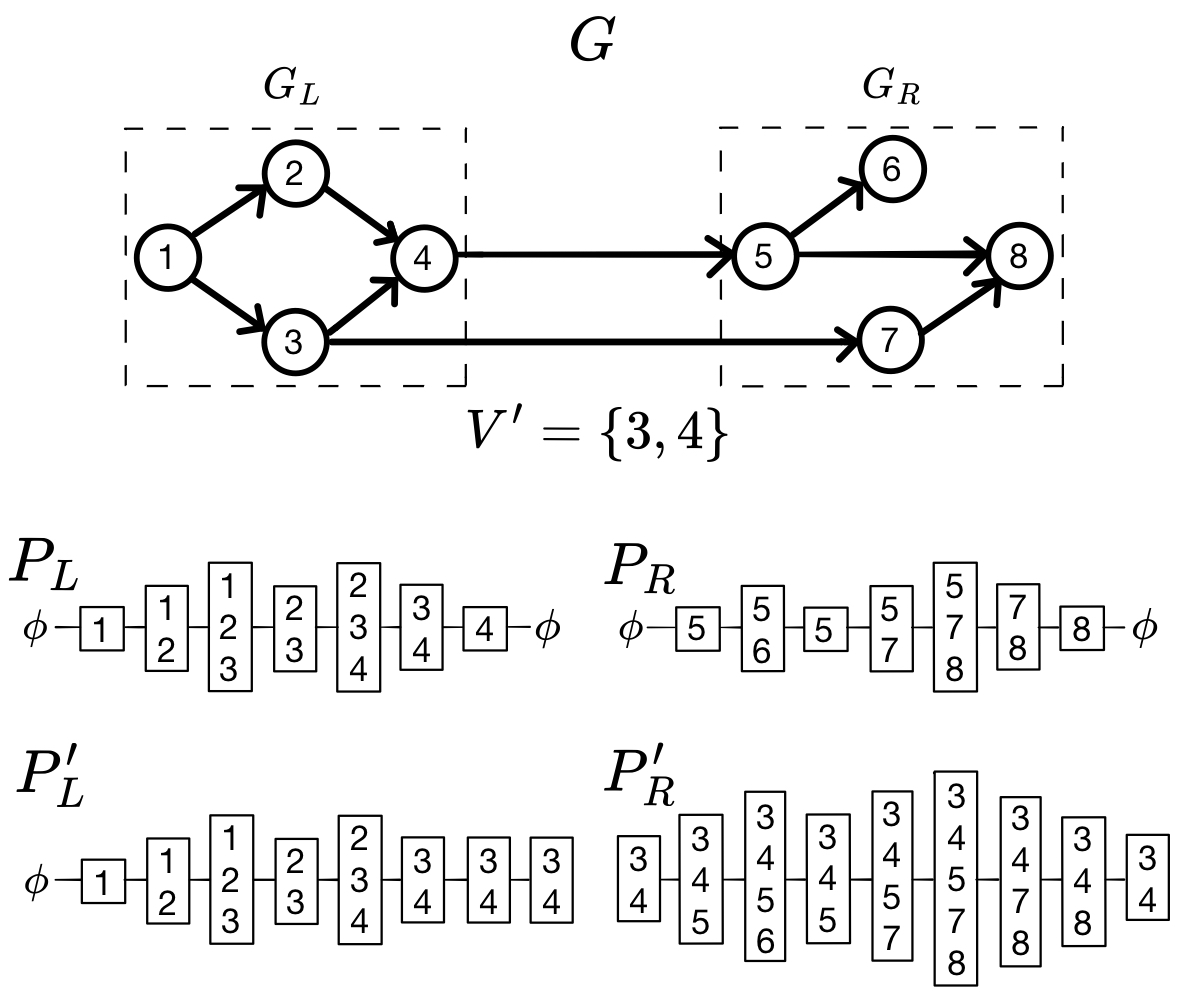
\includegraphics[width=15.0cm]{pic2.jpg}
\caption{$\mathsf{Merge}$の動作の様子.$G_L$の頂点のうち$G_R$に向かう枝を持つ頂点集合$V'$は${3, 4}$となる.受け取った$P_L, P_R$をもとに$V'$の各頂点をバッグに加えた$P'_L, P'_R$を構成し,それらを結合してできるnice DAG-PDを返す.}
\label{fig:2}
\end{figure}
}

次に,DAG $G$が与えられたときに$G$のnice DAG-PDを出力するアルゴリズム$\mathsf{Make}$を示す.

%\vskip\baselineskip

$\mathsf{Make}(G[V])$
\begin{enumerate}
    \item Termination Step: $|V|=1$ならば,$G$の自明なnice DAG-PD $P = (\varnothing, V, \varnothing)$を返す.
    \item Divide Step: $A, B$を,Lemma~\ref{separator_algorithm}のアルゴリズムによる$G$の分割とする.\par
    再帰的に$D_A = \mathsf{Make}(G[A]), D_B = \mathsf{Make}(G[B])$を計算する.
    \item Combine Step: $D = \mathsf{Merge}(G[A], G[B])$とし,$D$を返す.
\end{enumerate}


ここでTheorem~\ref{approximation}の証明のため,次の補題を示す.

\begin{lemma}\label{sepa_pw_relation}
    頂点数$n$,最大出次数$k$,DAG-pathwidth $pw$であるDAG $G$に対し,コストが高々$k(pw+1)$のminimum $\frac{1}{3}$-balanced DAG edge-separatorが存在する.
\end{lemma}

\begin{proof} 
$G=(V, E)$の最適なnice DAG-PDを$P=(X_1, X_2, \dots , X_s)$とする.$P$のDAG-pathwidthは$pw$である.$G$の各頂点を$P$でintroduceされた順に$v_1, v_2, \dots , v_n$とする.$n$が偶数のとき,$v=v_{\frac{n}{2}}$,$n$が奇数のとき,$v=v_{\frac{n+1}{2}}$とし,$v$が初めてintroduceされたバッグを$X_i$とする.$A= X_1 \cup X_2 \cup \dots \cup X_i, B= X_{i+1} \cup X_{i+2} \cup \dots \cup X_s$とする.例としてFiture\ref{fig:3}を示す.このとき$Xi$から出て$B$に入る枝の集合を$S$とすると,DAG-PDのルール3より$G'=(V, E \backslash S)$には$A$と$B$の間に枝はなく,$v$の選び方により$|A| \geq \frac{1}{3}|V|, |B| \geq \frac{1}{3}|V|$を満たす.またDAG-PDのルール2より$A$と$B$の間の枝は$A$から出て$B$に入る向きである.よって$S$は$G$の$\frac{1}{3}$-balanced DAG edge-separatorである.$G$の最大出次数が$k$であることに注意すると,$S$のコスト$C(S)$について以下の不等式が成り立つ.
\begin{align*}
    &C(S) \leq k|X_i| \leq k(pw+1)
\intertext{一方,$G$のminimum $\frac{1}{3}$-balanced DAG edge-separator $S_{opt}$のコストは高々$C(S)$であるから,}
    &C(S_{opt}) \leq k(pw+1)
\end{align*}
\end{proof} 

\ifthenelse{\boolean{Draft}}{
\begin{figure}[t]
\centering
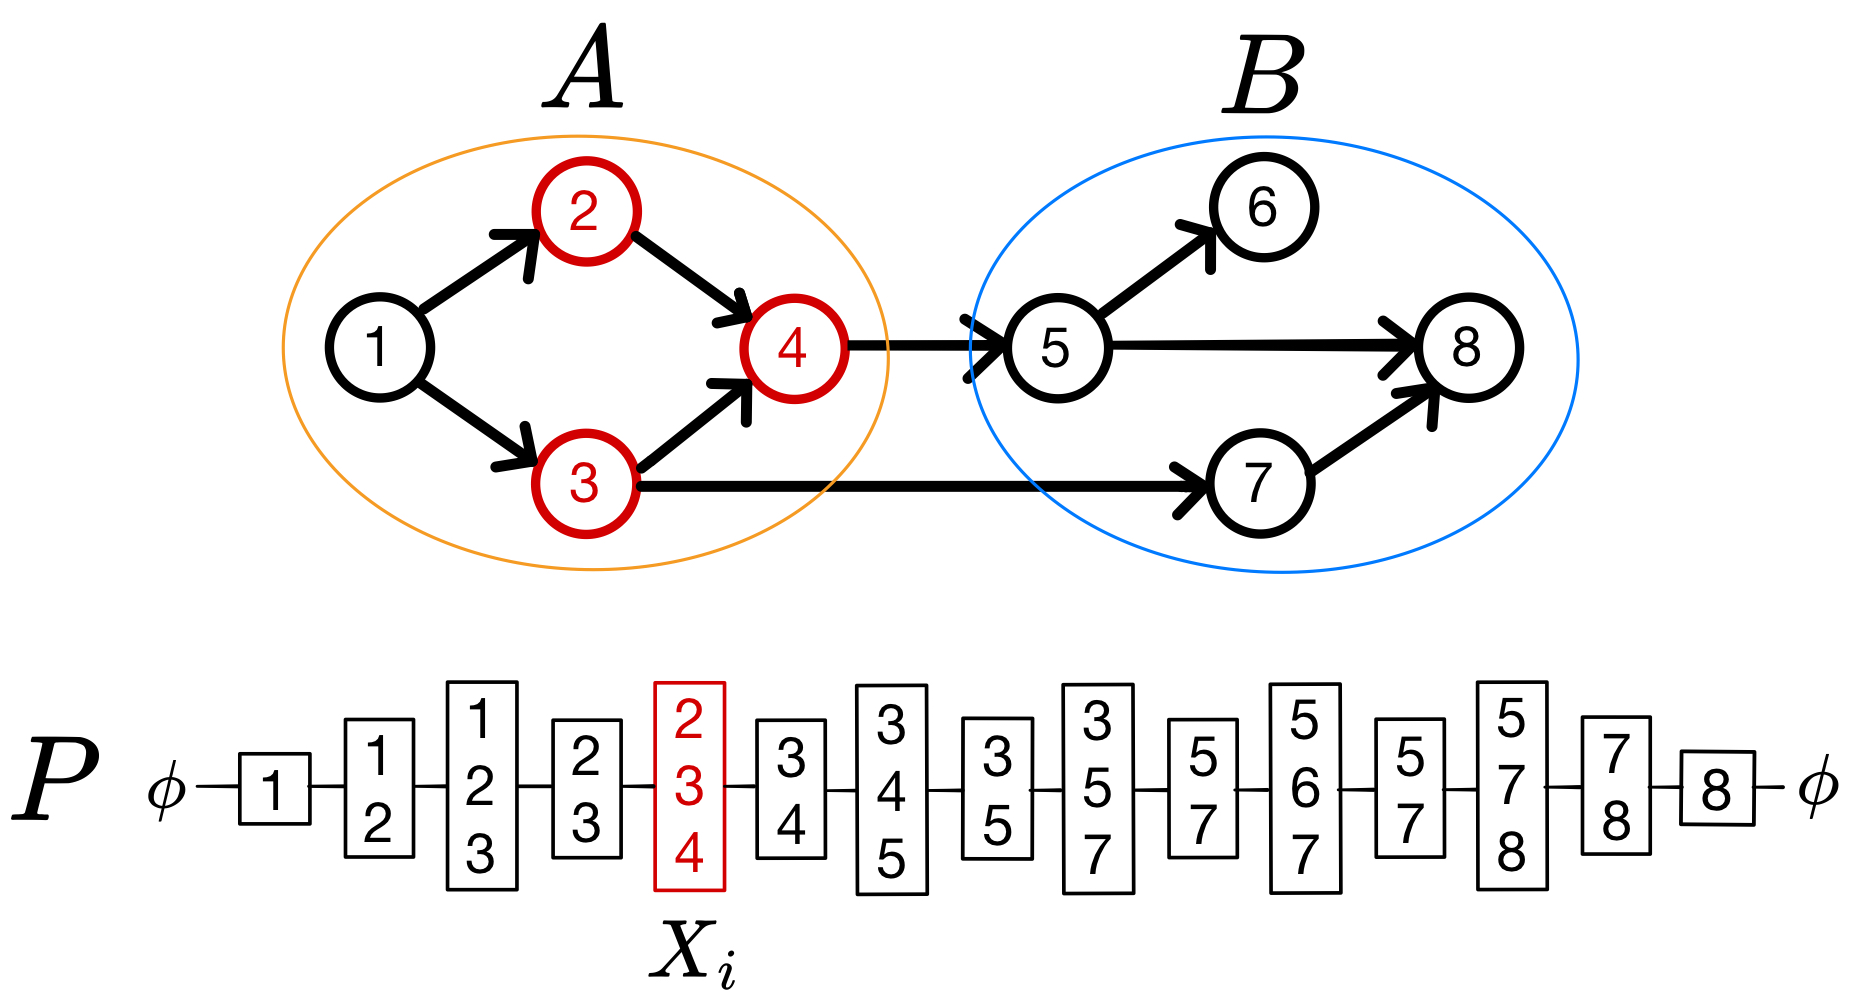
\includegraphics[width=15.0cm]{pic3.jpg}
\caption{最適なnice DAG-PD $P$において,初めて半分以上の頂点がintroduceされたバッグを$X_i$とし,それ以前のバッグの和集合を$A$, 残りの頂点集合を$B$とする.$A, B$のサイズはともに全体の$\frac{1}{3}$以上であり,$A, B$の間の枝は$A$から出て$B$に入る向きである.さらに最大出次数を$k$とすると,$A, B$の間の枝数は高々$k|X_i|$本である.}
\label{fig:3}
\end{figure}
}

最後に次の補題を示すことで,Theorem~\ref{approximation}が成り立つことを示す.

\begin{lemma}
    頂点数$n$,最大出次数$k$,DAG-pathwidthが$pw$のDAG $G[V]$が与えられたとき,$P = \mathsf{Make}(G[V])$とする.このとき,ある定数$\alpha$が存在し,$P$の幅は高々$\alpha k(pw+1)\log ^2 n$である.
\end{lemma}

\begin{proof}
DAG $G_L, G_R$があり,$G_L, G_R$の間の枝は,$G_L$から出て$G_R$に入る向きであるとする.また$G_L, G_R$に対して,あるnice DAG-PD $P_L, P_R$があり,幅がそれぞれ$w_l, w_r$であるとする.ここで$G_L, G_R$の間の枝の端点のうち,$G_L$に含まれる頂点集合を$V'$とする.このとき$\mathsf{Merge}(P_L, P_R)$の動作中に構成される$P'_L, P'_R$の幅は,それぞれ高々$w_l + |V'|, w_r +|V'|$である.なぜならば,$P'_L$は$P_L$の各バッグに高々$|V'|$個の頂点を追加する操作を行い,$P'_R$は$P_R$の各バッグにちょうど$|V'|$個の頂点を追加する操作を行うからである.したがって$\mathsf{Merge}(P_L, P_R)$によって得られるnice DAG-PD $P_{LR}$の幅$w_{lr}$は,
\begin{align*}
    w_{lr}  &\leq \max(w_l + |V'|, w_r + |V'|) \\
            &=  \max(w_l, w_r)+|V'|
    \intertext{$G_L, G_R$の間の枝数を$m$とすると,$|V'|$は高々$m$であるから,}
    w_{lr}  &\leq \max(w_l, w_r) + m
    \intertext{一般性を保って$w_l \leq w_r$とすると,}
    w_{lr}  &\leq  w_r + m
    \intertext{minimum $\frac{1}{3}$-balanced DAG edge-separatorのコストを$m_{opt}$とすると,Lemma~\ref{separator_algorithm}より,ある定数$\alpha$があり,$m \leq \alpha m_{opt}  \log n$とできるため,}
    w_{lr}  &\leq  w_r + \alpha m_{opt}  \log n
    \intertext{$\mathsf{Make}$は$\mathsf{Merge}$を高々$\log n$回繰り返すため,$\mathsf{Make}$が最初に構成するサイズ1のnice DAG-PDの幅が0であることに注意すると,$\mathsf{Make}$が出力するnice DAG-PDの幅$w$は,}
    w       &\leq  0 + (\alpha m_{opt}  \log n)\log n \\
            &= \alpha m_{opt}  \log ^2 n
    \intertext{Lemma~\ref{sepa_pw_relation}より,$m_{opt} \leq k(pw+1)$であるから,}
    w       &\leq \alpha k(pw+1)  \log ^2 n
\end{align*}
以上より,$P$の幅は高々$\alpha k(pw+1)\log ^2 n$である.
\end{proof} 



\subsection{$O(\log ^{3/2} n)$-近似アルゴリズム}

上記のアルゴリズムにより$O(\log ^2 n)$の近似率である幅を持つDAGパス分解を得られるが,以下ではone-shot BPとの等価性を示すことでさらに$O(\log ^{3/2} n)$の近似率が達成できることを示す.

\begin{theorem}\label{approximation2}
    頂点数$n$,DAG-pathwidthが$pw$のDAG $G$が与えられたとき,幅が$O(pw \cdot \log ^{3/2} n)$のDAG-PDを与える多項式時間アルゴリズムが存在する.
\end{theorem}


Perら[20]はone-shot BPの近似アルゴリズムの存在を示している.

\begin{lemma}
    頂点数$n$のDAG $G$に対し,one-shot BPのペブリング数が最小値の高々$O(\log ^{3/2} n)$倍である戦略を出力するアルゴリズムが存在する.
\end{lemma}

したがって,Theorem~\ref{approximation2}を示すためには以下の補題を示せば十分である.

\begin{lemma}\label{lemma_approximation2}
    one-shot BPとnice DAG-PDは等価な問題である.
\end{lemma}

\begin{proof}
    まずDAG $G$に対し,$X$が$G$のnice DAG-PDであれば$X$は$G$のone-shot BPであることを示す.$G$に対するあるnice DAG-PDを$X=(X_1, X_2, \dots, X_s)$とする.ルール4より$X_i = \varnothing$であるためone-shot BPの初期条件を満たす.ルール1とルール3より,すべての頂点は$X$でちょうど1回introduceされるため,one-shot BPですべての頂点がちょうど1回pebbleされるという条件を満たす.操作1とルール2より,$v \in V$が$X_i$でintroduceされるとき,任意の$(u, v)\in E$に対して$u \in X_{i-1}$.これはone-shot BPのpebbleのルールを満たす.また各頂点に対し,forgetがちょうど1度だけ行われることに注意すると,操作2とunpebbleの操作は明らかに等価である.よって$X$のintroduceとforgetが各々pebbleとunpebbleに対応する.以上より$X$は$G$のone-shot BPである.
    
    次に$P$が$G$のone-shot BPであれば$P$は$G$のnice DAG-PDであることを示す.$G$に対するあるone-shot BPを$P=(P_1, P_2, \dots, P_t)$とする.$P_1 = \varnothing$よりnice DAG-PDのルール4を満たす.また各頂点$v \in V$に対し,$v$は$P$でちょうど1回ずつpebble,unpebbleされるため,nice DAG-PDのルール1を満たす.また,$v$のpebble,unpebbleがそれぞれ$P_i, P_{k+1}$ $(1 \leq i \leq k \leq t-1)$で行われるとすると,任意の頂点に対して2回以上pebbleされることはないため,任意の$P_j$ $(i \leq j \leq k)$において$v \in P_j$を満たす.これを$V$の全ての頂点に対して考えることで,nice DAG-PDのルール3を満たす.さらにpebbleのルールより,$v \notin P_{i-1}$かつ任意の$(u, v) \in E$に対し$u \in P_{i-1}$ならば$P_i = P_{i-1} \cup \{v\}$であるが,これは$u, v \in P_i$かつ$v \notin P_{i-1}$を満たす.したがってpebbleの操作はnice DAG-PDのルール2を満たしたintroduceの操作とみなすことができる.またunpebbleの操作は明らかにnice DAG-PDのforgetの条件を満たす.以上より$P$は$G$のnice DAG-PDである.
\end{proof}


















\section{$O(ld^t)$の幅のDAGパス分解を求めるアルゴリズム} %\label{sec_FPTforPathwidth}

本節では最大出次数$d$,根の個数$l$であるDAG $H$と非負整数$t$が与えられたとき,$O(ld^t)$の幅を持つDAG-PDを出力するか,$H$のパス幅が$t$よりも大きいことを示す証拠を与えるFPTアルゴリズムを提案する.

\subsection{無向グラフのパス分解を求めるアルゴリズム}
Kevinら[8]は以下の補題を示している.

\begin{lemma}\label{pathwidth algorithm of undirected graph}
    頂点数$n$の無向グラフ$H$,整数$t$が与えられたとき,$H$のパス幅が$t$より大きい証拠を与えるか,幅が高々$O(2^t)$のパス分解を与えるような$O(n)$の計算時間のアルゴリズムが存在する.
\end{lemma}
\vskip\baselineskip

上記のアルゴリズムを参考にし,最大出次数と根数がそれぞれ$d, l$であるDAG $H$に対し,$H$のパス幅が$t$より大きい証拠を与えるか,幅が高々$O(ld^t)$のパス分解を与えるような多項式時間FPTアルゴリズムを構成する.

\subsection{アルゴリズムの構築}

アルゴリズムでは以下のembeddingを利用する.

\begin{definition*}[embedding]
    有向グラフ$G_1 = (V_1, E_1)$の,有向グラフ$G_2 = (V_2, E_2)$へのembeddingとは,$V_1$から$V_2$への単射であり,かつ任意の枝$(u, v) \in E_1$から$E_2$の有向辺素パスへの写像が存在することである.
\end{definition*}

\vskip\baselineskip
本節では一般のDAGに対して以下が成り立つことを示す.

\begin{theorem}\label{approximation3}
    $H$を最大出次数と根数がそれぞれ$d, l$である任意のDAG,$t$を非負整数とする.このとき以下のいずれか一方が必ず成り立つ.
    \begin{enumerate}
        \item[(a)] $H$のDAGパス幅は高々$ld^{t+3}-1$である.
        \item[(b)] $H$は2つのDAG $A, B$に分割できる.このとき$A$と$B$の間には$A$から$B$への枝しか存在せず,$A$のパス幅は$t$より大きく$ld^{t+3}-1$より小さい.
    \end{enumerate}
\end{theorem}
\vskip\baselineskip




Theorem~\ref{approximation3}を示す前に,以下の補題を示す.

\begin{lemma}\label{comp_tree}
    $T_{h, d}$を高さ$h$の完全有向$d$分木 $(h, d > 1)$とする.このとき$T_{h, d}$のDAGパス幅は$h-1$である.
\end{lemma}

\begin{proof}
    $h$に関する数学的帰納法で示す.$h=2$のとき$T_{2, d}$のパス幅は明らかに1であるため補題を満たす.ここである$h > 1$での補題の成立を仮定する.仮定より幅が$h-1$であるようなDAG-PD $X_h$が存在する.ここで$T_{h+1, d}$は単一の根$r$から$d$個の$T_{h, d}$の根に枝を伸ばしたグラフであることに注意すると,$T_{h+1, d}$の最適なパス分解は,はじめに$r$の根をバッグに含め,以降で$X_h$の各バッグを順に$d$回分つなげたものである.$h, d > 1$に注意すると,このとき明らかに($T_{h+1, d}$のDADパス幅) $= 1 + (h-1) = h$が成り立つため補題を満たす.以上より2以上の任意の$h, d$に対して補題が成り立つ.
\end{proof}



以下では.実際にアルゴリズムを構築することでTheorem~\ref{approximation3}を示す.

\begin{proof}(Theorem~\ref{approximation3})\\
入力グラフ$H = (V, E)$に対し,高さが$\lceil \log_d l \rceil$である完全有向$d$分技(ただし根自身の高さを1とする)を用意し,出次数が高々$d$となるように完全有向$d$分木の葉から$H$の各根に向かう枝を加えて結合する.こうしてできるグラフを$H'$とする.また$M_{t, d, l}$を高さ$\lceil \log_d l \rceil +t+2$の完全有向$d$分木とする.

以下のアルゴリズムでは$M_{t, d, l}$の$H'$へのembeddingを見つける.もしembeddingを見つけることができれば$H'$のDAGパス幅は$M_{t, d, l}$のDAGパス幅以上であることがわかる.embeddingの探索では部分的なembeddingを行い,$M_{t, d, l}$の頂点をトークンと呼ぶ.token $T$が$H'$のある頂点に置かれたとき$T$はtokenedであると表し,頂点に置かれていないときuntokenedであると表す.アルゴリズムを通して$H'$の1つの頂点に置くことができるトークンは1つのみである.

以下で各トークンの再帰的なラベル付けを与える.図\ref{fig:10}で$H$に対する$H', M_{t, d, l}$の構成例を示す.

\begin{enumerate}
    \item 根のトークンは空文字列$\lambda$とラベル付けする.
    \item 高さ$h$の親トークン$m=\lambda b_1 b_2 \dots b_{h-1}$の子トークンを左から順に$m \cdot 1, m \cdot 2, \dots , m \cdot d$とラベル付けする.
\end{enumerate}

時刻$i$においてトークンが置かれた$H'$の頂点集合を$X_i$とする.頂点集合の列$(X_1, X_2, \dots, X_s)$は$H'$のパス分解,もしくは$H'$の分割でTheorem~\ref{approximation3}の条件を満たす$A'$のパス分解を表す.


アルゴリズムの初期状態では$H'$のすべての頂点がblueで塗られていると仮定する.アルゴリズムの進行中,$H'$のある頂点$v$にトークンが置かれた場合,$v$の色をredに変更し,トークンが$v$から削除されてもredのままであるとする.このときblueの頂点にのみトークンを置くことができるため,$H'$の各頂点は高々一度しかトークンを置くことができない.


\ifthenelse{\boolean{Draft}}{
\begin{figure}[t]
    \centering
    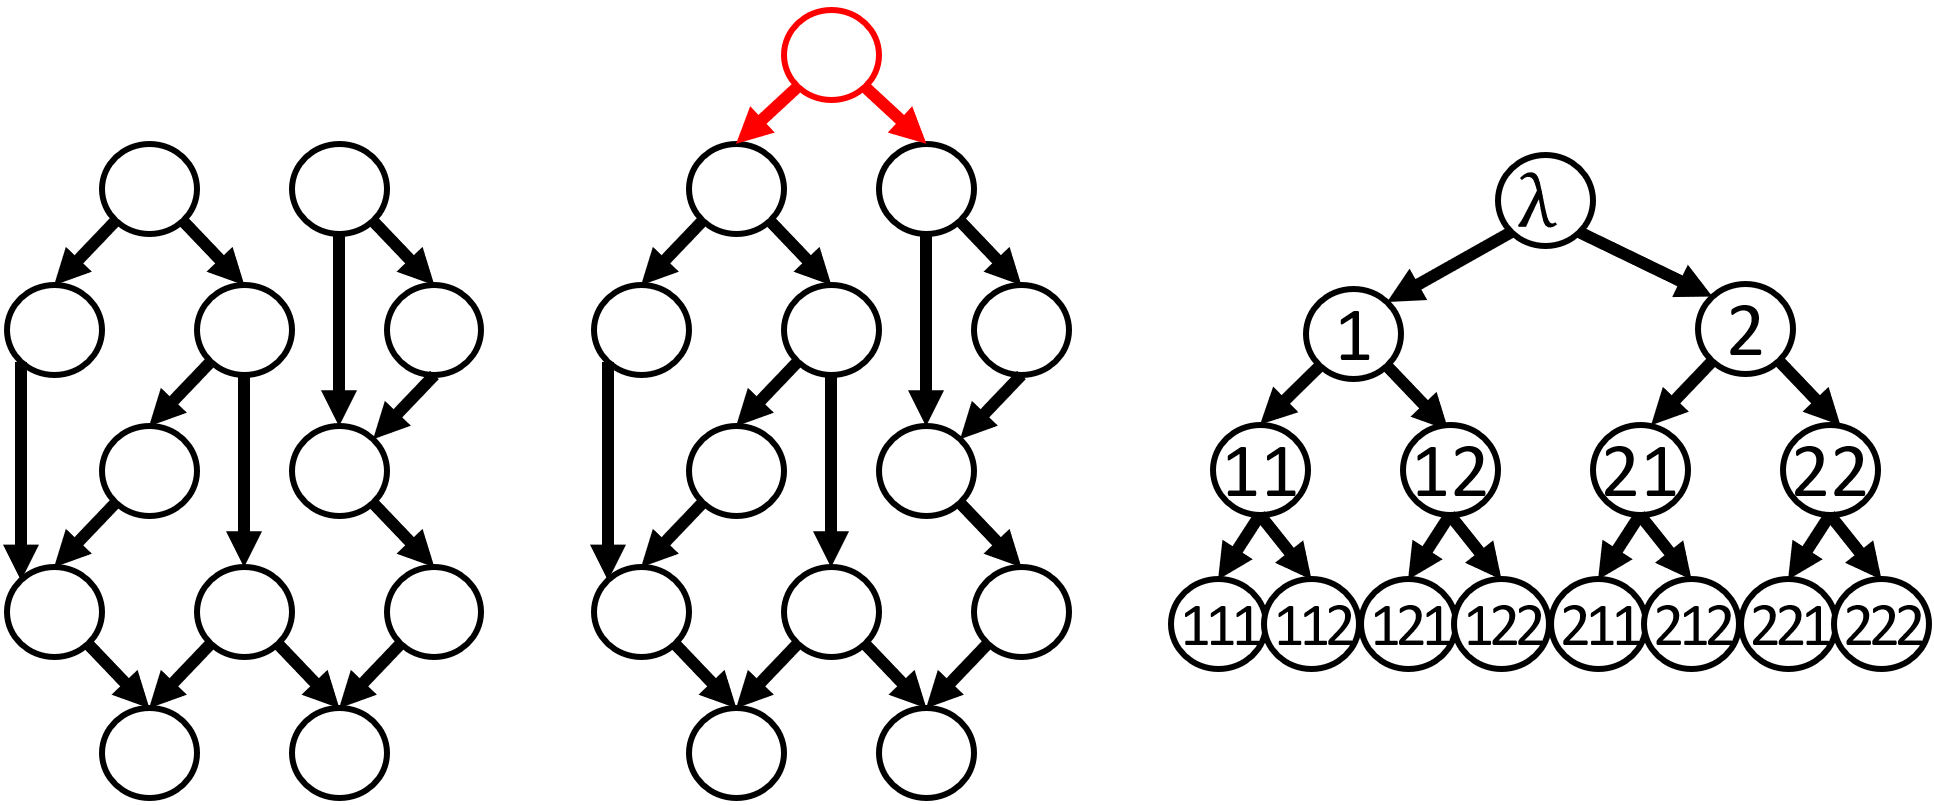
\includegraphics[width=15.0cm]{pic10.png}
    \caption{$d=2, l=2$である$H$(左)と$t=1$が与えられたときの$H'$(中央)と$M_{t, d, l}$(左)の構成.$H$の各根につながる完全有向$d$分木(赤部分)を追加したものが$H'$である.また$M_{t, d, l}$のラベル付けでは親のラベルに対して文字を1つ右につなげることで再帰的に構成する.}
    \label{fig:10}
\end{figure}
}




\begin{figure}[!t]
\begin{algorithm}[H]
	\caption{$\mathsf{GrowTokenTree}$}
	\label{growtokentree}
	\begin{algorithmic}[1]
    \WHILE{there is a vertex $u \in H'$ with token $T$ and a blue neighbor $v$ whose all predecessors are placed token, and token $T$ has an untokened child $T \cdot b$}
    \STATE place token $T \cdot b$ on $v$
    \ENDWHILE
    \RETURN \{tokened vertices of $H'$\}
	\end{algorithmic}
\end{algorithm}
\end{figure}



\begin{figure}[!t]
\begin{algorithm}[H]
    \caption{$\mathsf{FindEmbedding}$}
	\label{findEmbedding}
	\begin{algorithmic}[1]
    \STATE place root token $\lambda$ on root of $H'$
    \STATE $i \leftarrow 1$
    \STATE $X_i  \leftarrow$ call $\mathsf{GrowTokenTree}$
    \WHILE{$|X_i| < |V[M_{t, d, l}]|$ and $H'$ has at least one blue vertex}
    \IF{there is a vertex $v \in H'$ with token $T$ that $v$ has no blue successor and $T$ has at most one tokened child}
    %\STATE let $\mathcal{T} = \{T\}$ that each $T$ satisfies above conditions. Among $T \in \mathcal{T}$, let $T'$ be the one included in the highest layer of $M_{t, d, l}$
    \STATE remove $T$ from $H'$
    \IF{$T$ had one tokened child $T \cdot b$}
    \STATE replece $T \cdot b$ with $T$ on $H'$
    \ENDIF
    \WHILE{$T$ had a tokened grandchild $T \cdot b_1 \cdot b_2$, and $T \cdot b_2$ is untokened}
    \STATE replece $T \cdot b_1 \cdot b_2$ with $T \cdot b_2$ on $H'$
    \ENDWHILE
    \ELSE
    \RETURN $X_i$
    \ENDIF
    \STATE $i \leftarrow i+1$
    \STATE $X_i \leftarrow$ call $\mathsf{GrowTokenTree}$
    \ENDWHILE
	\end{algorithmic}
\end{algorithm}
\end{figure}


アルゴリズム$\mathsf{FindEmbedding}$は,(1)列4で$H'$がblueの頂点を持たなくなったときか,(2)列4で$|X_i| = |V[M_{t, d, l}]|$が成り立つときか,(3)列14の処理が行われたときのいずれかで終了する.以下では(1)(2)(3)のそれぞれの場合においてアルゴリズムが正しく動作することを示す.

まず(1)の場合を考える.$\mathsf{FindEmbedding}$の列4において$i=s$の時点で$H'$のすべての頂点がredになって終了した場合,アルゴリズムが出力する頂点集合の列$X_{H'} = (X_1, X_2, \dots , X_s)$は$H'$のDAG-PDになっていることを示す.まず任意の頂点$v \in H'$はredであるためいずれかの頂点集合$X_i$に必ず含まれる.よってDAG-PDのルール1を満たす.また$v$はちょうど1度だけblueからredに変わり,redのときにのみトークンが削除されてそれ以降tokenが置かれることはないため,$v$を含む頂点集合$X_i$は連結なパスを構成する.したがってDAG-PDのルール3を満たす.さらに任意の枝$(u, v) \in E[H']$について$v$がblueからredに変わる時点を$i$とする.このとき$\mathsf{FindEmbedding}$の列5の条件より$i$より前の時点で$u$からtokenは削除されず,また$\mathsf{GrowTokenTree}$のwhileの条件より,$v$の先行頂点にはすべてtokenが置かれているため,$u$もまた$X_i$に含まれる.$v$は$X_{i'}$ $(i' < i)$に含まれないことに注意すると$u, v \in X_i, v \notin X_{i-1}$が成り立つためDAG-PDのルール3を満たす.以上より頂点集合の列$X_{H'}$は$H'$のDAG-PDとなっている.$\lceil \log_d l \rceil < \log_d l +1$に注意すると,このとき$X_{H'}$の幅は高々$|V[M_{t, d, l}]| = d^{\lceil \log_d l \rceil +t+2}-1 < ld^{t+3}-1$である.ここで$X_H = (X_1 \cap V[H], X_2 \cap V[H], \dots , X_s \cap V[H])$は$H$に対してDAG-PDの3つのルールを満たすことから$H$のDAG-PDになっていることに注意すると,$X_H$の幅もまた高々$ld^{t+3}-1$である.したがって幅が高々$ld^{t+3}-1$である$H$のDAG-PDが得られる.

次に(2)の場合を考える.$\mathsf{FindEmbedding}$の列4において$i=s$の時点で$|X_s| = |V[M_{t, d, l}]|$が成り立つとき,頂点集合$X_1 \cup X_2 \cup \dots \cup X_s$によって誘導される$H'$の部分グラフを$A'$とする.このときアルゴリズムが出力する頂点集合の列$X_{A'} = (X_1, X_2, \dots , X_s)$は$A'$のDAG-PDになっている.まず$A'$の定義より明らかにDAG-PDのルール1を満たす.また上記と同様の議論によりDAG-PDのルール2, 3を満たす.よって$X_{A'}$は$A'$のDAG-PDである.ここで$A$を頂点集合$V[A'] \cap V[H]$によって誘導される部分グラフとし,$X_A = (X_1 \cap V[H], X_2 \cap V[H], \dots , X_s \cap V[H])$とする.$X_A$は$A$に対してDAG-PDの3つのルールを満たすことから$A$のDAG-PDになっていることに注意すると,上記と同様の議論により幅が高々$ld^{t+3}-1$である$A$のDAG-PDが得られる.

さらに,$X_{A'}$の右端のバッグ$X_s$によって誘導される$H'$の部分グラフ$H_{A'3}$は,$M_{t, d, l}$の$H'$へのembeddingを表していることを示す.$\mathsf{GrowTokenTree}$では$u, v \in H'$にそれぞれトークン$T, T\cdot b \in M_{t, d, l}$を配置する操作なので,明らかにembeddingの条件を満たす.したがって$\mathsf{FindEmbedding}$の列6から列12においてembeddingの条件が満たされることを示せば十分である.列5の処理の時点で$M_{t, d, l}$の各頂点に対してembeddingの条件が満たされていると仮定する.列5の条件を満たすトークン$T$が存在し,tokenedな子を1つだけ持つとき,列6と列8により$T \cdot b$は$T$に置き換えられる.このとき$T$の親$T'$と$T, T \cdot b$のそれぞれ置かれていた頂点を$u, v, w \in H'$とすると,置き換えによって$w$に$T$が置かれるが,仮定より枝$(T', T)$から辺素パス$u \rightarrow v$への写像があるため,$T$はただ一つのtokenedな子$T \cdot b$をもつことに注意して,明らかに枝$(T', T)$から辺素パス$u \rightarrow w$への写像が存在する.したがってembeddingの条件は満たされる.$T$がtokenedな子を持たないときは列6のみ実行され,列8は実行されないが,$T$を削除しても明らかにembeddingの条件は満たされる.次に列10から12の処理を考える.$\mathsf{GrowTokenTree}$では$M_{t, d, l}$の根に近いトークンから順にtokenedになるため,$T$がtokenedな子を持たないならば$T$の孫もまたtokenedでない.したがって列11は行われない.$T$がただ一つのtokenedな子$T \cdot b_1$を持つ場合,$\mathsf{GrowTokenTree}$の操作と$T$がtokenedな子を持たない場合の操作より,$T$のtokenedな孫は必ず$T \cdot b_1$を親に持つ.ここで列8の処理により$T \cdot b_1$がuntokenedになるため$T$のすべての子がuntokenedとなるが,列11の処理によりtokenedな$T$の孫$T \cdot b_1 \cdot b_2$はすべて$T$の子$T \cdot b_2$に置き換えられる.このとき$T \cdot b_1, T \cdot b_1 \cdot b_2$が置かれていた頂点をそれぞれ$u, v \in H'$とすると,仮定より$M_{t, d, l}$の枝$(T \cdot b_1, T \cdot b_1 \cdot b_2)$から$H'$の辺素パス$u \rightarrow v$への写像があるため,トークンの置き換え後は明らかに枝$(T, T \cdot b_2)$から辺素パス$u \rightarrow v$への写像が存在する.したがってembeddingの条件は満たされる.

以上より$X_{A'}$が出力されるとき,$A'$は$M_{t, d, l}$の$H'$へのembeddingを表している.ここで$A'$は高さ$\lceil \log_d l \rceil +t+2$の完全有向$d$分木を含み,頂点集合$V[A'] \backslash V[A]$によって誘導される部分グラフは高さが高々$\lceil \log_d l \rceil$の完全有向$d$分木であることに注意すると,$A$は少なくとも$(\lceil \log_d l \rceil +t+2) -(\lceil \log_d l \rceil) = t+2$の高さをもつ完全有向$d$分木$T_A$を含む.すなわち$T_A$から$A$へのembeddingが存在する.Lemma~\ref{comp_tree}より$T_A$のパス幅は$t+1$であるため,$A$のパス幅もまた$t+1$以上である.よって$A$を内部に含む$H$のパス幅は$t$より大きいことが示される.

最後に(3)の場合を考える.$\mathsf{FindEmbedding}$の列14の処理が行われたときに$A$のパス幅が$t$より大きいことを示す.ここで単一の根$r_G$をもつ任意のDAG $G$の各頂点に対し,$r_G$からの最長パスの長さが$k-1$である頂点集合を$L_{G, k}$と表す.以下では$k$を$G$の階層と呼ぶ.ただし$L_{G, 1} = \{r_G\}$とする.$H'$の各頂点の出次数は高々$d$であるため,ある時点$i$において$\lambda \in M_{t, d, l}$が置かれた頂点$r'$の階層を$k_{r'}$,頂点集合$\bigcup_{k_{r'} \leq k \leq k_{r'}+ \lceil \log_d l \rceil +t+1} L_{H', k}$によって誘導される部分グラフを$H_{k_{r'}, t}$とすると,$H_{k_{r'}, t}$に含まれる任意の頂点にはトークンを置くことができる.ここで列14の処理が行われるとき,任意の頂点$v \in V[H_{k_{r'}, t}]$は以下の少なくとも一方が成り立つ.

\begin{enumerate}
    \item ある$w \in \mathsf{suc}(v)$が存在し,$w \in L_{H, k'}$ $(k' > k_{r'}+ \lceil \log_d l \rceil +t+1)$を満たし,かつ$w$はblueである. \label{cond1}
    \item $v$に置かれたトークン$T$が2つ以上のtokenedな子をもつ. \label{cond2}
\end{enumerate}

また,このとき$M_{t, d, l}$においてtokenedであるトークンのパス$\lambda \cdot m_1 \cdot m_2 \cdot \dots m_{\lceil \log_d l \rceil +t+1}$が少なくとも1つ存在する.なぜならば,もしそのようなパスが存在しなければ,上記の議論により$H_{k_{r'}, t}$は階層が高々$\lceil \log_d l \rceil +t+1$しかなく,$H_{k_{r'}, t}$のすべての頂点にトークンを置くことができ矛盾するからである.ここで$P = \lambda \cdot m_1 \cdot m_2 \cdot \dots m_{\lceil \log_d l \rceil +t+1}$とすると,各トークン$m_i \in P$ (ただし$\lambda$を$m_0$と表現する)について$m_i$が置かれた頂点$v_i$は上記の条件\ref{cond1}, \ref{cond2}の少なくとも一方を満たす.条件\ref{cond1}を満たすとき,$v_i$は$v_{\lceil \log_d l \rceil +t+1}$にトークン$m_{\lceil \log_d l \rceil +t+1}$が置かれるまでは$A$のDAG-PDにおいてforgetすることはできない.なぜならばDAG-PDのルール2より,条件\ref{cond1}での$w$のintroduceは$v_{\lceil \log_d l \rceil +t+1}$のintroduceの後,すなわちトークン$m_{\lceil \log_d l \rceil +t+1}$の$v_{\lceil \log_d l \rceil +t+1}$への配置後であり,$w$を後続頂点にもつ$v_i$はそれよりも前にforgetできないからである.このとき$u_i=v_i$とする.$m_i$が条件\ref{cond1}を満たさず\ref{cond2}を満たすとき,$m_i$はtokenedな子$m'_{i+1}\ (\neq m_{i+1})$を少なくとも1つもつ.$m'_{i+1}$が置かれた頂点についても条件\ref{cond1},\ref{cond2}の少なくとも一方を満たすため,上記の議論を繰り返すことにより,$M_{t, d, l}$のtokenedな葉は条件\ref{cond1}を満たすことに注意すると,$m'_{i+1}$を根とする有向木には条件\ref{cond1}を満たすような頂点が少なくとも1つ存在する.このような頂点を$u_i$とする.上記と同様の理由により,$u_i$は$v_{\lceil \log_d l \rceil +t+1}$に$m_{\lceil \log_d l \rceil +t+1}$が置かれるまでは$A'$のDAG-PDにおいてforgetすることができない.これをすべての$m_i \in P$に対して考えることにより,各頂点$u_0, u_1, \dots, u_{\lceil \log_d l \rceil +t+1}$を得る.このとき$A'$の任意のDAGパス分解$X'$において$v_{\lceil \log_d l \rceil +t+1}$のintroduceを行うバッグを$X_p$とすると,DAGパス分解のルール2に注意して$X'$のバッグ$X_1$から$X_p$までの間では少なくとも各$v_i$ $(0 \leq i \leq \lceil \log_d l \rceil +t+1)$のintroduceが行われており,かつ先程の議論により$X_p$には各$i$に対して$v_i$から$u_i$までのパス上の頂点が少なくとも1つずつ含まれることがいえる.したがって$|X_p| \geq |P| = \lceil \log_d l \rceil +t+2$より,$A'$のパス幅は少なくとも$\lceil \log_d l \rceil +t+1$以上である.ここでトークン列$P$のうち$A$の頂点に置かれたトークンのみを取り出してできるトークン列を$P_A$とする.$|P \backslash P_A| \leq \lceil \log_d l \rceil$より$|P_A| = |P| - |P \backslash P_A| \geq (\lceil \log_d l \rceil +t+2) - \lceil \log_d l \rceil = t+2$に注意すると,上記と同様の議論により$A$のパス幅は$t$より大きいことが示される.
\end{proof}




\begin{cor}
    最大出次数$d$,根の個数$l$であるDAG $H$,整数$t$が与えられたとき,$H$のDAGパス幅が$t$より大きい証拠を与えるか,幅が高々$O(ld^t)$のDAGパス分解を与えるような$O(n^2)$時間のアルゴリズムが存在する.
\end{cor}

\begin{proof}
    Theorem~\ref{approximation3}より,$\mathsf{FindEmbedding}$は$H$のDAGパス幅が$t$より大きい証拠として完全$d$分木の$H$へのembeddingを出力するか,幅が高々$O(ld^t)$のパス分解を出力する.以下では$\mathsf{FindEmbedding}$が多項式時間で終了することを示す.$\mathsf{GrowTokenTree}$では列1のwhileの条件の判定は高々$O(dn)$かかり,これを高々$|V[M_{t, d, l}]| = O(d^t)$回繰り返す.また$\mathsf{FindEmbedding}$の列6の$T$の削除によって,$T$が置かれていた頂点はredのままであるため,この操作は高々$O(n)$回行われることに注意すると,列4のwhileもまた高々$O(n)$回行われる.さらに列10のwhileは明らかに高々$d^2$回繰り返す.他のステップは$O(1)$の計算時間で処理される.以上よりアルゴリズムは$d, l$がある定数以下であるとすると$O(n^2)$で停止する.
\end{proof}



















\section{DAG-treewidth} %\label{sec_DAGtreewidth}

\subsection{DAG-treewidthの定義}

本節では,DAG-PDをさらに一般化した概念であるDAG Tree Decomposition(DAG-TD)を導入する.

\begin{definition*}
 有向グラフ$G=(V, E)$のDAG Tree Decomposition (DAG-TD)とは,有向木$T$と,$T$の各ノード$t$について$\beta(t) \subseteq V$であるような$\beta$とのペア$(T, \beta)$である.$(T, \beta)$は以下の3つを満たす.
 
\begin{enumerate}
    \item $\sum_{t\in T} \beta(t) = V$ 
    \item $T$の根を$r$としたとき,任意の枝 $ (u, v) \in E $ について以下のいずれかが成り立つ.
    \begin{itemize}
          \item $u, v \in \beta(r)$
          \item ある $i$ $(i \in T, i \neq r)$があり,$i$の親を$j$としたとき,$u, v \in \beta(i)$, $v \notin \beta(j)$
    \end{itemize}
    \item 任意の$ i, j, k \in T$に対し,$j$が$i$から$k$までのパス上に存在するならば,$\beta(i) \cap \beta(k) \subseteq \beta(j)$.すなわち各$v \in V$について,$v$を含むバッグは$T$上で非空な部分有向木を誘導する.
    \end{enumerate}
\end{definition*}


\ifthenelse{\boolean{Draft}}{
\begin{figure}[t]
    \centering
    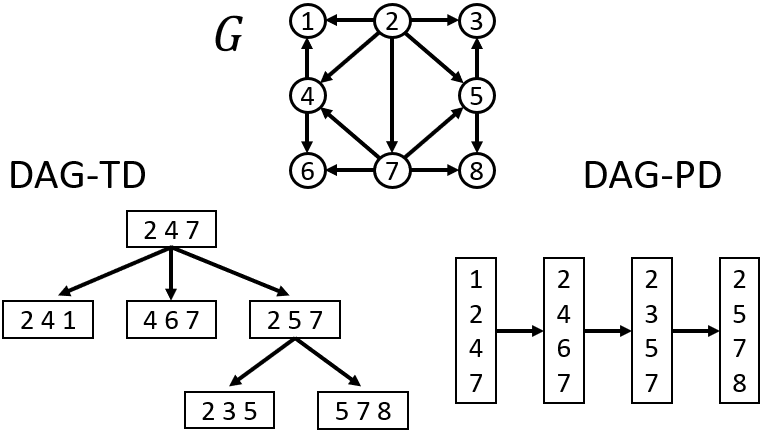
\includegraphics[width=15.0cm]{pic6.png}
    \caption{$G$に対するDAG-TDとDAG-PDの構成例.DAG-TD上での1つのパスは,$G$のある部分グラフに対するDAG-PDになっている.またDAG-PDもDAG-TDの一つであり,DAG-treewidthはDAG-Pathwidthより大きくならない.}
    \label{fig:6}
\end{figure}
}

DAG-TDの例をFigure\ref{fig:6}で示す.以下でDAG-treewidthを定義する.

\begin{definition*}[DAG-treewidth]
    あるDAG-TD $(T, \beta)$のwidthを$\max_{t \in T}|\beta(t)|$と定義する.このとき,有向グラフ$G$のDAG-treewidthとは,$G$に対する全てのDAG-TDのうち,widthが最小であるDAG-TDのwidthである.
\end{definition*}

以降では,$G$のDAG-pathwidth, DAG-treewidthをそれぞれ$\mathsf{pw}(G), \mathsf{tw}(G)$と表す.


\subsection{nice DAG-TD}

本節では,nice DAG-PDと類似の概念であるnice DAG-TDを説明する.

\begin{definition*}
 $G=(V, E)$を有向グラフとし,$(T, \beta)$を$G$のDAG-TDとする.$(T, \beta)$が以下の2つを満たすとき,$(T, \beta)$は$G$のnice DAG-TDであるという.
 
\begin{enumerate}
    \item $r$を$T$の根としたとき,$\beta(r) = \varnothing$ 
    \item 各$i \in T$に対し,$\beta(i)$は以下のいずれかである.
    \begin{description}
          \item[introduce] $i$がただ1つの子$j$をもち,ある強連結成分$S$があり,$S \cap \beta(j) \neq \varnothing$かつ$\beta(i) = \beta(j) \cup S$
          \item[forget] $i$がただ1つの子$j$をもち,ある$v \in V$があり,$\beta(i) = \beta(j) \backslash \{v\}$
          \item[union] $i$がちょうど2つの子$j, k$をもち,$\beta(i) = \beta(j) = \beta(k)$
    \end{description}
    \end{enumerate}
\end{definition*}

\ifthenelse{\boolean{Draft}}{
\begin{figure}[t]
    \centering
    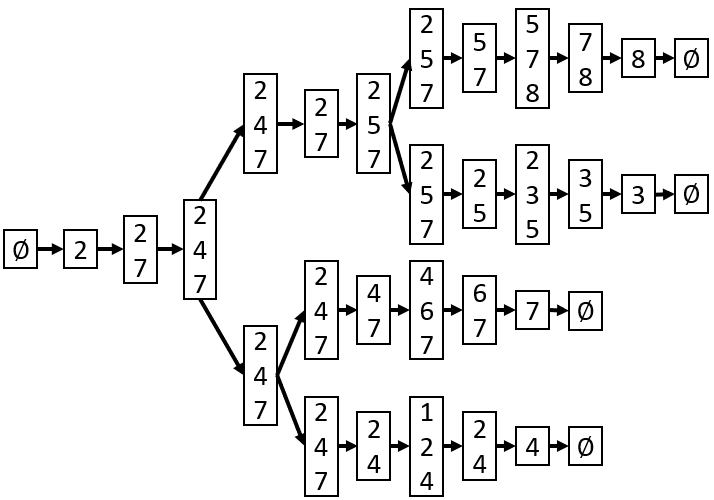
\includegraphics[width=15.0cm]{pic7.png}
    \caption{Figure\ref{fig:6}の$G$に対するnice DAG-TDの構成例.1つの根と複数のsinkをもち,それぞれ空集合からなる.それ以外のバッグは,親のバッグに対して強連結成分が1つ加えられたintroduceか,頂点が1つ除かれたforget,もしくは自身と同じ兄弟をもつunionのいずれかとなる.任意のDAG-TDから,同じwidthをもったnice DAG-TDを効率よく構築できる.}
    \label{fig:7}
\end{figure}
}

nice DAG-TDの例をFigure\ref{fig:7}で示す.あるDAG-TDが与えられたとき,widthが同じである$G$のnice DAG-TDを効率よく構築することができる.

\begin{theorem}
    $(T, \beta)$が有向グラフ$G=(V, E)$のDAG-TDであるとする.また$(T, \beta)$のwidthを$w$とする.このとき,widthが$w$であるような$G$のnice DAG-TDを多項式時間で構築できる.
\end{theorem}

\begin{proof}
    $(T, \beta)$に対し,以下の手順を行いnice DAG-PDを得る.

    \begin{enumerate}
        \item $T$に根$r$ $(\beta(r) = \varnothing)$を追加する.
        \item ある$i \in T$がただ1つの子$j \in T$をもち,かつ$\beta(i) = \beta(j)$ならば,$T$から$j$を除き,$i$から$j$のそれぞれの子への枝を加える.このような$i, j$がなくなるまでこの操作を繰り返す.
        \item 以下の5つの状態がなくなるまで操作を繰り返す.
        \begin{enumerate}
            \item ある$i \in T$と,その子$j \in T$について,$\beta(i) \nsubseteq \beta(j)$かつ$\beta(j) \nsubseteq \beta(i)$ならば,$i$と$j$の間に$i'$ $(\beta(i') = \beta(i) \cap \beta(j))$を加え,$(i, i', j)$の順につなぐ.
            \item ある$i \in T$と,その子$j \in T$について,$\beta(j) \subseteq \beta(i)$かつ$|\beta(i)| - |\beta(j)| \geq 2$ならば,$i$と$j$の間に$i''$ $(\beta(i'') = \beta(i) \backslash \{v\}, v \in \beta(i) \backslash \beta(j))$を加え,$(i, i'', j)$の順につなぐ.
            \item ある$i \in T$と,その子$j \in T$について,$\beta(i) \subseteq \beta(j)$かつ$\beta(j) \backslash \beta(i)$が強連結成分でないとき,$i$と$j$の間に$i'''$ $(\beta(i''') = \beta(j) \backslash A$,$A$は$\beta(j) \backslash \beta(i)$の強連結成分)を加え,$(i, i''', j)$の順につなぐ.
            \item ある$i$が$k$ $(k \geq 3)$個以上の子を持つとき,$i$の直後に,高さが$\lfloor \log_{2} k \rfloor$の完全二分有向木$T'$ $(^{\forall}t' \in T'$について$\beta(t') = \beta(i))$を追加し,$T'$の各葉に対して2つずつ$i$の子を接続し,枝の向きは葉から子への向きとする.ただし,$\lfloor x \rfloor$は$x$を超えない最大の整数値とする.
            \item ある$i$が2つの子$j, k$を持つとき,$i$と$j$,$i$と$k$の間にそれぞれ$j', k'$ $(\beta(j') = \beta(k') = \beta(i))$を追加し,それぞれ$(i, j', j),\ (i, k', k)$の順につなぐ.
        \end{enumerate}
    \end{enumerate}

    以上の操作によってできるDAG-TDは,widthが高々$w$であり,また$G$のnice DAG-TDである.この構築は$G$の頂点数の多項式時間で行える.
\end{proof}


\subsection{計算量クラス}

\begin{theorem}\label{NP困難}
    有向グラフ$G$が与えられたとき,$G$のDAG-treewidthを計算する問題はNP困難である.
\end{theorem}

Theorem~\ref{NP困難}の証明は付録で示す.

\begin{comment}

Theorem~\ref{NP困難}を証明するために,まず以下のLemmaを示す.

\begin{lemma}\label{sink}
    有向グラフ$G=(V, E)$の強連結成分$A$があり,$A$から$V \backslash A$への枝が存在しないとき,$A$を$G$の$sink$と呼ぶ.このとき,$G$が$sink$をただ1つしか持たないならば,$\mathsf{tw}(G) = \mathsf{pw}(G)$が成り立つ.
\end{lemma}


\begin{proof}
    DAG-PD, DAG-TDの定義より,widthが$\mathsf{pw}(G)$である$G$のDAG-PDは$G$のDAG-TDでもある.よって$\mathsf{tw}(G) \leq \mathsf{pw}(G)$が成り立つ.一方,widthが$\mathsf{tw}(G)$である$G$のnice DAG-TDを$(T, \gamma)$とし,sink$A$を含む$T$のバッグのうち,根$r \in T$からの距離が最も近いものを$\gamma(t_i)$ $(t_i \in T)$とする.$T$上で$r$から$t_i$までのパスを$P \subseteq T$としたとき,$(P, \gamma)$が$G$のDAG-PDとなっていることを示す.まず,$P$について$\sum_{p \in P} \gamma(p) = V$が成り立つ.なぜならば,$T$上で$P$に含まれない$P'$があり,かつ任意の$p \in P$に対し,$P'$上で,ある$v \notin \gamma(p)$がintroduceされたとすると,頂点集合$\sum_{p' \in P'} \gamma(p')$が誘導する$G$の部分有向グラフはあるsink$A'$をもつが,$p_A \in P$ $(A \subseteq \gamma(p_A))$と$p_{A'} \in P'$ $(A \subseteq \gamma(p_{A'}))$は非連結であるから,DAG-TDの定義より,$A \neq A'$である.これは$G$がsinkをただ1つしかもたないことと矛盾する.したがって$\sum_{p \in P} \gamma(p) = V$が成り立つことがいえ,$(P, \gamma)$はDAG-PDのルール1を満たす.またDAG-TDのルール2と,$P$がパスであることから$(P, \gamma)$はDAG-PDのルール2を満たす.さらに$P$はパスであるからルール3も満たす.よって$(P, \gamma)$は$G$のDAG-PDである.したがって$\mathsf{pw}(G) \leq \mathsf{tw}(G)$がいえる.以上より,$\mathsf{tw}(G) = \mathsf{pw}(G)$が示される.
\end{proof}


上のLemmaを用い,[3]の手法を参考にしてTheorem~\ref{NP困難}を示す.

\begin{proof}[proof of Theorem~\ref{NP困難}]
    ある有向グラフ$G = (V, E)$が与えられたとき,以下の手順で有向グラフ$G' = (V', E')$ $(|V'| = 2|V| + 1, |E'| = \frac{1}{2}(|V|^2 + 3|V|) + 2|E|)$を構成する.

    \vskip\baselineskip
    \begin{itemize}
        \item $V = \{v_i | i = 1, 2, \dots, n\}$としたとき,$V' = \{v_i, v'_{i} | i = 1, 2, \dots, n\} \cup \{s\}$とする.
        \item $(v_i, v_j)$ $(v_i, v_u \in V', 1 \leq i < j \leq n)$の全ての組合せに対し,$(v_i, v_j) \in E'$とする.
        \item 各$i$ $(i = 1, 2, \dots, n)$に対し,$(v_i, v'_i),\ (v'_i, s) \in E'$とする.
        \item $v_p, v_q \in V$ について$(v_p, v_q) \in E$であるならば,$(v_p, v'_q),\ (v_q, v'_p),\ (v'_p, v'_q) \in E'$とする.
    \end{itemize}
    
    以上の操作によってできる有向グラフを$G'$とする.$G'$の構成例をFigure★★\ref{fig:4}に示す.$G'$は$G$のサイズの多項式時間で構成できる.また$G'$の頂点集合$A, B$を,$A = \{v_i | i =1, 2, \dots, n\}, B = \{v'_i | i =1, 2, \dots, n\}$と定める.このとき$V' = A \cup B \cup \{s\}$とできる.


    \begin{figure}[t]
        \centering
        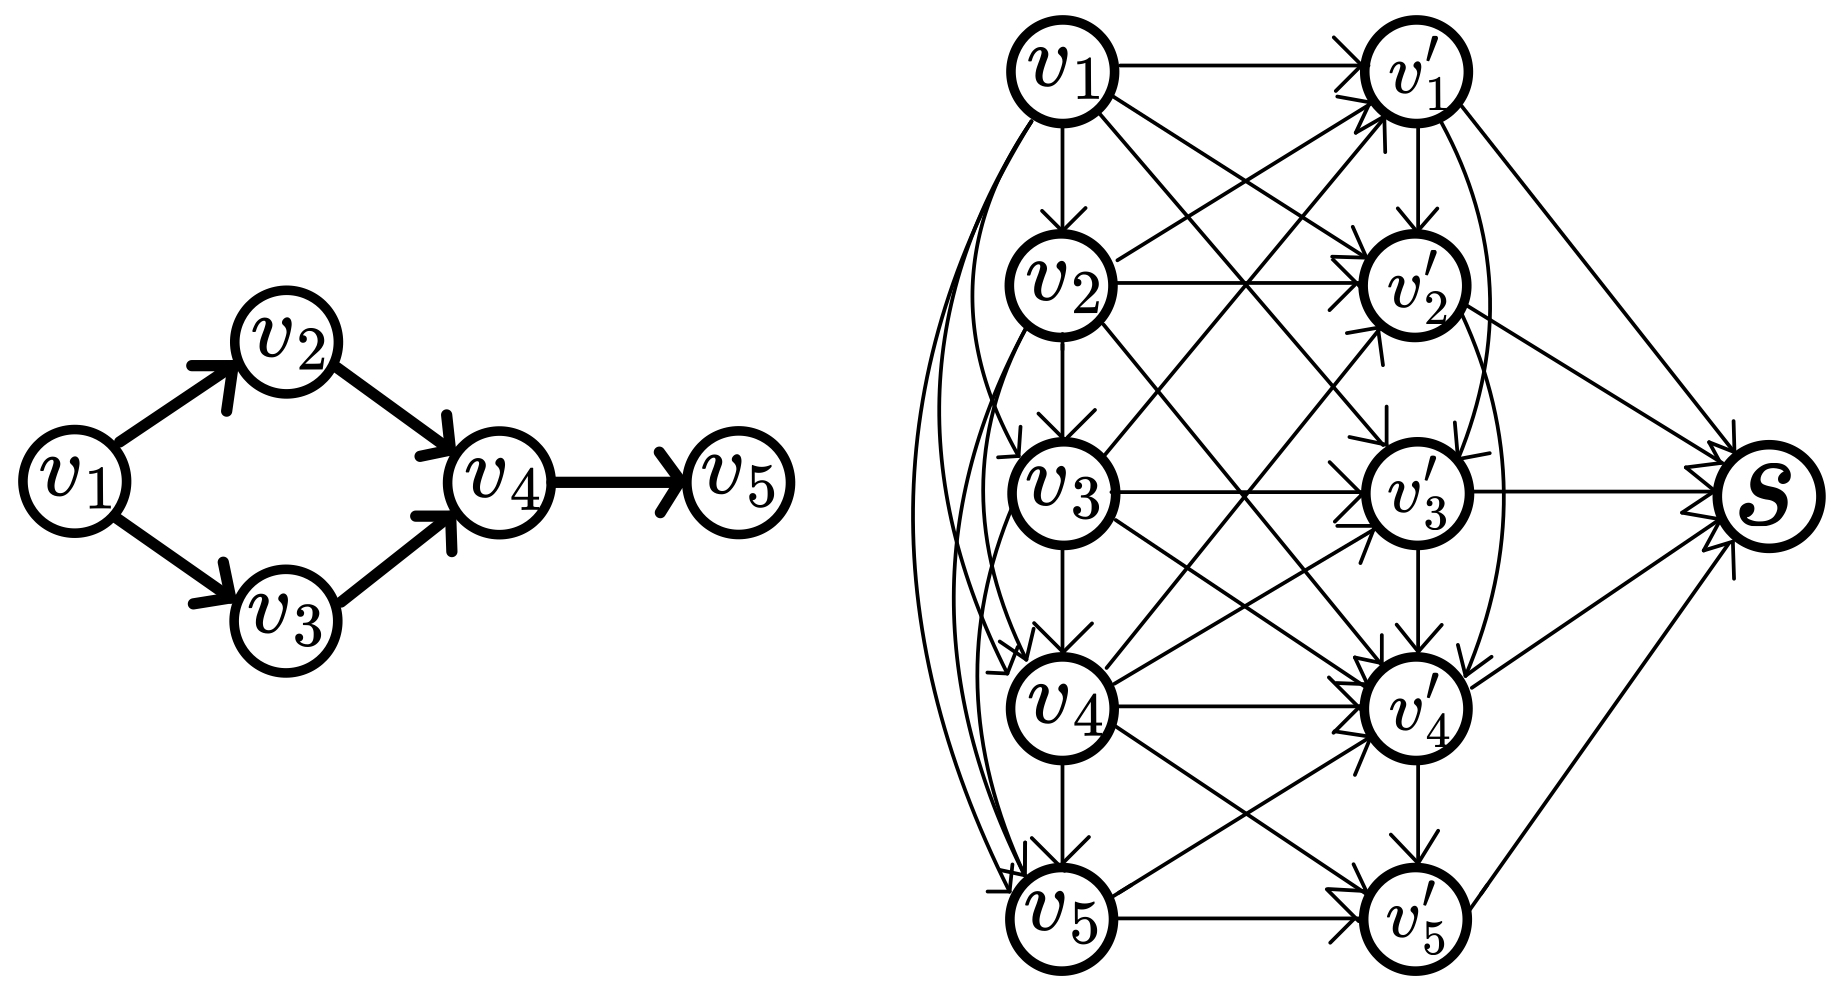
\includegraphics[width=15.0cm]{pic4.jpg}
        \caption{左の$G$から右の$G'$を構成した例.$G'$の頂点は$A = \{v_1, v_2, v_3, v_4, v_5\}, B = \{v'_1, v'_2, v'_3, v'_4, v'_5\}, \{s\}$からなる.$A$では任意の頂点対に枝があり,$B$では$G$と同じ枝の構成となっている.また$A, B$の間には$A$から$B$に向かう枝のみがあり,$B$の各頂点から$s$に向かう枝がある.}
        \label{fig:4}
    \end{figure}


    \begin{figure}[t]
        \centering
        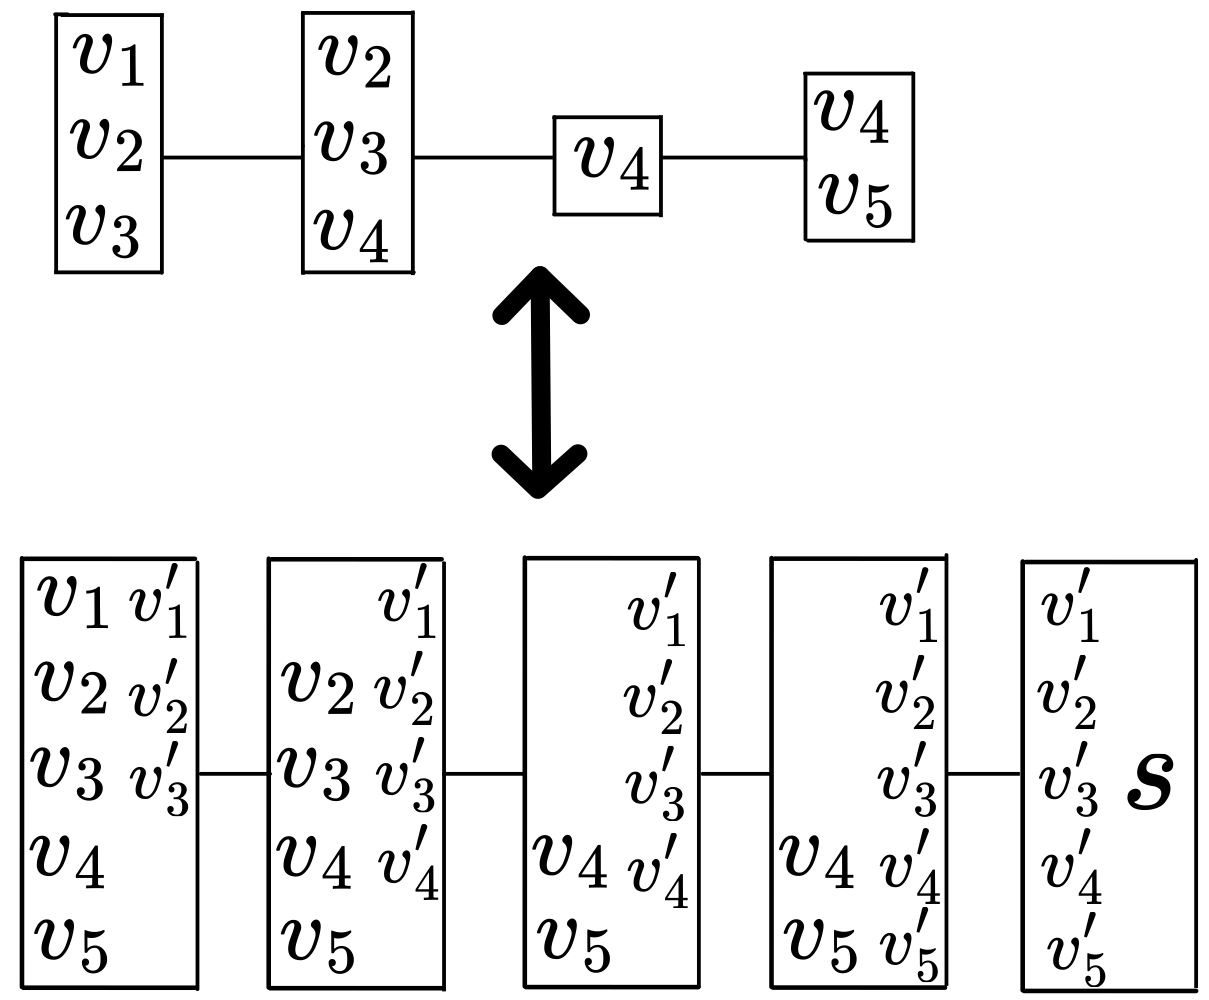
\includegraphics[width=10.0cm]{pic5.jpg}
        \caption{Figure★★\ref{fig:4}の$G, G'$に対するDAG-PD $(P, \beta),\ (P', \gamma)$ (それぞれ上,下)の構成例.$G$の頂点数を$n$とすると,$(P, \beta)$のwidthが$\mathsf{pw}(G)$のとき,$(P', \gamma)$のwidthは$\mathsf{pw}(G) + n$となる.}
        \label{fig:5}
    \end{figure}
    
    次に,widthが$\mathsf{pw}(G)$である$G$のDAG-PDを$(P, \beta)$ $(P = p_1, p_2, \dots, p_r)$とする.各$m$に対し,$G'$の頂点集合$\gamma(p_m)$を以下のように構成する.

    \vskip\baselineskip
    \begin{itemize}
        \item 各$(p_m)$に対し,$v \in \bigcup_{j = i}^{r} \beta(p_j)$ならば,$v$を$\gamma(p_m)$に加える.
        \item 各$(p_m)$に対し,$v \in \bigcup_{j = 1}^{i} \beta(p_j)$ならば,$v'$を$\gamma(p_m)$に加える.
    \end{itemize}

    さらに$\gamma(p_{r+1})$を下記のように定める.
    
    \vskip\baselineskip
    \begin{itemize}
        \item $\gamma(p_{r+1}) = B \cup \{s\}$
    \end{itemize}

    以上の操作によってできる$(P', \gamma)$ $(P' = p_1, p_2, \dots, p_{r+1})$が,$G'$のDAG-PDになっていることを示す.Figure★★\ref{fig:4}の$G, G'$に対するDAG-PD $(P, \beta),\ (P', \gamma)$の構成例をFigure★★\ref{fig:5}で示す.$\gamma$の構成法に注意すると,$\gamma(p_1)$は$A$の頂点をすべて含む.また$\gamma(p_{r+1})$は$B \cup \{s\}$を含む.よって$\sum_{m=1}^{r+1} \gamma(p_m) = V'$が成り立つため,$(P', \gamma)$はDAG-PDのルール1を満たす.また$\gamma$の構成法に注意すると,任意の$v \in V'$に対して,$v$を含む全てのバッグが$(p_1, P_2, \dots, p_r)$上で非連結になることはなく,また$\gamma(p_r)$は$B$の頂点をすべて含み,$s$は$\gamma(p_{r+1})$にのみ含まれるため,任意の$v \in V'$に対して,$v$を含む全てのバッグが$(p_1, P_2, \dots, p_r+1)$上で非連結になることはない.よって$(P', \gamma)$はDAG-PDのルール3を満たす.さらに,$(P', \gamma)$が$G'$の全ての枝に対してDAG-PDのルール2を満たすことを示す.$G'$上の各枝$e \in E'$を次の5つに場合分けして考える.なお,$v, v'$はそれぞれ$A, B$に含まれることに注意する.

    \begin{itemize}
        \item $e = (v_i, v_j)$ $(1 \leq i < j \leq n)$の場合:
        
        $A \subseteq \gamma(p_1)$より,$v_i, v_j \in \gamma(p_1)$
        \item $e = (v'_i, s)$ $(1 \leq i \leq n)$の場合:
        
        $B \cup \{s\} = \gamma(p_{r+1}), s \notin \gamma(p_r)$より,$v'_i, s \in \gamma(p_{r+1}), s \notin \gamma(p_r)$
        \item $e = (v_i, v'_i)$ $(1 \leq i \leq n)$の場合:
        
        $\gamma$の構成より,$v_i \in \beta(p_1)$ならば$v_i, v'_i \in \gamma(p_1)$.$v_i \notin \beta(p_1)$ならば,$(P, \beta)$で$v$が初めて現れたバッグを$\beta(p_m)$とすると,$v_i, v'_i \in \gamma(p_m)$であり,$v'_i$は$\gamma(p_1)$で初めて現れている.よって$v_i, v'_i \in \gamma(p_m), v'_i \notin \gamma(p_{m-1})$
        \item $e = (v_i, v'_j)$ $((v_i, v_j) \in E in G)$の場合:
        
        $\gamma$の構成より,$v_i, v_j \in \beta(p_1)$ならば$v_i, v'_j \in \gamma(p_1)$.$v_i, v_j \notin \beta(p_1)$ならば,$(P, \beta)$において,ある$m$があり,$v_i, v_j \in \beta(p_m), v_j \neq \beta(p_{m-1})$とできる.このとき,$\gamma$の構成より$v_i, v'_j \in \gamma(p_m), v'_j \notin \gamma(p_{m-1})$
        \item $e = (v_j, v'_i)$ $((v_i, v_j) \in E in G)$の場合:
        
        $(P, \beta)$において,$v_i$が初めて現れたバッグを$\beta(p_m)$とする.このとき$\gamma$の構成より,$v'_i$は$\gamma(p_m)$で初めて現れている.また$(P, \beta)$は$G$のDAG-PDであるから,ある$m'$があり,$v_i, v_j \in \beta(p_m'), v_j \neq \beta(p_{m'-1})$とできる.$\gamma$の構成より,$v_j \in \gamma(p_l)$ $(p_l = 1, 2, \dots, m')$がいえ,さらに$m \leq m'$に注意すると$v_j \in \gamma(p_m)$がいえる.したがって$v_j, v'_i \in \gamma(p_m), v_j \notin \gamma(p_{m-1})$
    \end{itemize}

    よって,$(P', \gamma)$はDAG-PDのルール2を満たす.以上より$(P', \gamma)$が$G'$のDAG-PDであることが示される.また,各$m = 1, 2, \dots, r$に対し,$v_i \in \beta(p_m)$ならば$v_i, v'_i \in \gamma(p_m)$であり,かつ$v_i \notin \beta(p_m)$ならば,$v_i, v'_i$のどちらか一方が$\gamma(p_m)$に含まれるため,$|\gamma(p_{r+1})| = n + 1$に注意すると,$(P', \gamma)$のwidthは$((P, \beta)$の$width)+ n$,すなわち$\mathsf{pw}(G) + n$であることがいえる.

    

    次に,$(P', \gamma)$が$G'$のDAG-PDのうち最小のwidthをもつDAG-PDであることを示す.$(P', \gamma)$よりもwidthの小さいDAG-PD $(Q, \delta)$ $(Q = (q_1, q_2, \dots, q_{r'}))$が存在すると仮定し,矛盾を導くことでこれを示す.まず,以下の手順によって$(Q, \delta)$と同じ幅をもつ$G'$のnice DAG-PDを構成する.

    \vskip\baselineskip
    \begin{enumerate}
        \item $(Q, \delta)$のバッグのうち,初めて$A$のすべての頂点が含まれたバッグを$\delta(q_i)$ $(q_i \in Q)$とする($A$の任意の2頂点間には枝があるため,このような$q_i$が存在することに注意する).ある$v' \in B$に対し,$v' \in \delta(q_j)$なる$q_j$ $(j < i)$が存在する場合,このような$q_j$を$Q$からすべて取り除く.$\delta(q_j) \subseteq \delta(q_i)$であったことに注意すると,$q_j$の削除後もwidthが同じ$G'$のDAG-PDになっており,こうしてできるDAG-PDを$(Q', \delta')$とする.
        \item $Q'$の左端に$q_0$ $(\delta'(q_0) = A)$を追加し,$(Q'', \delta'')$とする.
        \item $(Q'', \delta'')$のバッグのうち,初めて$B \cup \{s\}$のすべての頂点が含まれたバッグを$\delta''(q_k)$ $(q_k \in Q'')$とする($B$のすべての頂点から$S$に向かう枝があるため,このような$q_k$が存在することに注意する).$v \in \delta''(q_k)$なる$v \in A$が存在する場合,$Q''$から$\{q_j | j \geq k\}$をすべて取り除き,$q_{k-1}$の直後に,順に$q'_k, q'_{k+1}, q'_{k+2}$ $(\delta''(q'_k) = \delta(q_k) \backslash \{s\}, \delta''(q'_{k+1}) = B, \delta''(q'_{k+2}) = B \cup \{s\})$を追加する.この操作を行ってもDAG-PDのルールは満たされたままであり,かつwidthは操作前より大きくならないことに注意する.こうしてできるDAG-PDを$(Q''', \delta''')$とする.
        \item $(Q''', \delta''')$をwidthが同じnice DAG-PDに変換する.便宜上,このnice DAG-PDを$(Q, \delta)$ $(Q = (q_1, q_2, \dots, q_{r'})$と表記する.
    \end{enumerate}


    \begin{figure}[t]
        \centering
        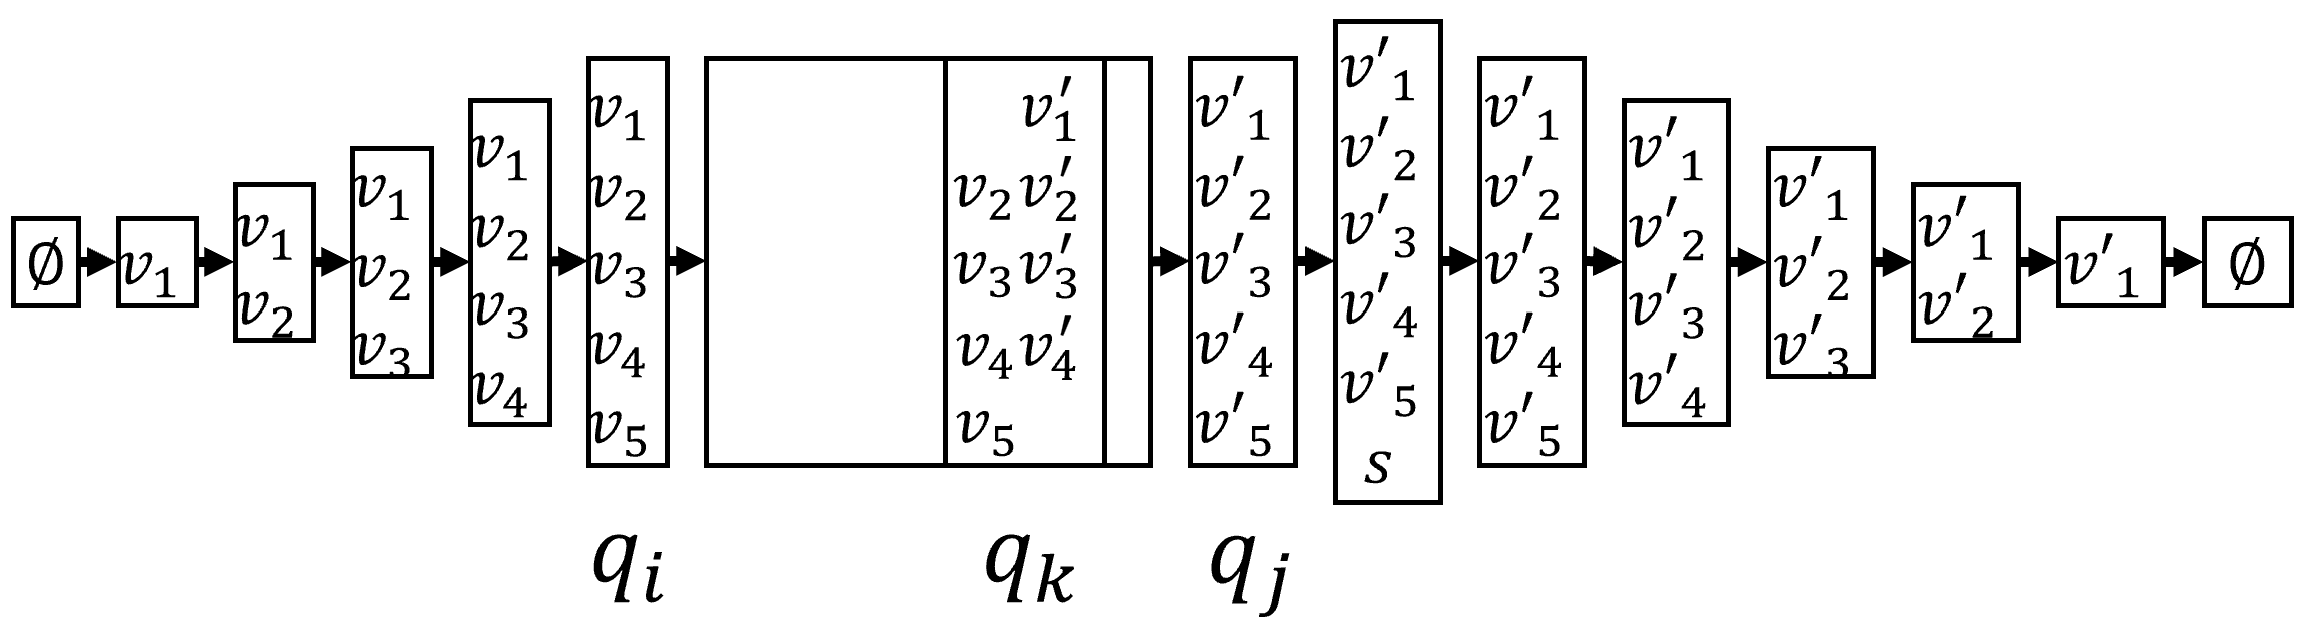
\includegraphics[width=15.0cm]{pic8.png}
        \caption{構成したnice DAG-PD $(Q, \delta)$の例.$q_i$で$A$の全ての頂点のintroduceが完了し,$q_j$で$B$の全ての頂点のintroduceが完了する.$q_i$と$q_j$の間のバッグ$q_k$では,各$i$に対して$v_i, v'_i$の少なくともどちらか一方が含まれる.}
        \label{fig:8}
    \end{figure}
    
    
    以上の操作によって構成されたnice DAG-PD $(Q, \delta)$は,はじめ$A$の頂点を順にintroduceし,ある$q_i$で$A$の全ての頂点のintroduceが終わった後,$B$の頂点のintroduceを行いつつ,$A$の頂点のfogetも行っていく.$B$のすべての頂点のintroduceが終わった後,ある$q_j$で$B$のみを含むバッグがあり,直後に$B \cup \{s\}$からなるバッグが続く.Figure★★\ref{fig:8}で構成後の例を示す.このとき,$\delta(q_k)$ $(q_k \in Q, i < k < j)$では,各$v_m, v'_m$ $(m = 1, 2, \dots, n)$について,$v_m, v'_m$の少なくともどちらか一方は$\delta(q_k)$に含まれる.なぜならば,$G'$には枝$(v_m, v'_m)$が存在し,$v_m, v'_m$を同時に含む$\delta(q_{i_m})$が存在すること,そして$\delta(q_i) = A, \delta(q_j) = B$に注意すると,$v_m \in \delta(q_{i_L}), v'_m \in \delta(q_{i_R})$ $(q_{i_L}, q_{i_R} \in Q, i \leq i_L \leq i_m \leq i_R \leq j)$がいえるからである.
    
    ここで各$m$ $(m = 1, 2, \dots, r')$に対し,$G$の頂点集合$\beta'(q_m)$を$\beta'(q_m) = \{v_i | \{v_i, v'_i\} \subseteq \delta(q_m) \}$と定める.このとき,$(Q, \beta')$が$G$のDAG-PDになっていることを示す.$G'$において任意の頂点対$(v, v')$ $(v \in A, v' \in B)$が隣接していることに注意すると,$(Q, \delta)$では$(v, v')$を同時に含むようなバッグが少なくとも1つ存在する.よって$\sum_{m=1}^{r'}\beta'(q_r') = V$が成り立つため,$(Q, \beta')$はDAG-PDのルール1を満たす.また$G'$のうち$B$によって誘導される部分グラフを$G'_B$とすると,$E(G'_B) = E(G)$であるため,$B$の頂点でintroduceされる順序は,$G'$の強連結成分に対するトポロジカル順序になる.したがって$(Q, \beta')$も$G'$の強連結成分がトポロジカル順序でintroduceされていくため,$(Q, \beta')$はDAG-PDのルール2を満たす.さらに,$(Q, \delta)$は$G'$のDAG-PDであるから,$(Q, \delta)$で$A$の頂点が一度forgetされた後,再びintroduceされることはない.よって$(Q, \delta)$で${v, v'}$を含むバッグが非連結になることはないため,$(Q, \beta')$でも$v$を含むバッグが非連結になることはない.したがってDAG-PDのルール3を満たす.

    以上より,$(Q, \beta')$は$G$のDAG-PDになっている.このとき,$(Q, \beta')$の各バッグは,$(Q, \delta)$の各バッグが$(v_i, v'_i)$を同時に含む場合のみ$v_i$を含んでいること,そして各$\delta(q_m)$には$v_i, v'_i$の少なくともどちらか一方が含まれることに注意すると,$(Q, \delta)$のwidth $k$に対し,$(Q, \beta')$のwidth $w_b$は高々$k - n$である.ここで仮定より$k < \mathsf{pw}(G) + n$であるため$w_b < \mathsf{pw}(G)$とできるが,これは$\mathsf{pw}(G)$が$G$のDAG-pathwidthであることと矛盾する.したがって仮定が誤りであり,$(P', \gamma)$が$G'$のDAG-PDのうち最小のwidthをもつDAG-PDであることが示される.
    
    以上より,$\mathsf{pw}(G') = \mathsf{pw}(G) + n$が導かれる.$G'$がsinkをただ1つもつこととLemma~\ref{sink}とより$\mathsf{tw}(G') = \mathsf{pw}(G')$がいえるため,$\mathsf{pw}(G') = \mathsf{tw}(G') = \mathsf{pw}(G) + n$が導かれる.
    
\end{proof}

\end{comment}





\subsection{co-DAG Tree Decomposition}
DAG-TD $T$をFPTアルゴリズムに利用する場合,$T$の葉から動的計画法を開始するとFPTを構築しやすい.本節では,よりFPTアルゴリズムの構築に適したDAG-TDであるco-DAG Tree Decompositionを定義する.


\begin{definition*}
 有向グラフ$G=(V, E)$のco-DAG Tree Decomposition (co-DAG-TD)とは,反有向木$T$と,$T$の各ノード$t$について$\beta(t) \subseteq V$であるような$\beta$とのペア$(T, \beta)$である.$(T, \beta)$は以下の3つを満たす.なお,$T$の根の数を$n_l$とする.
 
\begin{enumerate}
    \item $\sum_{t\in T} \beta(t) = V$ 
    \item $T$の各葉を$r_m$ $(m = 1, 2, \dots, n_r)$と表したとき,任意の枝 $ (u, v) \in E $ について以下の少なくともいずれか一方が成り立つ.
    \begin{itemize}
          \item ある$j$ $(1 \leq j \leq n_r)$があり,$u, v \in \beta(r_j)$
          \item ある$i$ $(i \in T)$とその親$j$があり,$u, v \in \beta(i)$, $u \notin \beta(j)$
    \end{itemize}
    \item 任意の$ i, j, k \in T$に対し,$j$が$i$から$k$までのパス上に存在するならば,$\beta(i) \cap \beta(k) \subseteq \beta(j)$.すなわち各$v \in V$について,$v$を含むバッグは$T$上で非空な部分反有向木を誘導する.
    \end{enumerate}
\end{definition*}

\begin{comment}
\begin{figure}[t]
    \centering
    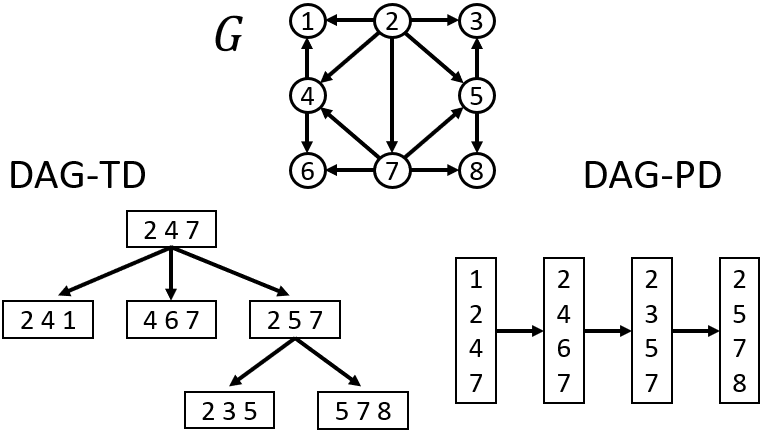
\includegraphics[width=15.0cm]{pic6.png}
    \caption{$G$に対するDAG-TDとDAG-PDの構成例.DAG-TD上での1つのパスは,$G$のある部分グラフに対するDAG-PDになっている.またDAG-PDもDAG-TDの一つであり,DAG-treewidthはDAG-Pathwidthより大きくならない.}
    \label{fig:6_2}
\end{figure}
\end{comment}

% co-DAG-TDの例をFigure★★\ref{fig:6_2}で示す.
以下でco-DAG-treewidthを定義する.

\begin{definition*}[co-DAG-treewidth]
    あるco-DAG-TD $(T, \beta)$のwidthを$\max_{t \in T}|\beta(t)|$と定義する.このとき,有向グラフ$G$のco-DAG-treewidth (co-DAG-treewidth)とは,$G$に対する全てのco-DAG-TDのうち,widthが最小であるco-DAG-TDのwidthである.
\end{definition*}

以降では,$G$のco-DAG-treewidthを$\mathsf{rtw}(G)$と表す.


\subsection{nice co-DAG-TD}

本節では,nice DAG-TDと同様にnice co-DAG-TD (nice co-DAG-TD)を説明する.

\begin{definition*}
 $G=(V, E)$を有向グラフとし,$(T, \beta)$を$G$のco-DAG-TDとする.$(T, \beta)$が以下の2つを満たすとき,$(T, \beta)$は$G$のnice co-DAG-TD (nice co-DAG-TD)であるという.
 
\begin{enumerate}
    \item $r_m$ $(m = 1, 2, \dots, n_r)$を$T$の各葉としたとき,全ての$m$に対して$\beta(r_m) = \varnothing$ 
    \item $R = \{r_m | m = 1, 2, \dots, n_r\}$としたとき,各$i \in T \backslash R$に対し,$\beta(i)$は以下のいずれかである.
    \begin{description}
          \item[introduce] $i$がただ1つの親$j$をもち,ある強連結成分$S$があり,$S \cap \beta(j) \neq \varnothing$かつ$\beta(i) = \beta(j) \cup S$
          \item[forget] $i$がただ1つの親$j$をもち,ある$v \in V$があり,$\beta(i) = \beta(j) \backslash \{v\}$
          \item[union] $i$がちょうど2つの親$j, k$をもち,$\beta(i) = \beta(j) = \beta(k)$
    \end{description}
    \end{enumerate}
\end{definition*}

\begin{comment}
\begin{figure}[t]
    \centering
    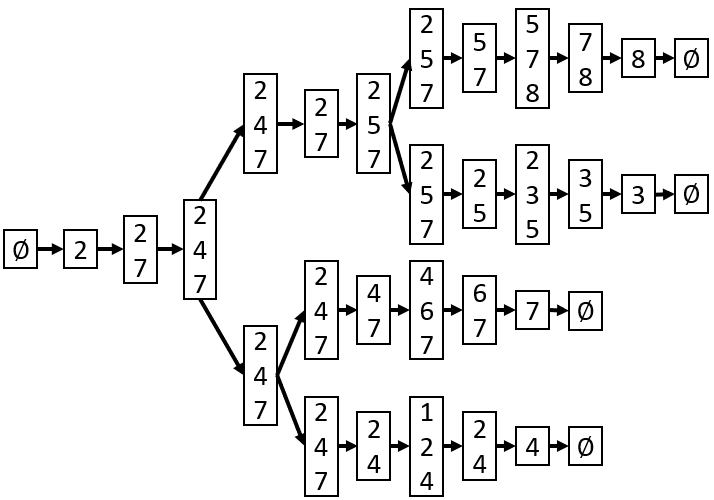
\includegraphics[width=15.0cm]{pic7.png}
    \caption{Figure★★\ref{fig:6}の$G$に対するnice DAG-TDの構成例.1つの根と複数のsinkをもち,それぞれ空集合からなる.それ以外のバッグは,親のバッグに対して強連結成分が1つ加えられたintroduceか,頂点が1つ除かれたforget,もしくは自身と同じ兄弟をもつunionのいずれかとなる.任意のDAG-TDから,同じwidthをもったnice DAG-TDを効率よく構築できる.}
    \label{fig:7}
\end{figure}
\end{comment}

% nice co-DAG-TDの例をFigure★★\ref{fig:7_2}で示す.
あるco-DAG-TDが与えられたとき,widthが同じである$G$のnice co-DAG-TDを効率よく構築することができる.

\begin{theorem}
    $(T, \beta)$が有向グラフ$G=(V, E)$のco-DAG-TDであるとする.また$(T, \beta)$のwidthを$w$とする.このとき,widthが$w$であるような$G$のnice co-DAG-TDを多項式時間で構築できる.
\end{theorem}

\begin{proof}
    $(T, \beta)$に対し,以下の手順を行いnice co-DAG-PDを得る.

    \begin{enumerate}
        \item $T$の各葉$r_m$に対し,親$r'_m$ $(\beta(r) = \varnothing)$を追加する.
        \item ある$i \in T$がただ1つの親$j \in T$をもち,かつ$\beta(i) = \beta(j)$ならば,$T$から$j$を除き,$j$のそれぞれの親から$i$への枝を加える.このような$i, j$がなくなるまでこの操作を繰り返す.
        \item 以下の5つの状態がなくなるまで操作を繰り返す.
        \begin{enumerate}
            \item ある$i \in T$と,その親$j \in T$について,$\beta(i) \nsubseteq \beta(j)$かつ$\beta(j) \nsubseteq \beta(i)$ならば,$i$と$j$の間に$i'$ $(\beta(i') = \beta(i) \cap \beta(j))$を加え,$(j, i', i)$の順につなぐ.
            \item ある$i \in T$と,その親$j \in T$について,$\beta(j) \subseteq \beta(i)$かつ$|\beta(i)| - |\beta(j)| \geq 2$ならば,$i$と$j$の間に$i''$ $(\beta(i'') = \beta(i) \backslash \{v\}, v \in \beta(i) \backslash \beta(j))$を加え,$(j, i'', i)$の順につなぐ.
            \item ある$i \in T$と,その親$j \in T$について,$\beta(i) \subseteq \beta(j)$かつ$\beta(j) \backslash \beta(i)$が強連結成分でないとき,$i$と$j$の間に$i'''$ $(\beta(i''') = \beta(j) \backslash A, A$は$\beta(j) \backslash \beta(i)$の強連結成分)を加え,$(j, i''', i)$の順につなぐ.
            \item ある$i$が$k$ $(k \geq 3)$個以上の親を持つとき,$i$の直前に,高さが$\lfloor \log_{2} k \rfloor$の完全二分反有向木$T'$ $(^{\forall}t' \in T'$について$\beta(t') = \beta(i))$を追加し,$T'$の各葉に対して2つずつ$i$の親を接続し,枝の向きは親から根への向きとする.ただし,$\lfloor x \rfloor$は$x$を超えない最大の整数値とする.
            \item ある$i$が2つの親$j, k$を持つとき,$i$と$j$,$i$と$k$の間にそれぞれ$j', k'$ $(\beta(j') = \beta(k') = \beta(i))$を追加し,それぞれ$(j, j', i),\ (k, k', i)$の順につなぐ.
        \end{enumerate}
    \end{enumerate}

    以上の操作によってできるco-DAG-TDは,widthが高々$w$であり,また$G$のnice co-DAG-TDである.この構築は$G$の頂点数の多項式時間で行える.
\end{proof}



\subsection{計算量クラス}

\begin{theorem}\label{r-NP困難}
    有向グラフ$G$が与えられたとき,$G$のco-DAG-treewidthを計算する問題はNP困難である.
\end{theorem}

Theorem~\ref{r-NP困難}の証明は付録で示す.

\begin{comment}
    
Theorem~\ref{r-NP困難}を証明するため,次で定義されるco-DAG-pathwidthの計算がNP困難であることを示す.


\begin{definition*}
     $G=(V, E)$とする.$G$のco-DAG Path Decomposition(co-DAG-PD)とは,以下の3つの条件をみたすようなVの各部分集合$ X_i (i = 1, 2,  \ldots, s)$の列 $X=(X_1, X_2,  \ldots, X_s)$ である.

    \begin{enumerate}
        \item $ X_1 \cup X_2 \cup \dots \cup X_s = V $ 
        \item 任意の有向枝 $ (u, v) \in E $ について,以下のいずれかが成り立つ.
        \begin{itemize}
            \item $u, v \in X_1$
        \item ある $i$ $(i \geq 2)$ があり,$u, v \in X_i$, $u \notin X_{i-1}$が成り立つ.
        \end{itemize}
        \item 任意の$ i, j, k\ (1 \leq i \leq j \leq k \leq s)$ について, $X_i \cap X_k \subseteq X_j$ が成り立つ.すなわち,各頂点$v$について,$v$は$X$上で非空な部分道を誘導する.
    \end{enumerate}
    あるco-DAG-PD $P = (X_1, X_2,   \ldots, X_s)$のwidthを$\max_{1 \leq i \leq s} {X_i}$と定義する.このとき,有向グラフ$G$のco-DAG-pathwidthとは,$G$に対する全てのco-DAG-PDのうち,widthが最小であるco-DAG-PDのwidthである.
    
\end{definition*}
 
以降では,$G$のco-DAG-pathwidthを$\mathsf{rpw}(G)$と表す.





\begin{lemma}\label{co-DAG-PD}
    有向グラフ$G$,整数$k$が与えられたとき,$\mathsf{rpw}(G) \leq k$が成り立つかを判定する問題はNP完全である.
\end{lemma}

\begin{proof}
    $G$のあるco-DAG-PDが与えられたとき,そのwidthが$k$以下かどうかを判定することは明らかに多項式時間で行えるため,この問題はNPに属する.また,$G$の全ての枝の向きを逆にした有向グラフを$G'$とする.$G$に対してwidthが$\mathsf{pw}(G)$であるDAG-PD $P$が与えられたとき,$G'$に対して最小のwidthをもつco-DAG-PD $P'$は,DAG-PDとco-DAG-PD定義より$P$と等しい.したがって$P'$のwidthは$\mathsf{pw}(G)$であるため,$\mathsf{rpw}(G')= \mathsf{pw}(G)$が成り立つ.以上よりLemma~\ref{co-DAG-PD}が示される.
\end{proof}





また,次のLemmaを示す.

\begin{lemma}\label{r-sink}
    $G =(V, E)$が$sink$をただ1つしか持たないならば,$\mathsf{rtw}(G) = \mathsf{rpw}(G)$が成り立つ.
\end{lemma}

\begin{proof}
    co-DAG-PD, co-DAG-TDの定義より,widthが$\mathsf{rpw}(G)$である$G$のco-DAG-PDは$G$のco-DAG-TDでもある.よって$\mathsf{rtw}(G) \leq \mathsf{rpw}(G)$が成り立つ.一方,widthが$\mathsf{rtw}(G)$である$G$のnice co-DAG-TDを$(T, \gamma)$とし,$G$のただ一つの強連結成分であるsinkを$A \subseteq V$とする.このときnice co-DAG-TDの定義より,ある根$r$とその子$r_c$があり,$\gamma(r) = \varnothing, \gamma(r_c) = A$が成り立つ.このとき$T$はただ一つの根$r$をもつことがいえる.なぜならば,もし$T$が$r$以外の根$r'$ $(\gamma(r') = \varnothing)$をもつと仮定すると,$r'$の子はバッグに$A$を含まないため,$G$に$A$以外のsinkが存在することになり,矛盾するからである.したがって$T$はunionのノードを持たず,任意の$t \in T$は入次数と出次数が高々1である.したがってco-DAG-PDとco-DAG-TDの定義より,$(T, \gamma)$は$G$のDAG-PDでもある.これより$\mathsf{rpw}(G) \leq \mathsf{rtw}(G)$がいえる.以上より,$\mathsf{rtw}(G) = \mathsf{rpw}(G)$が示される.
\end{proof}





最後にTheorem~\ref{r-NP困難}を示す.

\begin{proof}
    ある有向グラフ$G = (V, E)$が与えられたとき,定義\ref{NP困難}の証明と同様の手順で$|V'| = 2|V| + 1, |E'| = \frac{1}{2}(|V|^2 + 3|V|) + 2|E|$である有向グラフ$G' = (V', E')$ を構成する.また$G'$の頂点集合$A, B$を同様に$A = \{v_i | i =1, 2, \dots, n\}, B = \{v'_i | i =1, 2, \dots, n\}$と定める.このとき$V' = A \cup B \cup \{s\}$とできる.$G'$は$G$のサイズの多項式時間で構成できる.
    
    次に,widthが$\mathsf{rpw}(G)$である$G$のco-DAG-PDを$(P, \beta)$ $(P = p_1, p_2, \dots, p_r)$とする.各$m$に対し,$G'$の頂点集合$\gamma(p_m)$を以下のように構成する.

    \vskip\baselineskip
    \begin{itemize}
        \item 各$(p_m)$に対し,$v \in \bigcup_{j = i}^{r} \beta(p_j)$ならば,$v'$を$\gamma(p_m)$に加える.
        \item 各$(p_m)$に対し,$v \in \bigcup_{j = 1}^{i} \beta(p_j)$ならば,$v$を$\gamma(p_m)$に加える.
    \end{itemize}

    さらに$\gamma(p_0) = \gamma(p_1) \cup \{s\}$ $((p_0, p_1) \in E[T])$と定める.

    以上の操作によってできる$(P', \gamma)$ $(P' = (p_0, p_1, p_2, \dots, p_r))$が$G'$のco-DAG-PDになっていることを示す.Figure★★\ref{fig:4}の$G, G'$に対するco-DAG-PD $(P, \beta),\ (P', \gamma)$の構成例をFigure★★\ref{fig:5}で示す.$\gamma$の構成法に注意すると,$A \subseteq \gamma(p_r), B \subseteq \gamma(p_1)$がいえ,さらに$r \in \gamma(p_0)$であることから,$\sum_{m=0}^{r} \gamma(p_m) = V'$が成り立つ.よって$(P', \gamma)$はco-DAG-PDのルール1を満たす.また$\gamma$の構成法に注意すると,任意の$v \in V' \backslash \{r\}$に対して,$v$を含む全てのバッグが$(p_1, p_2, \dots, p_r)$上で非連結になることはなく,また$B \cup \{r\} \subseteq \gamma(p_0)$より,任意の$v \in V'$に対して,$v$を含む全てのバッグが$(p_0, p_1, p_2, \dots, p_r)$上で非連結になることはない.よって$(P', \gamma)$はco-DAG-PDのルール3を満たす.さらに定義\ref{NP困難}の証明と同様の議論により,$(P', \gamma)$がco-DAG-PDのルール2を満たすことがいえる.以上より$(P', \gamma)$は$G'$のco-DAG-PDである.このとき$(P', \gamma)$の幅は$\mathsf{rpw}(G)+n$である.

    さらに\ref{NP困難}の証明と全く同様の議論により,$(P', \gamma)$が$G'$に対してwidthが最小のco-DAG-PDであることがいえる.ここで$G'$はsinkを一つしか持たないことに注意すると,Lemma~\ref{r-sink}より$\mathsf{rtw}(G') = \mathsf{rpw}(G')$がいえ,$\mathsf{rtw}(G) = \mathsf{rpw}(G) + n$が成り立つ.以上より定義\ref{r-NP困難}が示される.
\end{proof}

\end{comment}

















\section{co-DAG-treewidthを用いたFPTアルゴリズム} %\label{sec_HowToUseTreewidth}

\subsection{Directed Dominating Set Problemの$O(2^ww^2n)$時間アルゴリズム}

以下では,頂点数$n$のDAG $G$と幅が$w$である$G$のco-DAG-TDが与えられたときに,$G$のDirected Dominating Set Problemを$O(2^ww^2n)$で計算するアルゴリズムを示す.


\begin{theorem}
    DAG $G$に対し,幅が$w$である$G$のnice co-DAG-TDが与えられたとき,$G$のDiDS problemを$O(2^ww^2n)$で解くアルゴリズムが存在する.
\end{theorem}

\vskip\baselineskip
上記のアルゴリズムを構成するため,まず関数$\mathsf{DS}$を定義する.

\begin{definition*}[$\mathsf{DS}$]
    DAG $G=(V, E)$のnice co-DAG-TDを$(T, \beta)$とし,その幅を$w$とする.ある$i \in T$に対し,頂点集合$A_i, B_i \subseteq V$が$A_i \cup B_i = \beta(i), A_i \cap B_i = \varnothing$を満たすとする.$G_i$を頂点集合$\bigcup_{k} \beta(k)$ ($k$は$i$を根とする$T$の部分反有向木のノード)によって誘導される$G$の部分グラフとする.関数$\mathsf{DS}$を以下のように定める.
    %
    \begin{equation}\label{def_ds2}
        \mathsf{DS}(i, A_i, B_i) = (\min |S_i|, D)
    \end{equation}

    ただし$S_i \subseteq V[G_i]$, $D \subseteq B_i$を満たし,$D$が支配されれば$S_i$は$G_i$のminimum-DiDSであり,かつ$A_i \subseteq S_i$, $B_i \cap S_i = \varnothing$を満たすとする.
\end{definition*}

%\vskip\baselineskip
以下で$\mathsf{DS}$の計算式を与える.各$\beta(i)$がintroduce, forget, unionのいずれかで場合分けをして計算する.
%
\begin{align*}
    \intertext{$\bullet$ $i$がただ一つの親$j$をもち,かつ$\beta(i)$が$v \in V$をintroduceしているとき}
    &\mathsf{DS}(i, A_i, B_i) = 
    \begin{cases}
        (\mathsf{DS}(j, A_i \backslash \{v\}, B_i)[0]+1, \mathsf{DS}(j, A_i \backslash \{v\}, B_i)[1] \backslash \mathsf{suc}(v)) &(v \in A_i) \\
        (\mathsf{DS}(j, A_i, B_i \backslash \{v\})[0], \mathsf{DS}(j, A_i, B_i \backslash \{v\})[1] \cup \mathsf{suc}(v)) &(v \in B_i)
    \end{cases}
    \intertext{$\bullet$ $i$がただ一つの親$j$をもち,かつ$X_i$が$v \in V$をforgetしているとき}
    &\mathsf{DS}(i, A_i, B_i) = 
    \begin{cases}
        (\mathsf{DS}(j, A_i \cup \{v\}, B_i)[0], \mathsf{DS}(j, A_i \cup \{v\}, B_i)[1]) &(v \in \mathsf{DS}(j, A_i, B_i \cup \{v\})[1]) \\
        (\mathsf{DS}(j, A_i, B_i \cup \{v\})[0], \mathsf{DS}(j, A_i, B_i \cup \{v\})[1]) &(otherwise)
    \end{cases}
    \intertext{$\bullet$ $i$が二つの親$j, k$をもつとき}
    &\mathsf{DS}(i, A_i, B_i) = 
    (\mathsf{DS}(j, A_i, B_i)[0] + \mathsf{DS}(k, A_i, B_i)[0] - |A_i|, \mathsf{DS}(j, A_i, B_i)[1] \cap \mathsf{DS}(k, A_i, B_i)[1])
\end{align*}

$\mathsf{DS}$を用いて,DAG $G$のnice co-DAG-TD $(T, \beta)$が与えられたときに,$G$のmDiDSのサイズを出力するアルゴリズム$\mathsf{Compute}$を示す.

%\vskip\baselineskip

$\mathsf{Compute}(T, \beta)$

\begin{enumerate}
    \item First Step: $T$の各根$r$に対し,$\mathsf{DS}(r, \varnothing, \varnothing) = (0, \varnothing)$とする.
    \item Exection Step: 各バッグ$\beta(i)$に対し,$A_i, B_i$全ての組合せについて各根から順に$\mathsf{DS}(i, A_i, B_i)$を計算する.
    \item Final Step: $i$が$T$のただ一つの葉$l$となったとき,$\mathsf{DS}(l, \varnothing, \varnothing)[0]$を出力する.
\end{enumerate}


\begin{lemma}\label{dids2}
    $\mathsf{Compute}$は$G$のmDiDSのサイズを返す.
\end{lemma}

\ref{dids2}の証明は付録で示す.

\begin{comment}
    
\begin{proof}
    $i=l$のとき,定義\ref{def_ds2}より$DS$はmDiDSのサイズを出力する.したがって各$i \in T$に対し,$DS(i, A_i, B_i)$が$DS$の定義\ref{def_ds}を満たすことを示せば十分.これを$i$に関する数学的帰納法で示す.
    まず$i$が$T$の根のとき$\beta(i) = \varnothing$であり,First Stepより明らかに定義\ref{def_ds2}を満たす.
    次にある$i$での定義\ref{def_ds2}の成立を仮定する.以下で$i$の子$i'$がintroduceかforgetかunionかで場合分けを行う.
    \begin{itemize}
        \item $i'$が$v \in V$をintroduceする場合 \\
        $i'$はただ一つの親$i$をもつ.$v \in A_{i'}$の場合,co-DAG-TDのルール2より$v$の後続頂点は$i'$の時点で全てintroduceされており,$v$は$\mathsf{suc}(v)$を支配する.またco-DAG-TDのルール2より$v$は$i'$の時点でどの頂点からも支配されていない.仮定より$D = DS(i, A_{i'}, B_{i'})[1]$が支配されれば$G_i$のmDiDSのサイズは$DS(i, A_{i'}, B_{i'})[0]$であるから,$D \backslash \mathsf{suc}(v)$が支配されれば$G_{i'}$のmDiDSのサイズは$DS(i, A_{i'}, B_{i'})[0] + |v|$となる.したがって$i'$でも定義\ref{def_ds2}を満たす.

        $v \in B_{i'}$の場合,$v$は支配集合に含まれないので$i'$以降にintroduceされる頂点によって支配される必要がある.仮定より$D = DS(i, A_{i'}, B_{i'})[1]$が支配されれば$G_i$のmDiDSのサイズは$DS(i, A_{i'}, B_{i'})[0]$であるから,$D \cup \{v\}$が支配されれば$G_{i'}$のmDiDSのサイズは$DS(i, A_{i'}, B_{i'})[0]$となる.したがって$i'$でも定義\ref{def_ds2}を満たす.
        
        \item $i'$が$v \in V$をforgetする場合 \\
        $i'$はただ一つの親$i$をもつ.$v \in DS(i, A_{i'}, B_{i'} \cup \{v\})[1]$の場合,$v$を支配する頂点は$A_{i'}$に存在しないため,$i$の時点で$v$自身が支配集合に含まれている必要がある.逆にこのとき,仮定より$DS(i, A_{i'} \cup \{v\}, B_{i'})[1]$が支配されれば$G_i$のmDiDSのサイズは$DS(i, A_{i'} \cup \{v\}, B_{i'})[0]$であるため,$i'$でも定義\ref{def_ds2}を満たす.

        $v \notin DS(i, A_{i'}, B_{i'} \cup \{v\})[1]$の場合,$v$を支配する頂点が$A_{i'}$に少なくとも1つ存在する.したがって$v$は$i$の時点で$A_{i'}, B_{i'}$のいずれに含まれていてもよく,またmDiDSのサイズが小さくなるのは$v$が$B_{i'}$に含まれている場合である.仮定より$DS(i, A_{i'}, B_{i'} \cup \{v\})[1]$が支配されれば$G_i$のmDiDSのサイズは$DS(i, A_{i'}, B_{i'} \cup \{v\})[0]$であるため,$i'$でも定義\ref{def_ds2}を満たす.

        \item $i'$が二つの親$i, \overline{i}$をもつunionであるとき \\
        $\overline{i}$においても定義\ref{def_ds2}が成立していると仮定する.また$D_i = DS(i, A_i, B_i)[1], D_{\overline{i}} = DS(\overline{i}, A_{\overline{i}}, B_{\overline{i}})[1]$とする.以下では$A_{i'} = A_{i} = A_{\overline{i}}, B_{i'} = B_{i} = B_{\overline{i}}$であることに注意する.$D_i = D_{\overline{i}}$の場合,仮定より$D_i$が支配されれば$S_i$は$G_i$のmDiDSであり,かつ$D_i$が支配されれば$S_{\overline{i}}$は$G_{\overline{i}}$のmDiDSである.このとき$S_{i} \cap S_{\overline{i}} = A_{i'}$が成り立つ.なぜならば定義\ref{def_ds2}より$B_{i} \cap S_i = \varnothing, B_{\overline{i}} \cap S_{\overline{i}} = \varnothing$であり,co-DAG-TDのルール3より任意の$s \in S_{i} \cap S_{\overline{i}}$を含むバッグは$T$上で$i', i, \overline{i}$を含む連結な反有向木を形成しているからである.したがって$V[G_{i'}] = V[G_i] \cup V[G_{\overline{i}}]$に注意すると,$D_i$が支配されれば$S_i \cup S_{\overline{i}}$は明らかに$G_{i'}$のmDiDSである.このときmDiDSのサイズは$DS(i, A_{i'}, B_{i'})[0] + DS(\overline{i}, A_{i'}, B_{i'})[0] - |A_{i'}|$であるため$i'$でも定義\ref{def_ds2}を満たす.

        $D_i \neq D_{\overline{i}}$の場合,$D_{\overline{i}} \backslash D_i \neq \varnothing$としても一般性を失わない.このときある頂点$w \in D_{\overline{i}} \backslash D_i$が存在する.定義\ref{def_ds2}より$w$は$B_{\overline{i}} = B_{i} = B_{i'}$に含まれ,かつ$w$はある頂点$w' \in S_i\subseteq V[G_i]$によって支配されており,$S_{\overline{i}}$には$w$を支配する頂点が存在しない.ここで$V[G_{i'}] = V[G_i] \cup V[G_{\overline{i}}]$であるから,$S_{i'} = S_i \cup S_{\overline{i}}$とすることで$S_{i'}$には$w$を支配する$w'$が含まれる.したがって仮定に注意して$D_i \cap D_{\overline{i}}$が支配されれば$S_i \cup S_{\overline{i}}$は明らかに$G_{i'}$のmDiDSである.上記と同様の議論により$|S_i \cup S_{\overline{i}}| = DS(i, A_{i'}, B_{i'})[0] + DS(\overline{i}, A_{i'}, B_{i'})[0] - |A_{i'}|$であるため,$i'$においても定義\ref{def_ds2}を満たす.
        
    \end{itemize}
    以上より,$i'$でも定義\ref{def_ds2}が成立.数学的帰納法によりLemma~\ref{dids2}が証明された.
\end{proof}

\end{comment}

最後に$\mathsf{Compute}$の計算量を示す.

\begin{lemma}
    DAG $G$の頂点数が$n$であるとする.このとき,幅が$w$である$G$のco-DAG-TD $(T, \beta)$が与えられたとき,$\mathsf{Compute}(T, \beta)$は$O(2^ww^2n)$の計算時間で結果を出力する.
\end{lemma}

\begin{proof}
    各バッグ$\beta(i)$に対し,$|\beta(i)| \leq w+1$に注意すると,$A, B$の組合せは高々$2^{w+1}$通り存在する.また$(T, \beta)$のバッグ数は高々$O(wn)$である.さらにintroduce, forget, unionのそれぞれでの計算と条件の判定は高々$O(w)$時間を要する.以上より,$\mathsf{Compute}$の計算量は$O(2^ww^2n)$である.
\end{proof}





















\section{結論} %\label{sec-conclusion}
本章では本研究のまとめと今後の課題を示す.本研究では次の3つを行った.

まず1つ目にDAGパス幅をパラメータとして有向支配集合問題,最大葉分岐問題,$k$-有向点素パス問題,有向シュタイナー木問題を解くアルゴリズムを構築した.前提として入力グラフのパス分解がすでに与えられているとし,バッグがintroduceかforgetかで場合分けを行っている.これにより幅が$w$であるDAGパス分解を入力したときにそれぞれ$O(2^w w n)$, $O(2^w w n + n^2)$, $O((k+1)^w(w^2+k)n+n^2)$, $O(2^w (k + w)n + n^2)$で計算できることを示した.

2つ目にDAGパス分解を求める近似アルゴリズム及びパラメータ化アルゴリズムを構築した.近似アルゴリズムでは,DAG上のセパレータを利用した分割統治法を用いることで$O(\log^2 n)$-近似のアルゴリズムを構築した.またDAG上でのDAGパス分解の構築が\textit{one-shot Black Pebbling}問題と等価であることを示し,近似比がより小さい$O(\log^{2/3} n)$-近似アルゴリズムの存在も示した.さらに入力DAGの最大出次数を$d$,根数を$l$としたとき,入力整数$k$に対して幅が高々$O(ld^k)$のDAGパス分解を出力するか,DAGパス幅が$k$より大きいことの証拠を示すアルゴリズムを構築した.このアルゴリズムは完全有向$d$分木の埋め込みを利用して設計したもので,出次数が制限されたDAGに対して効率的にDAGパス分解を構築できることを初めて示した.

3つ目にDAGパス幅を拡張する概念としてDAG木幅を提案した.DAG木幅は有向グラフがどれだけ有向木に近い構造を持つかを表すパラメータであり,DAGパス幅より大きくならず,同様の手法でアルゴリズムを構築できる点が利点である.本論文ではDAG木幅を用いて有向支配集合問題を解く$O(2^w w n)$時間アルゴリズムを構築した.これによりDAGパス幅を用いたアルゴリズムと比較して計算速度の向上を実現した.

最後に今後の課題として2点挙げる.1つ目は$O(ld^k)$の幅を持つDAGパス分解を出力するアルゴリズムにおいて幅の値を小さくすることである.特に最大出次数$d$は頂点数$n$まで増大する可能性があるため,これを定数にまで抑える方法を検討したい.2つ目はDAGパス分解アルゴリズムを有向グラフ全体に拡張することである.本研究でのアルゴリズムはDAGに限定されているが,DAGパス幅自体は一般の有向グラフに対して定義されているため,幅の小さなDAGパス分解を一般の有向グラフに対しても適用できるようにする余地がある.
















\acknowledgments				% 謝辞
最後に,本研究にあたって様々な助力をしていただいた指導教員である川原純准教授及び湊真一教授や岩政勇仁助教など湊研究室の方々に深謝いたします.また,私生活の面で20年以上にもわたって支えていただいた両親に感謝します.


\begin{comment}
残り:\\
・タイトル→OK!\\
・abstract→OK!\\
・introduction→OK!\\
・結論→OK!\\
・bib→OK!\\
・付録に回す箇所→OK!\\
・図★★\\
    
\end{comment}






\nocite{*}
\bibliographystyle{kuisunsrt}			% 文献スタイルの指定
\bibliography{main}				% 参考文献の出力








						% 付録の開始
\Appendix[付録]



\section{\ref{lob}の証明}
   
\begin{proof}
    以下では$\mathsf{Compute}$のPreprocesingを行ったあとの場合を考える.すなわちグラフ$G$,nice DAG-PDは根$r$から到達可能な頂点のみが現れるものとする.また$\mathsf{Compute}$のFirst Stepより,$G$が根$r$のみからなる場合は1を出力するためMaxLOBの解となっている.以下では$G$に根$r$以外の頂点も含まれる場合を考える.Lemma~\ref{lob}の証明は,各$i$に対し$\mathsf{LOB}(i, A_i, B_i)$が$\mathsf{LOB}$の定義\ref{def_lob}を満たすことを示せば十分.これを$i$に関する数学的帰納法で示す.以下では便宜上,木を成す頂点のうち葉以外の頂点を茎と呼ぶ.\\
    $i=1$のとき,$\mathsf{Compute}$のFirst Stepより$\mathsf{LOB}(1, \{r\}, \varnothing) = -\infty, \mathsf{LOB}(1, \varnothing, \{r\}) = 0$である.根$r$は葉となり得ないことに注意すると明らかに定義\ref{def_lob}を満たす.\\
    $i=k$のとき,$\mathsf{LOB}(i, A_i, B_i)$が定義\ref{def_lob}を満たすと仮定する.以下で$X_{k+1}$が$v \in V$をintroduceするかforgetするかで場合分けを行う.
    \begin{itemize}
        \item $X_{k+1}$が$v \in V$をintroduceする場合 \\
        $v \in A_{k+1}$の場合,DAG-PDのルール2より$\mathsf{pred}(v) \subseteq (A_{k+1} \cup B_{k+1})$である.$B_{k+1}$は有向全域木の茎を表すことに注意すると,ある茎$u \in \mathsf{pred}(v) \cap B_{k+1}$が存在する場合に限り$v$を葉とすることができる.仮定より$G_k$において$\mathsf{LOB}(k, A_{k+1} \backslash \{v\}, B_{k+1})$は,$A_{k+1} \backslash \{v\}$を葉集合,$B_{k+1}$を茎集合とする葉数最大の有向全域木であり,これに$v$を葉として加えることで葉数を1だけ大きくできる.したがって$\mathsf{LOB}(k+1, A_{k+1} \backslash \{v\}, B_{k+1})+1$は$A_{k+1}$を葉集合,$B_{k+1}$を茎集合とする有向全域木の葉数の最大値を表す.逆にこのような茎$u$が存在しなければ$v$は葉とならないため,値を$-\infty$とすることで解にならないことを表す.以上より$v \in A_{k+1}$の場合は定義\ref{def_lob}を満たす.\\
        $b \in B_{k+1}$の場合も同様の議論により定義\ref{def_lob}を満たす.ただし$v$は茎であるため$\mathsf{LOB}$の値は大きくならないことに注意する.

        \item $X_{k+1}$が$v \in V$をforgetする場合 \\
        葉数がそれぞれ$\mathsf{LOB}(k, A_{K+1} \cup \{v\}, B_{k+1}), \mathsf{LOB}(k, A_{k+1}, B_{k+1} \cup \{v\})$である有向全域木を$T^A_k, T^B_k$と表す.まず$\mathsf{LOB}(k, A_{K+1} \cup \{v\}, B_{k+1}) \geq \\\mathsf{LOB}(k, A_{k+1}, B_{k+1} \cup \{v\})$の場合,$v$が葉であるような$T^A_k$が実際に存在することを示す.このとき$\mathsf{LOB}(k, A_{K+1} \cup \{v\}, B_{k+1}) \neq -\infty$であるため,$v$をintroduceしたバッグを$X_j$とすると,$i=j$における$\mathsf{LOB}$の値も$-\infty$でない.したがって式\ref{intro_lob}の第一式の条件より,$i=j$において$v$が葉であるような有向全域木の存在が保証される.$X_m$ $(j < m < k+1)$において$v$はintroduceもforgetもされないことに注意すると,$T^A_k$は実際に$v$を葉として含むことが示される.次に$\mathsf{LOB}(k, A_{K+1} \cup \{v\}, B_{k+1}) < \mathsf{LOB}(k, A_{k+1}, B_{k+1} \cup \{v\})$の場合,$v$が茎であるような$T^B_k$が実際に存在することを示す.上記と同様の議論により,$T^B_k$には$v$の先行頂点が必ず存在する.また$T^B_k$において$v$と共通の子をもつ頂点も存在しない.なぜならば,もしそのような頂点$v'$ (ある$w \in V[T^B_k]$があり,$\{(v, w),\ (v', w)\} \subseteq E[T^B_k]$)が存在したとすると,$T^B_k$において$v$に$w$以外の子が存在するならば,新たに$T^B_k = (V[T^B_k], E[T^B_k] \backslash \{(v, w)\})$とすることで$v$と$v'$が共通の子を持たないようにすることができる.この操作を繰り返すことで$v$と共通の子をもつ頂点が存在しないような有向全域木を構築できる.$T^B_k$において$v$に$w$以外の子が存在しないならば,$E[T^B_k]$から$(v, w)$を除くことで$v$を葉とする有向全域木$T^A_k$が構築できる.このとき明らかに$|\mathsf{Leaf}(T^A_k)| = |\mathsf{Leaf}(T^B_k)| + 1$であるが,これは$\mathsf{LOB}(k, A_{K+1} \cup \{v\}, B_{k+1}) < \mathsf{LOB}(k, A_{k+1}, B_{k+1} \cup \{v\})$と矛盾する.したがって$T^B_k$において$v$と共通の子をもつ頂点は存在せず,$v$が実際に茎であるような$T^B_k$が存在することが示される.\\
        ここで$G_{k+1} = G_k$より,$G_{k+1}$の有向全域木の最大葉数は$G_k$のそれと等しい.したがって$v$を葉に含むような$G_k$の有向全域木の最大葉数と,$v$を茎に含むような$G_k$の有向全域木の最大葉数のうち,より大きい方を$G_{k+1}$の有向全域木の最大葉数とすることができる.仮定より,それぞれ$\mathsf{LOB}(i, A_{i+1} \cup \{v\}, B_{i+1}), \mathsf{LOB}(i, A_{i+1}, B_{i+1} \cup \{v\})$と表すことができるため,$\max \{\mathsf{LOB}(i, A_{i+1} \cup \{v\}, B_{i+1}), \mathsf{LOB}(i, A_{i+1}, B_{i+1} \cup \{v\})\}$は$G_{k+1}$の有向全域木の最大葉数と等しい.したがって定義\ref{def_lob}が成立.
    \end{itemize}
    以上より,$i = k+1$でも定義\ref{def_lob}が成立.数学的帰納法によりLemma~\ref{lob}が証明された.
\end{proof}



















\section{Theorem~\ref{NP困難}の証明}
Theorem~\ref{NP困難}を証明するため以下のLemmaを示す.

\begin{lemma}\label{sink}
    有向グラフ$G=(V, E)$の強連結成分$A$があり,$A$から$V \backslash A$への枝が存在しないとき,$A$を$G$の$sink$と呼ぶ.このとき,$G$が$sink$をただ1つしか持たないならば,$\mathsf{tw}(G) = \mathsf{pw}(G)$が成り立つ.
\end{lemma}


\begin{proof}
    DAG-PD, DAG-TDの定義より,widthが$\mathsf{pw}(G)$である$G$のDAG-PDは$G$のDAG-TDでもある.よって$\mathsf{tw}(G) \leq \mathsf{pw}(G)$が成り立つ.一方,widthが$\mathsf{tw}(G)$である$G$のnice DAG-TDを$(T, \gamma)$とし,sink$A$を含む$T$のバッグのうち,根$r \in T$からの距離が最も近いものを$\gamma(t_i)$ $(t_i \in T)$とする.$T$上で$r$から$t_i$までのパスを$P \subseteq T$としたとき,$(P, \gamma)$が$G$のDAG-PDとなっていることを示す.まず,$P$について$\sum_{p \in P} \gamma(p) = V$が成り立つ.なぜならば,$T$上で$P$に含まれない$P'$があり,かつ任意の$p \in P$に対し,$P'$上で,ある$v \notin \gamma(p)$がintroduceされたとすると,頂点集合$\sum_{p' \in P'} \gamma(p')$が誘導する$G$の部分有向グラフはあるsink$A'$をもつが,$p_A \in P$ $(A \subseteq \gamma(p_A))$と$p_{A'} \in P'$ $(A \subseteq \gamma(p_{A'}))$は非連結であるから,DAG-TDの定義より,$A \neq A'$である.これは$G$がsinkをただ1つしかもたないことと矛盾する.したがって$\sum_{p \in P} \gamma(p) = V$が成り立つことがいえ,$(P, \gamma)$はDAG-PDのルール1を満たす.またDAG-TDのルール2と,$P$がパスであることから$(P, \gamma)$はDAG-PDのルール2を満たす.さらに$P$はパスであるからルール3も満たす.よって$(P, \gamma)$は$G$のDAG-PDである.したがって$\mathsf{pw}(G) \leq \mathsf{tw}(G)$がいえる.以上より,$\mathsf{tw}(G) = \mathsf{pw}(G)$が示される.
\end{proof}


上のLemmaを用い,[3]の手法を参考にしてTheorem~\ref{NP困難}を示す.

\begin{proof}[proof of Theorem~\ref{NP困難}]
    ある有向グラフ$G = (V, E)$が与えられたとき,以下の手順で有向グラフ$G' = (V', E')$ $(|V'| = 2|V| + 1, |E'| = \frac{1}{2}(|V|^2 + 3|V|) + 2|E|)$を構成する.

    \vskip\baselineskip
    \begin{itemize}
        \item $V = \{v_i | i = 1, 2, \dots, n\}$としたとき,$V' = \{v_i, v'_{i} | i = 1, 2, \dots, n\} \cup \{s\}$とする.
        \item $(v_i, v_j)$ $(v_i, v_u \in V', 1 \leq i < j \leq n)$の全ての組合せに対し,$(v_i, v_j) \in E'$とする.
        \item 各$i$ $(i = 1, 2, \dots, n)$に対し,$(v_i, v'_i),\ (v'_i, s) \in E'$とする.
        \item $v_p, v_q \in V$ について$(v_p, v_q) \in E$であるならば,$(v_p, v'_q),\ (v_q, v'_p),\ (v'_p, v'_q) \in E'$とする.
    \end{itemize}
    
    以上の操作によってできる有向グラフを$G'$とする.$G'$の構成例をFigure\ref{fig:4}に示す.$G'$は$G$のサイズの多項式時間で構成できる.また$G'$の頂点集合$A, B$を,$A = \{v_i | i =1, 2, \dots, n\}, B = \{v'_i | i =1, 2, \dots, n\}$と定める.このとき$V' = A \cup B \cup \{s\}$とできる.


\ifthenelse{\boolean{Draft}}{
    \begin{figure}[t]
        \centering
        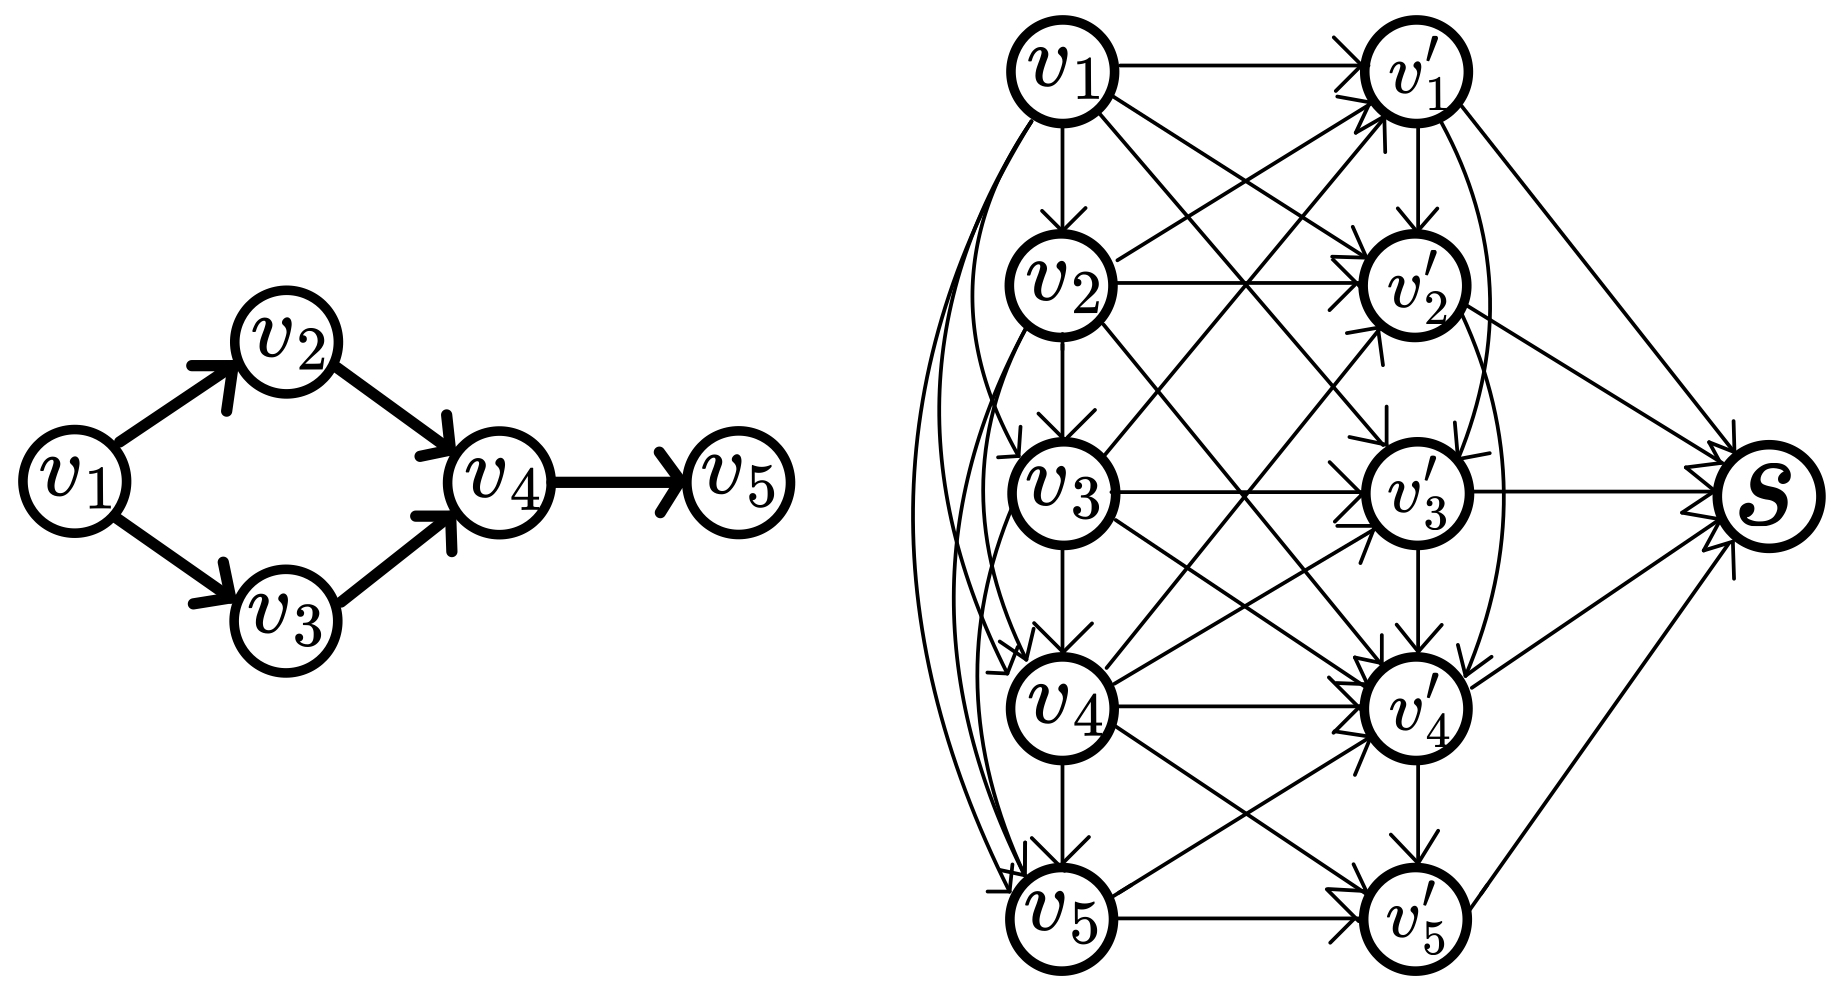
\includegraphics[width=15.0cm]{pic4.jpg}
        \caption{左の$G$から右の$G'$を構成した例.$G'$の頂点は$A = \{v_1, v_2, v_3, v_4, v_5\}, B = \{v'_1, v'_2, v'_3, v'_4, v'_5\}, \{s\}$からなる.$A$では任意の頂点対に枝があり,$B$では$G$と同じ枝の構成となっている.また$A, B$の間には$A$から$B$に向かう枝のみがあり,$B$の各頂点から$s$に向かう枝がある.}
        \label{fig:4}
    \end{figure}


    \begin{figure}[t]
        \centering
        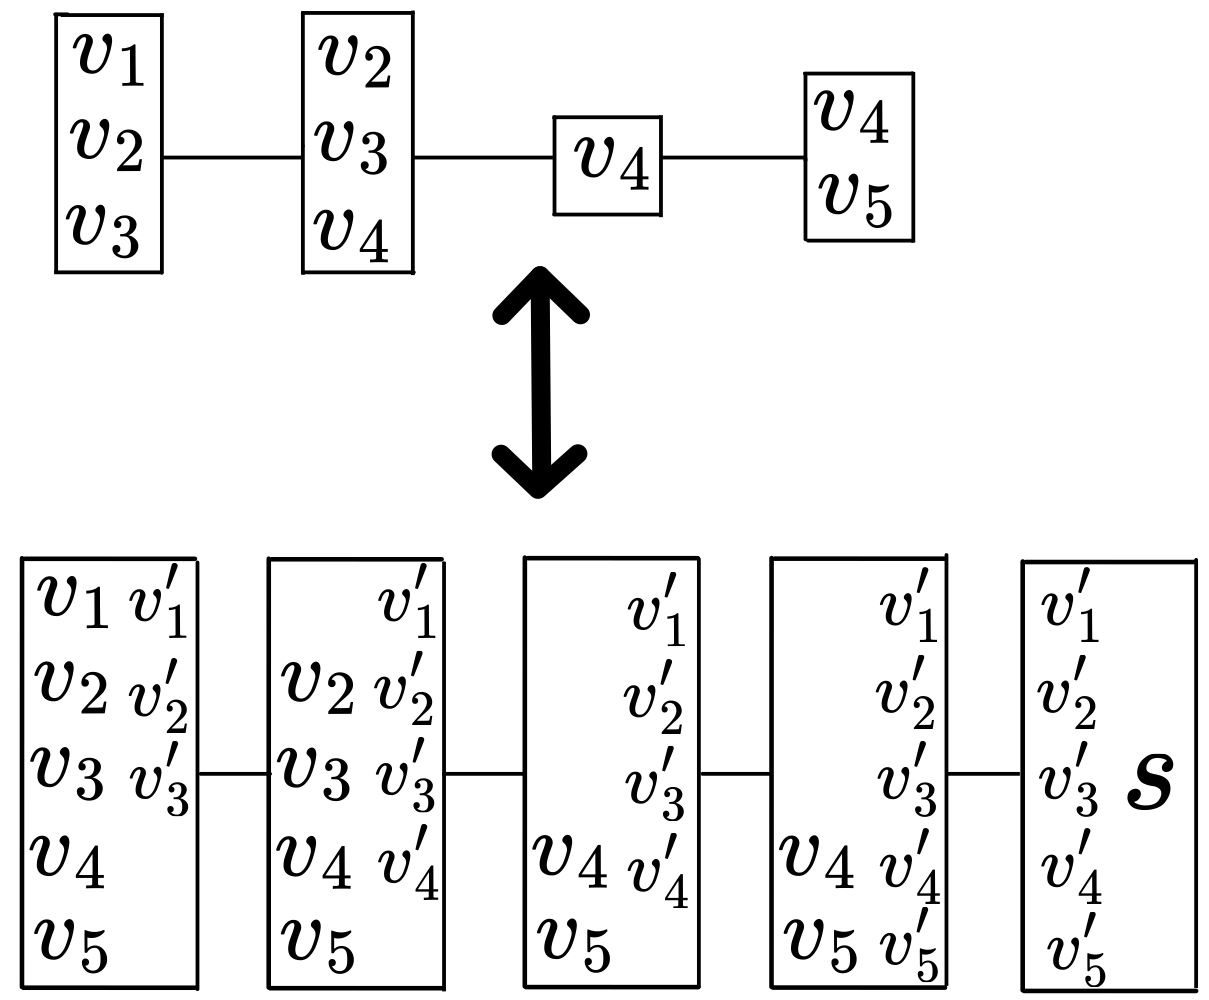
\includegraphics[width=10.0cm]{pic5.jpg}
        \caption{Figure\ref{fig:4}の$G, G'$に対するDAG-PD $(P, \beta),\ (P', \gamma)$ (それぞれ上,下)の構成例.$G$の頂点数を$n$とすると,$(P, \beta)$のwidthが$\mathsf{pw}(G)$のとき,$(P', \gamma)$のwidthは$\mathsf{pw}(G) + n$となる.}
        \label{fig:5}
    \end{figure}
}
    
    次に,widthが$\mathsf{pw}(G)$である$G$のDAG-PDを$(P, \beta)$ $(P = p_1, p_2, \dots, p_r)$とする.各$m$に対し,$G'$の頂点集合$\gamma(p_m)$を以下のように構成する.

    \vskip\baselineskip
    \begin{itemize}
        \item 各$(p_m)$に対し,$v \in \bigcup_{j = i}^{r} \beta(p_j)$ならば,$v$を$\gamma(p_m)$に加える.
        \item 各$(p_m)$に対し,$v \in \bigcup_{j = 1}^{i} \beta(p_j)$ならば,$v'$を$\gamma(p_m)$に加える.
    \end{itemize}

    さらに$\gamma(p_{r+1})$を下記のように定める.
    
    \vskip\baselineskip
    \begin{itemize}
        \item $\gamma(p_{r+1}) = B \cup \{s\}$
    \end{itemize}

    以上の操作によってできる$(P', \gamma)$ $(P' = p_1, p_2, \dots, p_{r+1})$が,$G'$のDAG-PDになっていることを示す.Figure\ref{fig:4}の$G, G'$に対するDAG-PD $(P, \beta),\ (P', \gamma)$の構成例をFigure\ref{fig:5}で示す.$\gamma$の構成法に注意すると,$\gamma(p_1)$は$A$の頂点をすべて含む.また$\gamma(p_{r+1})$は$B \cup \{s\}$を含む.よって$\sum_{m=1}^{r+1} \gamma(p_m) = V'$が成り立つため,$(P', \gamma)$はDAG-PDのルール1を満たす.また$\gamma$の構成法に注意すると,任意の$v \in V'$に対して,$v$を含む全てのバッグが$(p_1, P_2, \dots, p_r)$上で非連結になることはなく,また$\gamma(p_r)$は$B$の頂点をすべて含み,$s$は$\gamma(p_{r+1})$にのみ含まれるため,任意の$v \in V'$に対して,$v$を含む全てのバッグが$(p_1, P_2, \dots, p_r+1)$上で非連結になることはない.よって$(P', \gamma)$はDAG-PDのルール3を満たす.さらに,$(P', \gamma)$が$G'$の全ての枝に対してDAG-PDのルール2を満たすことを示す.$G'$上の各枝$e \in E'$を次の5つに場合分けして考える.なお,$v, v'$はそれぞれ$A, B$に含まれることに注意する.

    \begin{itemize}
        \item $e = (v_i, v_j)$ $(1 \leq i < j \leq n)$の場合:
        
        $A \subseteq \gamma(p_1)$より,$v_i, v_j \in \gamma(p_1)$
        \item $e = (v'_i, s)$ $(1 \leq i \leq n)$の場合:
        
        $B \cup \{s\} = \gamma(p_{r+1}), s \notin \gamma(p_r)$より,$v'_i, s \in \gamma(p_{r+1}), s \notin \gamma(p_r)$
        \item $e = (v_i, v'_i)$ $(1 \leq i \leq n)$の場合:
        
        $\gamma$の構成より,$v_i \in \beta(p_1)$ならば$v_i, v'_i \in \gamma(p_1)$.$v_i \notin \beta(p_1)$ならば,$(P, \beta)$で$v$が初めて現れたバッグを$\beta(p_m)$とすると,$v_i, v'_i \in \gamma(p_m)$であり,$v'_i$は$\gamma(p_1)$で初めて現れている.よって$v_i, v'_i \in \gamma(p_m), v'_i \notin \gamma(p_{m-1})$
        \item $e = (v_i, v'_j)$ $((v_i, v_j) \in E \in G)$の場合:
        
        $\gamma$の構成より,$v_i, v_j \in \beta(p_1)$ならば$v_i, v'_j \in \gamma(p_1)$.$v_i, v_j \notin \beta(p_1)$ならば,$(P, \beta)$において,ある$m$があり,$v_i, v_j \in \beta(p_m), v_j \neq \beta(p_{m-1})$とできる.このとき,$\gamma$の構成より$v_i, v'_j \in \gamma(p_m), v'_j \notin \gamma(p_{m-1})$
        \item $e = (v_j, v'_i)$ $((v_i, v_j) \in E \in G)$の場合:
        
        $(P, \beta)$において,$v_i$が初めて現れたバッグを$\beta(p_m)$とする.このとき$\gamma$の構成より,$v'_i$は$\gamma(p_m)$で初めて現れている.また$(P, \beta)$は$G$のDAG-PDであるから,ある$m'$があり,$v_i, v_j \in \beta(p_m'), v_j \neq \beta(p_{m'-1})$とできる.$\gamma$の構成より,$v_j \in \gamma(p_l)$ $(p_l = 1, 2, \dots, m')$がいえ,さらに$m \leq m'$に注意すると$v_j \in \gamma(p_m)$がいえる.したがって$v_j, v'_i \in \gamma(p_m), v_j \notin \gamma(p_{m-1})$
    \end{itemize}

    よって,$(P', \gamma)$はDAG-PDのルール2を満たす.以上より$(P', \gamma)$が$G'$のDAG-PDであることが示される.また,各$m = 1, 2, \dots, r$に対し,$v_i \in \beta(p_m)$ならば$v_i, v'_i \in \gamma(p_m)$であり,かつ$v_i \notin \beta(p_m)$ならば,$v_i, v'_i$のどちらか一方が$\gamma(p_m)$に含まれるため,$|\gamma(p_{r+1})| = n + 1$に注意すると,$(P', \gamma)$のwidthは$((P, \beta)$の$width)+ n$,すなわち$\mathsf{pw}(G) + n$であることがいえる.

    

    次に,$(P', \gamma)$が$G'$のDAG-PDのうち最小のwidthをもつDAG-PDであることを示す.$(P', \gamma)$よりもwidthの小さいDAG-PD $(Q, \delta)$ $(Q = (q_1, q_2, \dots, q_{r'}))$が存在すると仮定し,矛盾を導くことでこれを示す.まず,以下の手順によって$(Q, \delta)$と同じ幅をもつ$G'$のnice DAG-PDを構成する.

    \vskip\baselineskip
    \begin{enumerate}
        \item $(Q, \delta)$のバッグのうち,初めて$A$のすべての頂点が含まれたバッグを$\delta(q_i)$ $(q_i \in Q)$とする($A$の任意の2頂点間には枝があるため,このような$q_i$が存在することに注意する).ある$v' \in B$に対し,$v' \in \delta(q_j)$なる$q_j$ $(j < i)$が存在する場合,このような$q_j$を$Q$からすべて取り除く.$\delta(q_j) \subseteq \delta(q_i)$であったことに注意すると,$q_j$の削除後もwidthが同じ$G'$のDAG-PDになっており,こうしてできるDAG-PDを$(Q', \delta')$とする.
        \item $Q'$の左端に$q_0$ $(\delta'(q_0) = A)$を追加し,$(Q'', \delta'')$とする.
        \item $(Q'', \delta'')$のバッグのうち,初めて$B \cup \{s\}$のすべての頂点が含まれたバッグを$\delta''(q_k)$ $(q_k \in Q'')$とする($B$のすべての頂点から$S$に向かう枝があるため,このような$q_k$が存在することに注意する).$v \in \delta''(q_k)$なる$v \in A$が存在する場合,$Q''$から$\{q_j | j \geq k\}$をすべて取り除き,$q_{k-1}$の直後に,順に$q'_k, q'_{k+1}, q'_{k+2}$ $(\delta''(q'_k) = \delta(q_k) \backslash \{s\}, \delta''(q'_{k+1}) = B, \delta''(q'_{k+2}) = B \cup \{s\})$を追加する.この操作を行ってもDAG-PDのルールは満たされたままであり,かつwidthは操作前より大きくならないことに注意する.こうしてできるDAG-PDを$(Q''', \delta''')$とする.
        \item $(Q''', \delta''')$をwidthが同じnice DAG-PDに変換する.便宜上,このnice DAG-PDを$(Q, \delta)$ $(Q = (q_1, q_2, \dots, q_{r'})$と表記する.
    \end{enumerate}

\ifthenelse{\boolean{Draft}}{
    \begin{figure}[t]
        \centering
        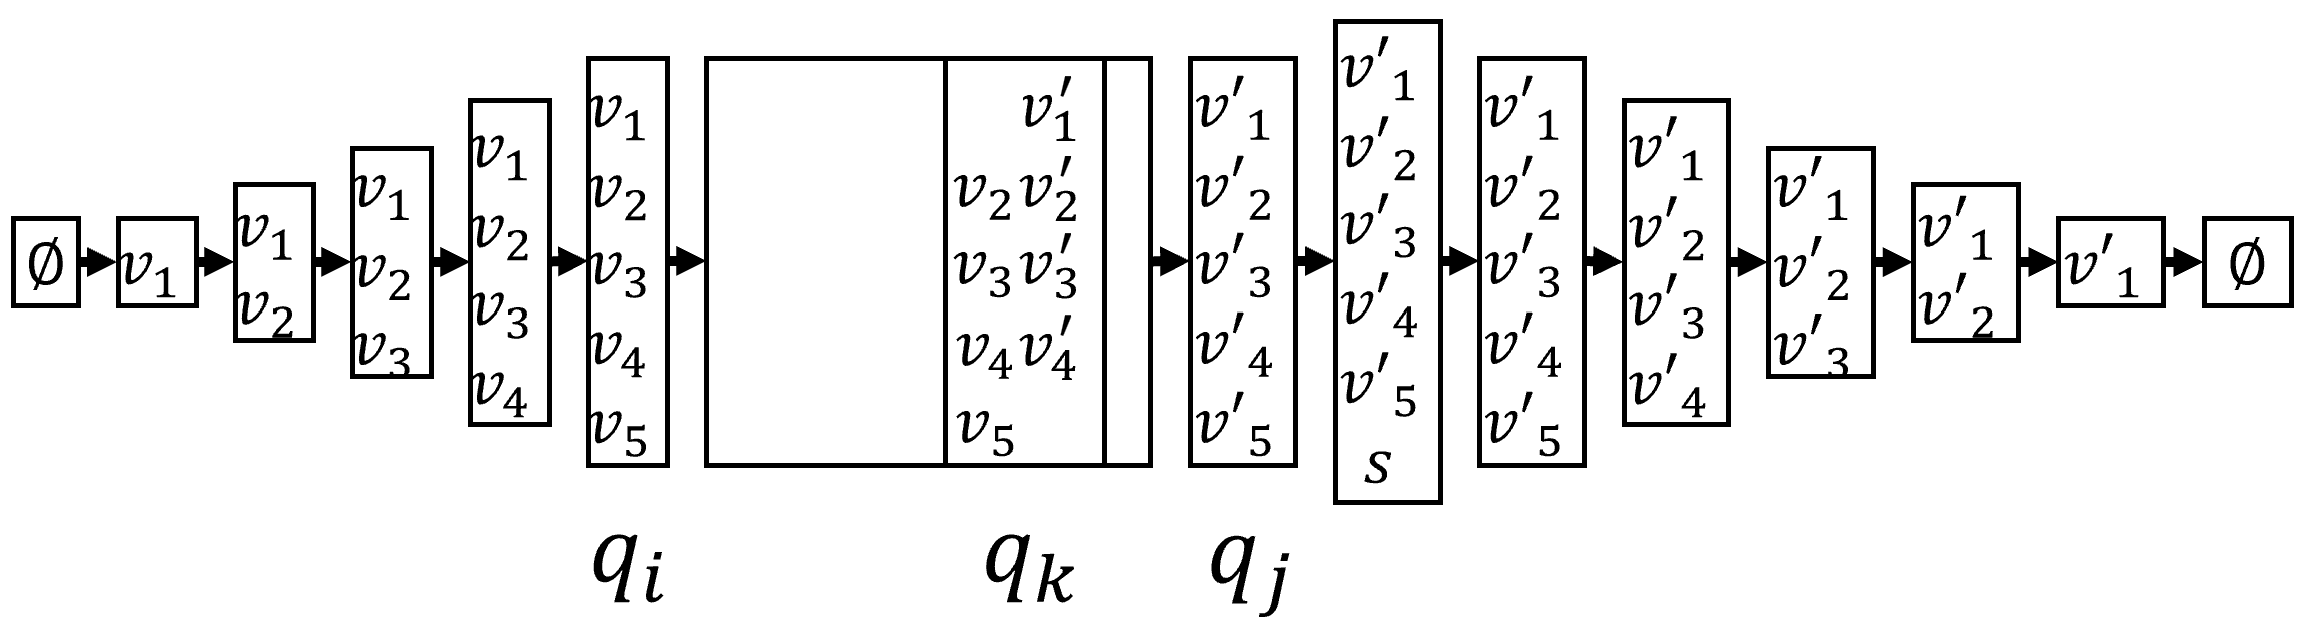
\includegraphics[width=15.0cm]{pic8.png}
        \caption{構成したnice DAG-PD $(Q, \delta)$の例.$q_i$で$A$の全ての頂点のintroduceが完了し,$q_j$で$B$の全ての頂点のintroduceが完了する.$q_i$と$q_j$の間のバッグ$q_k$では,各$i$に対して$v_i, v'_i$の少なくともどちらか一方が含まれる.}
        \label{fig:8}
    \end{figure}
}
    
    以上の操作によって構成されたnice DAG-PD $(Q, \delta)$は,はじめ$A$の頂点を順にintroduceし,ある$q_i$で$A$の全ての頂点のintroduceが終わった後,$B$の頂点のintroduceを行いつつ,$A$の頂点のfogetも行っていく.$B$のすべての頂点のintroduceが終わった後,ある$q_j$で$B$のみを含むバッグがあり,直後に$B \cup \{s\}$からなるバッグが続く.Figure\ref{fig:8}で構成後の例を示す.このとき,$\delta(q_k)$ $(q_k \in Q, i < k < j)$では,各$v_m, v'_m$ $(m = 1, 2, \dots, n)$について,$v_m, v'_m$の少なくともどちらか一方は$\delta(q_k)$に含まれる.なぜならば,$G'$には枝$(v_m, v'_m)$が存在し,$v_m, v'_m$を同時に含む$\delta(q_{i_m})$が存在すること,そして$\delta(q_i) = A, \delta(q_j) = B$に注意すると,$v_m \in \delta(q_{i_L}), v'_m \in \delta(q_{i_R})$ $(q_{i_L}, q_{i_R} \in Q, i \leq i_L \leq i_m \leq i_R \leq j)$がいえるからである.
    
    ここで各$m$ $(m = 1, 2, \dots, r')$に対し,$G$の頂点集合$\beta'(q_m)$を$\beta'(q_m) = \{v_i | \{v_i, v'_i\} \subseteq \delta(q_m) \}$と定める.このとき,$(Q, \beta')$が$G$のDAG-PDになっていることを示す.$G'$において任意の頂点対$(v, v')$ $(v \in A, v' \in B)$が隣接していることに注意すると,$(Q, \delta)$では$(v, v')$を同時に含むようなバッグが少なくとも1つ存在する.よって$\sum_{m=1}^{r'}\beta'(q_r') = V$が成り立つため,$(Q, \beta')$はDAG-PDのルール1を満たす.また$G'$のうち$B$によって誘導される部分グラフを$G'_B$とすると,$E(G'_B) = E(G)$であるため,$B$の頂点でintroduceされる順序は,$G'$の強連結成分に対するトポロジカル順序になる.したがって$(Q, \beta')$も$G'$の強連結成分がトポロジカル順序でintroduceされていくため,$(Q, \beta')$はDAG-PDのルール2を満たす.さらに,$(Q, \delta)$は$G'$のDAG-PDであるから,$(Q, \delta)$で$A$の頂点が一度forgetされた後,再びintroduceされることはない.よって$(Q, \delta)$で${v, v'}$を含むバッグが非連結になることはないため,$(Q, \beta')$でも$v$を含むバッグが非連結になることはない.したがってDAG-PDのルール3を満たす.

    以上より,$(Q, \beta')$は$G$のDAG-PDになっている.このとき,$(Q, \beta')$の各バッグは,$(Q, \delta)$の各バッグが$(v_i, v'_i)$を同時に含む場合のみ$v_i$を含んでいること,そして各$\delta(q_m)$には$v_i, v'_i$の少なくともどちらか一方が含まれることに注意すると,$(Q, \delta)$のwidth $k$に対し,$(Q, \beta')$のwidth $w_b$は高々$k - n$である.ここで仮定より$k < \mathsf{pw}(G) + n$であるため$w_b < \mathsf{pw}(G)$とできるが,これは$\mathsf{pw}(G)$が$G$のDAG-pathwidthであることと矛盾する.したがって仮定が誤りであり,$(P', \gamma)$が$G'$のDAG-PDのうち最小のwidthをもつDAG-PDであることが示される.
    
    以上より,$\mathsf{pw}(G') = \mathsf{pw}(G) + n$が導かれる.$G'$がsinkをただ1つもつこととLemma~\ref{sink}とより$\mathsf{tw}(G') = \mathsf{pw}(G')$がいえるため,$\mathsf{pw}(G') = \mathsf{tw}(G') = \mathsf{pw}(G) + n$が導かれる.
    
\end{proof}








\section{Theorem~\ref{r-NP困難}の証明}

Theorem~\ref{r-NP困難}を証明するため,次で定義されるco-DAG-pathwidthの計算がNP困難であることを示す.

\begin{definition*}
     $G=(V, E)$とする.$G$のco-DAG Path Decomposition (co-DAG-PD)とは,以下の3つの条件をみたすようなVの各部分集合$ X_i (i = 1, 2,  \ldots, s)$の列 $X=(X_1, X_2,  \ldots, X_s)$ である.

    \begin{enumerate}
        \item $ X_1 \cup X_2 \cup \dots \cup X_s = V $ 
        \item 任意の有向枝 $ (u, v) \in E $ について,以下のいずれかが成り立つ.
        \begin{itemize}
            \item $u, v \in X_1$
        \item ある $i$ $(i \geq 2)$ があり,$u, v \in X_i$, $u \notin X_{i-1}$が成り立つ.
        \end{itemize}
        \item 任意の$ i, j, k\ (1 \leq i \leq j \leq k \leq s)$ について, $X_i \cap X_k \subseteq X_j$ が成り立つ.すなわち,各頂点$v$について,$v$は$X$上で非空な部分道を誘導する.
    \end{enumerate}
    あるco-DAG-PD $P = (X_1, X_2,   \ldots, X_s)$のwidthを$\max_{1 \leq i \leq s} {X_i}$と定義する.このとき,有向グラフ$G$のco-DAG-pathwidthとは,$G$に対する全てのco-DAG-PDのうち,widthが最小であるco-DAG-PDのwidthである.
    
\end{definition*}
 
以降では,$G$のco-DAG-pathwidthを$\mathsf{cpw}(G)$と表す.





\begin{lemma}\label{co-DAG-PD}
    有向グラフ$G$,整数$k$が与えられたとき,$\mathsf{cpw}(G) \leq k$が成り立つかを判定する問題はNP完全である.
\end{lemma}

\begin{proof}
    $G$のあるco-DAG-PDが与えられたとき,そのwidthが$k$以下かどうかを判定することは明らかに多項式時間で行えるため,この問題はNPに属する.また,$G$の全ての枝の向きを逆にした有向グラフを$G'$とする.$G$に対してwidthが$\mathsf{pw}(G)$であるDAG-PD $P$が与えられたとき,$G'$に対して最小のwidthをもつco-DAG-PD $P'$は,DAG-PDとco-DAG-PD定義より$P$と等しい.したがって$P'$のwidthは$\mathsf{pw}(G)$であるため,$\mathsf{cpw}(G')= \mathsf{pw}(G)$が成り立つ.以上よりLemma~\ref{co-DAG-PD}が示される.
\end{proof}





また,次のLemmaを示す.

\begin{lemma}\label{r-sink}
    $G =(V, E)$が$sink$をただ1つしか持たないならば,$\mathsf{ctw}(G) = \mathsf{cpw}(G)$が成り立つ.
\end{lemma}

\begin{proof}
    co-DAG-PD, co-DAG-TDの定義より,widthが$\mathsf{cpw}(G)$である$G$のco-DAG-PDは$G$のco-DAG-TDでもある.よって$\mathsf{ctw}(G) \leq \mathsf{cpw}(G)$が成り立つ.一方,widthが$\mathsf{ctw}(G)$である$G$のnice co-DAG-TDを$(T, \gamma)$とし,$G$のただ一つの強連結成分であるsinkを$A \subseteq V$とする.このときnice co-DAG-TDの定義より,ある根$r$とその子$r_c$があり,$\gamma(r) = \varnothing, \gamma(r_c) = A$が成り立つ.このとき$T$はただ一つの根$r$をもつことがいえる.なぜならば,もし$T$が$r$以外の根$r'$ $(\gamma(r') = \varnothing)$をもつと仮定すると,$r'$の子はバッグに$A$を含まないため,$G$に$A$以外のsinkが存在することになり,矛盾するからである.したがって$T$はunionのノードを持たず,任意の$t \in T$は入次数と出次数が高々1である.したがってco-DAG-PDとco-DAG-TDの定義より,$(T, \gamma)$は$G$のDAG-PDでもある.これより$\mathsf{cpw}(G) \leq \mathsf{ctw}(G)$がいえる.以上より,$\mathsf{ctw}(G) = \mathsf{cpw}(G)$が示される.
\end{proof}





最後にTheorem~\ref{r-NP困難}を示す.

\begin{proof}
    ある有向グラフ$G = (V, E)$が与えられたとき,定義\ref{NP困難}の証明と同様の手順で$|V'| = 2|V| + 1, |E'| = \frac{1}{2}(|V|^2 + 3|V|) + 2|E|$である有向グラフ$G' = (V', E')$ を構成する.また$G'$の頂点集合$A, B$を同様に$A = \{v_i | i =1, 2, \dots, n\}, B = \{v'_i | i =1, 2, \dots, n\}$と定める.このとき$V' = A \cup B \cup \{s\}$とできる.$G'$は$G$のサイズの多項式時間で構成できる.
    
    次に,widthが$\mathsf{cpw}(G)$である$G$のco-DAG-PDを$(P, \beta)$ $(P = p_1, p_2, \dots, p_r)$とする.各$m$に対し,$G'$の頂点集合$\gamma(p_m)$を以下のように構成する.

    \vskip\baselineskip
    \begin{itemize}
        \item 各$(p_m)$に対し,$v \in \bigcup_{j = i}^{r} \beta(p_j)$ならば,$v'$を$\gamma(p_m)$に加える.
        \item 各$(p_m)$に対し,$v \in \bigcup_{j = 1}^{i} \beta(p_j)$ならば,$v$を$\gamma(p_m)$に加える.
    \end{itemize}

    さらに$\gamma(p_0) = \gamma(p_1) \cup \{s\}$ $((p_0, p_1) \in E[T])$と定める.

    以上の操作によってできる$(P', \gamma)$ $(P' = (p_0, p_1, p_2, \dots, p_r))$が$G'$のco-DAG-PDになっていることを示す.
    % Figure★★\ref{fig:4_2}の$G, G'$に対するco-DAG-PD $(P, \beta),\ (P', \gamma)$の構成例をFigure★★\ref{fig:5_2}で示す.
    $\gamma$の構成法に注意すると,$A \subseteq \gamma(p_r), B \subseteq \gamma(p_1)$がいえ,さらに$r \in \gamma(p_0)$であることから,$\sum_{m=0}^{r} \gamma(p_m) = V'$が成り立つ.よって$(P', \gamma)$はco-DAG-PDのルール1を満たす.また$\gamma$の構成法に注意すると,任意の$v \in V' \backslash \{r\}$に対して,$v$を含む全てのバッグが$(p_1, p_2, \dots, p_r)$上で非連結になることはなく,また$B \cup \{r\} \subseteq \gamma(p_0)$より,任意の$v \in V'$に対して,$v$を含む全てのバッグが$(p_0, p_1, p_2, \dots, p_r)$上で非連結になることはない.よって$(P', \gamma)$はco-DAG-PDのルール3を満たす.さらに定義\ref{NP困難}の証明と同様の議論により,$(P', \gamma)$がco-DAG-PDのルール2を満たすことがいえる.以上より$(P', \gamma)$は$G'$のco-DAG-PDである.このとき$(P', \gamma)$の幅は$\mathsf{cpw}(G)+n$である.

    さらに\ref{NP困難}の証明と全く同様の議論により,$(P', \gamma)$が$G'$に対してwidthが最小のco-DAG-PDであることがいえる.ここで$G'$はsinkを一つしか持たないことに注意すると,Lemma~\ref{r-sink}より$\mathsf{ctw}(G') = \mathsf{cpw}(G')$がいえ,$\mathsf{ctw}(G) = \mathsf{cpw}(G) + n$が成り立つ.以上より定義\ref{r-NP困難}が示される.
\end{proof}










\section{Lemma~\ref{dids2}の証明}



\begin{proof}
    $i=l$のとき,定義\ref{def_ds2}より$\mathsf{DS}$はmDiDSのサイズを出力する.したがって各$i \in T$に対し,$\mathsf{DS}(i, A_i, B_i)$が$\mathsf{DS}$の定義\ref{def_ds}を満たすことを示せば十分.これを$i$に関する数学的帰納法で示す.
    まず$i$が$T$の根のとき$\beta(i) = \varnothing$であり,First Stepより明らかに定義\ref{def_ds2}を満たす.
    次にある$i$での定義\ref{def_ds2}の成立を仮定する.以下で$i$の子$i'$がintroduceかforgetかunionかで場合分けを行う.
    \begin{itemize}
        \item $i'$が$v \in V$をintroduceする場合 \\
        $i'$はただ一つの親$i$をもつ.$v \in A_{i'}$の場合,co-DAG-TDのルール2より$v$の後続頂点は$i'$の時点で全てintroduceされており,$v$は$\mathsf{suc}(v)$を支配する.またco-DAG-TDのルール2より$v$は$i'$の時点でどの頂点からも支配されていない.仮定より$D = \mathsf{DS}(i, A_{i'}, B_{i'})[1]$が支配されれば$G_i$のmDiDSのサイズは$\mathsf{DS}(i, A_{i'}, B_{i'})[0]$であるから,$D \backslash \mathsf{suc}(v)$が支配されれば$G_{i'}$のmDiDSのサイズは$\mathsf{DS}(i, A_{i'}, B_{i'})[0] + |v|$となる.したがって$i'$でも定義\ref{def_ds2}を満たす.

        $v \in B_{i'}$の場合,$v$は支配集合に含まれないので$i'$以降にintroduceされる頂点によって支配される必要がある.仮定より$D = \mathsf{DS}(i, A_{i'}, B_{i'})[1]$が支配されれば$G_i$のmDiDSのサイズは$\mathsf{DS}(i, A_{i'}, B_{i'})[0]$であるから,$D \cup \{v\}$が支配されれば$G_{i'}$のmDiDSのサイズは$\mathsf{DS}(i, A_{i'}, B_{i'})[0]$となる.したがって$i'$でも定義\ref{def_ds2}を満たす.
        
        \item $i'$が$v \in V$をforgetする場合 \\
        $i'$はただ一つの親$i$をもつ.$v \in \mathsf{DS}(i, A_{i'}, B_{i'} \cup \{v\})[1]$の場合,$v$を支配する頂点は$A_{i'}$に存在しないため,$i$の時点で$v$自身が支配集合に含まれている必要がある.逆にこのとき,仮定より$\mathsf{DS}(i, A_{i'} \cup \{v\}, B_{i'})[1]$が支配されれば$G_i$のmDiDSのサイズは$\mathsf{DS}(i, A_{i'} \cup \{v\}, B_{i'})[0]$であるため,$i'$でも定義\ref{def_ds2}を満たす.

        $v \notin \mathsf{DS}(i, A_{i'}, B_{i'} \cup \{v\})[1]$の場合,$v$を支配する頂点が$A_{i'}$に少なくとも1つ存在する.したがって$v$は$i$の時点で$A_{i'}, B_{i'}$のいずれに含まれていてもよく,またmDiDSのサイズが小さくなるのは$v$が$B_{i'}$に含まれている場合である.仮定より$\mathsf{DS}(i, A_{i'}, B_{i'} \cup \{v\})[1]$が支配されれば$G_i$のmDiDSのサイズは$\mathsf{DS}(i, A_{i'}, B_{i'} \cup \{v\})[0]$であるため,$i'$でも定義\ref{def_ds2}を満たす.

        \item $i'$が二つの親$i, \overline{i}$をもつunionであるとき \\
        $\overline{i}$においても定義\ref{def_ds2}が成立していると仮定する.また$D_i = \mathsf{DS}(i, A_i, B_i)[1], D_{\overline{i}} = \mathsf{DS}(\overline{i}, A_{\overline{i}}, B_{\overline{i}})[1]$とする.以下では$A_{i'} = A_{i} = A_{\overline{i}}, B_{i'} = B_{i} = B_{\overline{i}}$であることに注意する.$D_i = D_{\overline{i}}$の場合,仮定より$D_i$が支配されれば$S_i$は$G_i$のmDiDSであり,かつ$D_i$が支配されれば$S_{\overline{i}}$は$G_{\overline{i}}$のmDiDSである.このとき$S_{i} \cap S_{\overline{i}} = A_{i'}$が成り立つ.なぜならば定義\ref{def_ds2}より$B_{i} \cap S_i = \varnothing, B_{\overline{i}} \cap S_{\overline{i}} = \varnothing$であり,co-DAG-TDのルール3より任意の$s \in S_{i} \cap S_{\overline{i}}$を含むバッグは$T$上で$i', i, \overline{i}$を含む連結な反有向木を形成しているからである.したがって$V[G_{i'}] = V[G_i] \cup V[G_{\overline{i}}]$に注意すると,$D_i$が支配されれば$S_i \cup S_{\overline{i}}$は明らかに$G_{i'}$のmDiDSである.このときmDiDSのサイズは$\mathsf{DS}(i, A_{i'}, B_{i'})[0] + \mathsf{DS}(\overline{i}, A_{i'}, B_{i'})[0] - |A_{i'}|$であるため$i'$でも定義\ref{def_ds2}を満たす.

        $D_i \neq D_{\overline{i}}$の場合,$D_{\overline{i}} \backslash D_i \neq \varnothing$としても一般性を失わない.このときある頂点$w \in D_{\overline{i}} \backslash D_i$が存在する.定義\ref{def_ds2}より$w$は$B_{\overline{i}} = B_{i} = B_{i'}$に含まれ,かつ$w$はある頂点$w' \in S_i\subseteq V[G_i]$によって支配されており,$S_{\overline{i}}$には$w$を支配する頂点が存在しない.ここで$V[G_{i'}] = V[G_i] \cup V[G_{\overline{i}}]$であるから,$S_{i'} = S_i \cup S_{\overline{i}}$とすることで$S_{i'}$には$w$を支配する$w'$が含まれる.したがって仮定に注意して$D_i \cap D_{\overline{i}}$が支配されれば$S_i \cup S_{\overline{i}}$は明らかに$G_{i'}$のmDiDSである.上記と同様の議論により$|S_i \cup S_{\overline{i}}| = \mathsf{DS}(i, A_{i'}, B_{i'})[0] + \mathsf{DS}(\overline{i}, A_{i'}, B_{i'})[0] - |A_{i'}|$であるため,$i'$においても定義\ref{def_ds2}を満たす.
        
    \end{itemize}
    以上より,$i'$でも定義\ref{def_ds2}が成立.数学的帰納法によりLemma~\ref{dids2}が証明された.
\end{proof}






% この手引で述べた教室所定の形式に適合した論文を\LaTeX で作成するために,スタ
% イルファイル\|kuisthesis|が用意されている.以下,\|kuisthesis|を使う
% ための準備と,その使用法について解説する.

% なお,この手引自体も\|kuisthesis|を用いて作成したものであるので,必要に
% 応じてスタイルファイルとともに配布されるソースファイル\|guide.tex|を参照
% するとよい.

% また,論文作成の際に使用する\LaTeX コマンドのほとんどは標準的なものであるの
% で,基本的な使用法やここで解説していないものについては
% \begin{quote}%{
% Lamport, L.: {\em A Document Preparation System {\LaTeX} User's Guide \&
% Reference Manual\/}, Addison Wesley, Reading, Massachusetts (1986).
% (Cooke, E., et al.訳:文書処理システム{\LaTeX}, アスキー出版局(1990)).
% \end{quote}%}
% などを適宜参照されたい.

% \section{準備}\label{app-prelim}
% \subsection{スタイルファイルなどの取得}\label{appsub-kit}
% スタイルファイル\|kuisthesis|や,その他の関連するファイルからなるキット
% は
% \begin{itemize}\item[]\small%{
% \|ftp://ftp.kuis.kyoto-u.ac.jp/ku/kuis-thesis/kuisthesis.tar.gz|
% \end{itemize}%}
% に\|tar|${}+{}$\|gzip|の形式で収められている.

% このキットには,以下のファイルが格納されている.
% \begin{itemize}%{
% \item
% \|kuisthesis.sty|\,:
% スタイルファイル
% \item
% \|kuisthesis.cls|\,:
% {\LATEXe}用スタイルファイル
% \item
% \|kuissort.bst  |\,:
% jBib\TeX スタイル(著者名順)
% \item
% \|kuisunsrt.bst |\,:
% jBib\TeX スタイル(出現順)
% \item
% \|guide.tex     |\,:
% この手引のソースファイル
% \item
% \|guide.bib     |\,:
% この手引の文献リスト
% \item
% \|eguide.tex    |\,:
% 英文の手引のソースファイル
% \item
% \|guide.bib     |\,:
% 英文の手引の文献リスト
% \end{itemize}%}
% 
% \subsection[{\protect\LaTeX}の実行環境]{{\protect\LATex}の実行環境}
% \label{appsub-env}
% スタイルファイルはNTTの斉藤康己氏による j{\TeX}(いわゆるNTT版)と,アスキー
% 社による日本語 {\TeX}(いわゆるアスキー版)のどちらにも対応しているので,著者
% の {\LaTeX} 環境に関わらず同じスタイルファイルを使用できる.

% NTT版およびアスキー版の各々について,以下のバージョンでの動作確認を行なって
% いる.
% \begin{ITEMIZE}%{
% \item
% NTT版${}={}${j\TeX} 1.52${}+{}${\LaTeX} 2.09
% \item 
% アスキー版${}={}${\TeX} 2.99-j1.7${}+{}${\LaTeX} 2.09
% \end{ITEMIZE}%}
% これ以前の版についても動作すると期待できるが,できれば新しい版を使うこと.ま
% た{\LATEXe}に関しては,以下のバージョンでの動作確認を行なっている.
% \begin{ITEMIZE}%{
% \item
% NTT版${}={}${j\TeX} 1.6${}+{}$%
% 	{\LATEXe} 1994/12/01 patch level 3
% \item 
% アスキー版${}={}${p\TeX} 3.1415 p2.1.4${}+{}$%
% 	{p\LATEXe} 1995/09/01
% \end{ITEMIZE}%}
% いずれについても,ネイティブ・モードと{\LaTeX} 2.09 互換モードのどちらでも使
% 用することができる.

% 論文を英文で書く場合にも,和文の内容梗概が必要であるので,必ず日本語対応の
% \LaTeX を使用しなければならない.
% 
% \section{ソースファイルの構成}\label{app-structure}
% ソースファイルは以下の形式で作る.
% \begin{itemize}\item[]%{
% \|\documentclass{kuisthesis}|または\\
% \|\documentclass[master]{kuisthesis}|または\\
% \|\documentclass[master,english]{kuisthesis}|\\
% \null\qquad 必要ならば他のオプションやスタイルファイルを指定する.\\
% 必要ならばユーザのマクロ定義などをここに書く.\\
% \|\jtitle{|\<題目(和文)\>\|}|\\
% \|\etitle{|\<題目(英文)\>\|}|\\
% \|\jauthor{|\<著者名(和文)\>\|}|\\
% \|\eauthor{|\<著者名(英文)\>\|}|\\
% \|\supervisor{|\<指導教官名\>\|}|\\
% \|\date{|\<提出年月日\>\|}|\\
% \|\department{|\<専攻名\>\|}|\\
% \|\begin{document}|\\
% \|\maketitle|\hfill\rlap{\hskip-.5\linewidth{\tt\%}とびらの出力}\\
% \|\begin{jabstract}|\\
% \null\qquad\<内容梗概(和文)\>\\
% \|\end{jabstract}|\\
% \|\begin{eabstract}|\\
% \null\qquad\<内容梗概(英文)\>\\
% \|\end{eabstract}|\\
% \|\tableofcontents|\hfill\rlap{\hskip-.5\linewidth{\tt\%}目次の出力}\\
% \|\section{|\<第1章の表題\>\|}|\\
% \null\qquad\hbox to3em{\dotfill}\\
% \null\qquad\<本文\>\\
% \null\qquad\hbox to3em{\dotfill}\\
% \|\acknowledgments|\\
% \null\qquad\<謝辞\>\\
% \|\bibliographystyle{kuisunsrt}|\quad または\\
% \|\bibliographystyle{kuissort}|\\
% \|\bibliography{|\<文献データベース\>\|}|\\
% 付録があれば \|\appendix|/\|\Appendix| に続いてここに記す.\\
% \|\end{document}|
% \end{itemize}%}
% 以下,それぞれの要素について説明する.
% 
% \subsection{印字の形式}\label{appsub-format}
% 論文の各ページは,幅(\|\textwidth|) 14.2\,cm, 高さ(\|\textheight|) 
% 22.2\,cmの領域に印刷される\footnote{NTT版では和文の場合,幅 
% ({\tt\string\textwidth})が 13.6\,cmとなる}.この幅は和文の場合には35文字分に
% 相当し,高さは和文/英文とも32行分に相当するので,\ref{subsec-format}節に
% 示した基準に合致している.

% 和文/英文とも\|\normalsize|のフォントは12\,ptであり,これも
% \ref{subsec-format}節の基準を満たしている.
% 
% \subsection{オプション・スタイル}\label{appsub-option}
% \|\documentclass|の標準オプションとして,以下の3つのものが用意されている.
% \begin{itemize}%{
% \item
% \|master|\\
% 修士論文用.指定がなければ特別研究報告用となる.なお両者の違いは,とびらに印
% 字される論文種別と所属のみであり,ページ数のチェックなどは一切行なわない.
% \item
% \|english|\\
% 英文用.指定がなければ和文用となる.特別研究報告書は必ず和文であるので, 
% \|master|を指定せずに\|english|を指定するのは誤りであるが,特にチェックはし
% ない.
% \item
% \|withinsec|\\
% 図表番号や数式番号を,``\<章番号\>.\<章内番号\>''の形式とする.指定がなけれ
% ば,論文全体で通し番号となる.
% \end{itemize}%}

% この他に,\|epsf|など補助的なスタイルファイルを指定してもよい.ただしスタイ
% ルファイルによっては,論文スタイルと矛盾するようなものもあるので,スタイルファ
% イルの性格をよく理解して使用すること.たとえば,\|a4|はページの高さである
% \|\textheight|を変更するので,使用してはならない.
% 
% \subsection{題目などの記述}\label{appsub-title}
% 論文の題目,著者名,および指導教官名を前に示した所定のコマンドで指定した後,
% \|\maketitle|を実行すると,とびらが生成される.

% とびらには,以下の項目がそれぞれセンタリングされて,順に印字される.
% \begin{description}%{
% \item[論文種別]
% 「特別研究報告」,「修士論文」,または``Master Thesis''のいずれかが,
% \|\documentclass|のオプションにしたがって,\|\Large\bf|で印字される.

% \item[題目]
% 和文の場合には\|\jtitle|で,英文の場合には\|\etitle|で指定した題目が,それぞ
% れ\|\LARGE\bf|で印字される.一行に収まらない場合には自動的に改行されるが,適
% 切な箇所に\|\\|を挿入して陽に改行を指示するほうがよい.

% \|\jtitle|や\|\etitle|で指定した題目は,とびらだけではなく内容梗概や目次にも
% 印字される.したがって和文/英文に関わらず,\|\jtitle|と\|\etitle|の双方を指
% 定しなければならない.また,とびらと内容梗概/目次では,題目の改行を違う位置
% で行ないたいこともあるだろう.その場合
% \begin{quote}%{
% \|\jtitle[|\<内容梗概/目次用\>\|]{|\<とびら用\>\|}|\\
% \|\etitle[|\<内容梗概/目次用\>\|]{|\<とびら用\>\|}|
% \end{quote}%}
% のように,オプション引数で内容梗概や目次のページに印字する題目を別途指定する
% ことができる.例えばこの手引では
% \begin{quote}\begin{verbatim}
% \jtitle[特別研究報告書・修士論文執筆の手引]%
%        {特別研究報告書・修士論文\\執筆の手引}
% \end{verbatim}\end{quote}
% として,とびらでは2行,内容梗概や目次では1行になるようにしている.

% \item[指導教官名]
% \|\supervisor|で指定した指導教官の氏名と職名を\|\large|で印字する.氏名/職
% 名は,本文に用いる言語に応じて適切に指定すること.

% \item[所属学科/専攻]
% \|\documentclass|のオプションと入学年次に応じて,以下のいずれかが\|\large|で
% 印字される.
% \begin{itemize}%{
% \item 特別研究報告書(平成6年以前入学)\\
% 京都大学工学部情報工学科
% \item 特別研究報告書(平成7年以降入学)\\
% 京都大学工学部情報学科
% \item 修士論文(和文)\\
% 京都大学大学院工学研究科情報工学専攻
% \item 修士論文(英文)\\
% Department of Information Science,
% Graduate School of Engineering\\
% Kyoto University
% \end{itemize}%}
% なお学部4回生の入学年次は,\LaTeX を実行した日をもとに,その4年前であると仮
% 定して算出している.何らかの理由でこの仮定が成り立たない場合には
% \begin{quote}\begin{verbatim}
% \setcounter{entranceyear}{1993}
% \end{verbatim}\end{quote}
% のように,カウンタ\|entranceyear|に入学年次を西暦でセットすること.

% \item[著者名]
% 和文の場合には\|\jauthor|で,英文の場合には\|\eauthor|で指定した著者名が,そ
% れぞれ\|\Large|で印字される.題目と同様,\|\jauthor|と\|\eauthor|は内容梗概
% のページにも印字されるので,和文/英文に関わらず双方を指定すること.

% \item[提出年月日]
% \|\date|で指定した日付が\|\large|で印字される.日付は,本文に用いる言語に応
% じて適切に指定すること.

% \item[専攻名]
% 修士論文の場合,\|\department|で指定した専攻名が印字される.例えば,
% 和文の場合
% \begin{quote}\begin{verbatim}
% \department{社会情報学}
% \end{verbatim}\end{quote}
% 英文の場合
% \begin{quote}\begin{verbatim}
% \department{Social Informatics}
% \end{verbatim}\end{quote}
% のように指定する.
% \end{description}
% とびらのページにはページ番号が印字されないが,出力の便宜を図るためにdviファ
% イルにはページ番号1000が付与されている.
% 
% \subsection{内容梗概}\label{appsub-abstract}
% 和文の内容梗概を\|jabstract|環境の中に,また英文の内容梗概を\|eabstract|環境
% の中に,それぞれ記述する.それぞれの内容梗概の前には,前述の\|\jtitle|や
% \|\etitle|で指定した題目と,\|\jauthor|や\|\eauthor|で指定した著者名が出
% 力される.

% それぞれの内容梗概は,記述した順序で出力される.したがって,本文が和文の場合
% には和文\,$\to$\,英文の順で,また本文が英文の場合には英文\,$\to$\,和文の順で
% 記述するのが適当である.

% 内容梗概のページ番号は,ページの右肩に小文字のローマ数字で印字される.また出
% 力の便宜を図るために,dviファイルの各ページには印字されるページ番号に1000を
% 加えたものが付与される.
% 
% \subsection{目次}\label{appsub-toc}
% コマンド\|\tableofcontents|により,目次が生成される.目次の最上部には,前述
% の\|\jtitle|\slash\|\etitle|で指定した題目が印字される.

% デフォルトでは,\|\section|, \|\subsection|, および\|\subsubsection|の見出し
% とそれらのページ番号が目次に含まれる.これを変更し,たとえば\|\section|と
% \|\subsection|のみの目次にしたい時には
% \begin{quote}\begin{verbatim}
% \setcounter{tocdepth}{2}
% \end{verbatim}\end{quote}
% により,カウンタ\|tocdepth|の値を目次に含まれる最下位の章・節レベル
% に設定すればよい.なお\|\section|のレベルは1である.

% この他,「謝辞」と「参考文献」も番号のない\|\section|として目次に含まれる.
% さらに(もしあれば)「付録」と,付録の中の\|\section|と\|\subsection|も含ま
% れる.

% 目次のページにはページ番号を印字しないが,dviファイルには内容梗概に続く1000
% 番台のページ番号が付与される.
% 
% \subsection{章・節}\label{appsub-sectioning}
% 章や節の見出しには,通常どおり\|\section|, \|\subsection|, \|\subsubsection|
% などを使用する.

% \|\section|の見出しは2行を占め,\|\Large\bf|で印字される.修士論文の
% 場合は改頁が行なわれる.
% \|\subsection|の見出しは1行の空白を置いた後に\|\large\bf|で印字され,引
% き続く文章との間には余分な空白は挿入されない.\|\subsubsection|は
% 上部に空白が挿入されず,\|\normalsize\bf|で印字される.

% デフォルトでは,上記の3つのコマンドによる章・節の見出しに,章番号や節番号が
% 付けられ,下位の章・節コマンドである\|\paragraph|, \|\subparagraph|による見
% 出しには番号が付けられない.また,これらの下位コマンドによる見出しと引き続く
% 文章の間では改行が行なわれない.
% 
% \subsection{図表}\label{appsub-figure}
% 図や表は,通常と同じく\|figure|や\|table|環境の中に記述する.図表の番号は,
% デフォルトでは論文全体の通し番号であるが,前述の\|\documentclass|のオプショ
% ン\|withinsec|を使用すると,章の中で番号づけが行なわれ,章番号と組み合わされ
% る.

% 紙面の節約のために,図表を横に並べて置きたいことがある.このような場合のため
% に,\|subfigure|と\|subtable|という2つの環境が用意されている.たとえば図
% \ref{fig-example}と表\ref{tab-example}は
% \begin{quote}%{
% \|\begin{figure}|\\
% \|\begin{subfigure}{0.6\textwidth}|\\
% \null\qquad\<図\ref{fig-example}の中身\>\\
% \|\caption{図の例}|\\
% \|\end{subfigure}|\\
% \|\begin{subtable}{0.4\textwidth}|\\
% \|\caption{表の例}|\\
% \null\qquad\<表\ref{tab-example}の中身\>\\
% \|\end{subtable}|\\
% \|\end{figure}|
% \end{quote}%}
% により生成したものである.なおこの例では\|figure|環境の中に\|subfigure|と
% \|subtable|を入れているが,\|table|環境の中に入れてもよい.

% \|subfigure|と\|subtable|の仕様は,\|minipage|と同様であり
% \begin{itemize}\item[]%{
% \|\begin{subfigure}[|\<位置\>\|]{|\<横幅\>\|}|\quad\<中身\>\quad
% \|\end{subfigure}|\\
% \|\begin{subtable}[|\<位置\>\|]{|\<横幅\>\|}|\quad\<中身\>\quad
% \|\end{subtable}|
% \end{itemize}%}
% である.また環境中の\|\caption|コマンドにより,それぞれの見出しが生成される.

% 横に並べる\|subfigure|\slash\|subtable|の横幅の合計が,
% \|\textwidth|に一致するようにするのが望ましい\footnote{各々の間に
% {\tt\string\hspace\char`\{\string\fill\char`\}}を挿入するなどして,間隔を置く
% こともできる.}.
% 
% \begin{figure}%{
% \begin{subfigure}{.6\textwidth}
% \centerline{\fbox{\vbox to.1\textheight{\vss
% 	\hbox to.8\textwidth{\hss This is a figure\hss}\vss}}}
% \caption{図の例}\label{fig-example}
% \end{subfigure}
% \begin{subtable}{.4\textwidth}
% \caption{表の例}\label{tab-example}
% \centerline{\begin{tabular}{r|c|l}
% This&is&a table\\\hline
% placed&beside&a figure.
% \end{tabular}}
% \end{subtable}
% \end{figure}%}
% 
% \subsection{箇条書}\label{appsub-itemizing}
% \LaTeX の箇条書環境である\|\enumerate|, \|\itemize|, \|\description|などは,
% すべてそのまま使用することができる.ただし,環境の前後や,項目の間には余分な
% 空白が挿入されない.
% 
% \subsection{脚注}\label{appsub-footnote}
% 脚注には,\LaTeX の標準コマンド\|\footnote|を用いる.脚注のマークは,ここに
% 示すように\footnote{脚注の例}や\footnote{もう一つの脚注}である.また,このペー
% ジと前のページを見るとわかるように,脚注番号はページごとに付けられる.ただし,
% 正しい脚注番号を得るためには,\LaTeX を2回実行する必要がある.
% 
% \subsection{謝辞}\label{appsub-acknowlegments}
% 謝辞は,コマンド\|\acknowledgments| に続いて記述する.見出し「謝辞」または
% ``Acknowledgments''は自動的に生成され,目次にも登録される.
% 
% \subsection{参考文献}\label{appsub-references}
% すべての参考文献を含むようなBib\TeX の文献データベースを作成し,文献スタイル
% ファイル\|kuisunsrt|または\|kuissort|を用いて処理すれば,
% \ref{subsec-references}節に示した形式の文献表が得られる.なお\|kuisunsrt|は文
% 献を出現順に並べ,\|kuissort|は著者名のアルファベット順に並べる.

% 何らかの理由でBib\TeX を利用できない場合は,\|thebibliography|環境を用いて文
% 献表を作ってもよいが,この手引の文献表を参考にして指定された形式に従うこと.

% なお,いずれの場合にも,見出し「参考文献」または``References''が自動的に生成
% され,目次にも登録される.
% 
% \subsection{付録}\label{appsub-appendix}
% 付録がもしあれば,コマンド\|\appendix|または\|\Appendix|に引き続いて記述する.
% 両者の違いはページ付けであり,\|\appendix|では付録の各ページや目次にページ
% 番号が印字されない.一方\|\Appendix|では,付録の先頭ページをA-1とし,順
% にA-2, A-3というページ番号が印字される.なおいずれの場合にも,dviファイルに
% は2001から始まるページ番号が付与される.

% どちらのコマンドもオプション引数を持ち,付録全体の見出しをつけることができる.
% たとえば,この付録は
% \begin{quote}
% \|\Appendix[付録:スタイルファイル{\tt kuisthesis}の使い方]|
% \end{quote}
% で始まっている.オプション引数がない場合には,付録全体の見出しは単に「付録」
% または``Appendix''である.

% 付録の中の\|\section|, \|\subsection|などは,1レベル下のコマンドと同じ動作を
% する.またこれらの番号は,``A.1''や``A.2.3''のように,先頭に``A.''が付加され
% たものとなる.同様に,図表や数式の番号にも,先頭に``A.''が付加される
% \footnote{この番号付けは{\tt\string\documentclass}の{\tt withinsec}オプションと
% は無関係である.}.
% 
% \section{その他の注意}\label{app-others}
% \LaTeX の大きな特徴の一つは,文書処理に関するさまざまな機能やパラメータをカ
% スタマイズできることである.したがって,少しでも論文を書きやすくするために,
% 学生諸君の創意と工夫で個人用の機能を追加したりするのはもちろん自由であり,む
% しろ推奨される.しかし一方では,教室で定められた形式を守ることも必要であり,
% カスタマイズの際にはこの点に注意しなければならない.

% どのようなカスタマイズが許されるかを一般的に述べるのは困難であるが,一つの極
% 端な基準は,スタイルファイルを読んでみて大丈夫だと確信が持てること以外はしな
% い,というものである.特に\LaTeX{}nicianであるような諸君には,この基準を厳守
% してもらいたい.

% 一般の学生諸君のためのもう少し緩やかな基準として,コマンドやパラメータの再定
% 義/再設定を行なわない,というものも挙げられる.スタイルファイルを読むのが面
% 倒だったり,読んでもよくわからなかったりする場合には,この基準を守ってもらい
% たい.

% スタイルファイルの作成に当たっては,バグがないように細心の注意を払っているが,
% % 適用例が少ないこともあり,
% 完璧なものとなっているとは断言できない.
% % もし何か問
% % 題が起こった場合には,教室のローカル・ニュース・グループ\|is.misc| に投
% % 稿されたい.またスタイルファイルの改版などの通知も,同じニュース・グループに
% % 投稿されるので,注意しておくこと.なお,担当教官などへの直接の質問には一切応
% % じない.
\end{document}
